\documentclass[final]{fhnwreport}       %[mode] = draft or final
                                        %{class} = fhnwreport, article, 
                                        %          report, book, beamer, standalone
%%---Main Packages-----------------------------------------------------------------------
\usepackage[english, ngerman]{babel}	%Mul­tilin­gual sup­port for LaTeX
\usepackage[T1]{fontenc}				%Stan­dard pack­age for se­lect­ing font en­cod­ings
\usepackage[utf8]{inputenc}				%Ac­cept dif­fer­ent in­put en­cod­ings
\usepackage{lmodern}                    %The newer Font-Set
\usepackage{textcomp}					%LaTeX sup­port for the Text Com­pan­ion fonts
\usepackage{graphicx} 					%En­hanced sup­port for graph­ics
\usepackage{float}						%Im­proved in­ter­face for float­ing ob­jects
\usepackage{ifdraft}                    %Let you check if the doc is in draft mode

%%---Useful Packages---------------------------------------------------------------------
\usepackage[pdftex,dvipsnames]{xcolor}  %Driver-in­de­pen­dent color ex­ten­sions for LaTeX
\usepackage{csquotes}                   %Simpler quoting with \enquote{}
\usepackage{siunitx} 					%A com­pre­hen­sive (SI) units pack­age
\usepackage{listings}					%Type­set source code list­ings us­ing LaTeX
\usepackage[bottom]{footmisc}			%A range of foot­note op­tions
\usepackage{footnote}					%Im­prove on LaTeX's foot­note han­dling
\usepackage{verbatim}					%Reim­ple­men­ta­tion of and ex­ten­sions to LaTeX ver­ba­tim
%\usepackage[textsize=footnotesize,disable]{todonotes} %Mark­ing things to do in a LaTeX doc­u­ment
\usepackage[colorinlistoftodos,prependcaption,textsize=tiny]{todonotes} %Mark­ing things to do in a LaTeX doc­u­ment
\usepackage{titling}					%Control over the typesetting of the \maketitle command
\usepackage{pbox}

%%---Tikz Packages-----------------------------------------------------------------------
\usepackage{standalone}
\usepackage{tikz}
\usepackage{circuitikz}
\usetikzlibrary{arrows}
\usetikzlibrary{calc}
\usetikzlibrary{intersections}

%%---Math Packages-----------------------------------------------------------------------
\usepackage{amsmath}					%AMS math­e­mat­i­cal fa­cil­i­ties for LaTeX
\usepackage{amssymb}					%Type­set­ting symbols (AMS style)
%\usepackage{array}						%Ex­tend­ing the ar­ray and tab­u­lar en­vi­ron­ments
%\usepackage{amsthm}					%Type­set­ting the­o­rems (AMS style)

%%---Table Packages----------------------------------------------------------------------
\usepackage{tabularx}					%Tab­u­lars with ad­justable-width columns
\usepackage{longtable}
\usepackage{multirow}					%Create tab­u­lar cells span­ning mul­ti­ple rows
\usepackage{multicol}					%In­ter­mix sin­gle and mul­ti­ple columns

%%---PDF / Figure Packages---------------------------------------------------------------
\usepackage{pdfpages}					%In­clude PDF doc­u­ments in LaTeX
\usepackage{pdflscape}					%Make land­scape pages dis­play as land­scape
\usepackage{subfig}					    %Fig­ures di­vided into sub­fig­ures

%%---Other Packages----------------------------------------------------------------------
%\usepackage{xargs}                     %De­fine com­mands with many op­tional ar­gu­ments


%%---Bibliography------------------------------------------------------------------------
\usepackage[style=ieee,urldate=comp,backend=biber]{biblatex}
\addbibresource{literature/bibliography.bib}

%%---Main Settings-----------------------------------------------------------------------
\graphicspath{{./graphics/}}			%Defines the graphicspath
\geometry{twoside=false}				    %twoside=false disables the "bookstyle"
\setlength{\marginparwidth}{2cm}
\overfullrule=5em						%Creates a black rule if text goes over the margins => debugging




%%---User Definitions--------------------------------------------------------------------
%%Tabel-Definitions: (requires \usepackage{tabularx})
\newcolumntype{L}[1]{>{\raggedright\arraybackslash}p{#1}}    %column-width and alignment
\newcolumntype{C}[1]{>{\centering\arraybackslash}p{#1}}
\newcolumntype{R}[1]{>{\raggedleft\arraybackslash}p{#1}}

%%---Optional Package Settings-----------------------------------------------------------
%Listings-Settings: (requires \usepackage{listings}) => Example with Matlab Code
\lstset{language=Matlab,%
    basicstyle=\footnotesize\ttfamily,
    breaklines=false,%
    morekeywords={switch, case, otherwise},
    keywordstyle=\color{Blue},%
    tabsize=2,
    %morekeywords=[2]{1}, keywordstyle=[2]{\color{black}},
    identifierstyle=\color{Black},%
    stringstyle=\color{Purple},
    commentstyle=\color{Green},%
    showstringspaces=false,%without this there will be a symbol in the places where there is a space
    numbers=left,%
    numberstyle={\tiny \color{black}},% size of the numbers
    numbersep=9pt, % this defines how far the numbers are from the text
    %emph=[1]{word1, word2,...},emphstyle=[1]\color{red}
}							

% Hurenkinder und Schusterjungen verhindern ( kein scherz Google es)
\clubpenalty10000
\widowpenalty10000
\displaywidowpenalty=10000				                %loads all packages, definitions and settings											
\title{\textbf{Entwicklung einer Microcontrollerplatine basierend auf ARM Cortex-M4F für den DSP Unterricht}}  		        %Project Title
\author{Burkhardt Simon, Studer Mischa} %Document Type => Technical Report, ...
\date{\today}          				   %Place and Date

\begin{document}

%%---TITLEPAGE---------------------------------------------------------------------------------
\thispagestyle{empty}
%	\ohead{\includegraphics[scale=0.5]{Bilder/Logo_FHNW.jpg}}
	\begin{figure}
		 \vspace*{-\topskip}\vspace*{-\headsep}
		
\includegraphics[scale=1]{fhnw_ht_logo_de.pdf}
	\end{figure}
	\begin{center}
		\vspace*{2cm}
		{\huge{\textbf{\thetitle}}}\\
		\vspace*{0.5cm}
		
		{\scshape\Large Fachbericht: Projekt 5 - \theauthor \\} \Large{\today}
		\vfill
		\begin{normalsize}
			{\begin{tabbing}
					\textbf{Betreuung:} \hspace{5cm}\= Prof. Dr. Markus Hufschmid\\
					
					%\\[0.8cm]
					%\textbf{Auftraggeber:} 
					%\>Prof. Dr. Markus Hufschmid\\
					
					\\[0.8cm]
					\textbf{Team:} \> Simon Burkhardt\\ 
					\> Mischa Studer\\
					\\[0.8cm]
					\\[0.8cm]
					\textbf{Studiengang:} \>Elektro- und Informationstechnik
					\\[0.8cm]	\textbf{Semester:} \>Herbstsemester 2019
			\end{tabbing}}
		\end{normalsize}
		\vfill
	\end{center}
\clearpage

%%---ABSTRACT----------------------------------------------------------------------------
\selectlanguage{ngerman}				%ngerman or english
\thispagestyle{empty}
\begin{otherlanguage}{english}
\include{sections/abstract}
\end{otherlanguage}

%%---TABLE OF CONTENTS-------------------------------------------------------------------
\pagenumbering{Roman}		
\selectlanguage{ngerman}				%ngerman or english
\tableofcontents
\clearpage

%%---TEXT--------------------------------------------------------------------------------

\pagenumbering{arabic}
%\section{Einleitung}
\label{sec:Einleitung}

3D-Drucker sind heutzutage in der Industrie und im Hobbybereich weit verbreitet. Gerade in der Prototypenentwicklung oder bei der Herstellung von Massanfertigungen ermöglicht diese Technologie eine hohe Flexibilität. Auch in einem Studiengang, wo ständig neue Hardware entwickelt wird, kann ein 3D-Drucker hilfreich sein, um Gehäuse und mechanische Teile zu drucken.

Verschiedenste Hersteller bieten fortlaufend bessere und vor allem günstigere Fused Deposition Modeling (FDM) Drucker an. Doch die Qualität der Modelle aus Asien leiden unter dem Preisdruck. Diese Drucker haben oft nur billige Motortreiber und unterdimensionierte MOSFETs. Unter diesen Bedingungen wird einerseits die Sicherheit vor Brandgefahr \cite{JohnCogge} vernachlässigt und andererseits die Druckqualität dem Preis untergeordnet. Da die mechanischen Teile eines Druckers aus der mittleren Preisklasse jedoch robust sind, können diese beibehalten werden. Den grössten Gewinn in Punkto Sicherheit, Langlebigkeit und Funktionsumfang erhält man durch Auswechseln der Elektronik in Form der Steuerplatine.

Aus diesem Grund war es die Aufgabe im Projekt 4 des Studiengangs Elektro- und Informationstechnik einen existierenden 3D-Drucker zu optimieren.

Ziel dieser Arbeit ist die Planung, Bestückung, Programmierung und Inbetriebnahme einer Steuerplatine für einen 3D-Drucker-Bausatz, sodass die oben genannten Mängel aufgehoben werden. Die Steuerplatine soll die folgenden Funktionen umfassen: das Interpretieren des G-Codes von einer SD-Karte, das Ansteuern der Schrittmotoren der drei Achsen und des Filamentnachschubs sowie die Erkennung des Nullpunktes jeder Achse, sodass Aufträge gedruckt werden können. Des Weiteren soll die Platine die Temperatur des Extruders und des Heizbettes messen und regeln. Zur Steuerung kann auf bestehende Firmware-Lösungen zurückgegriffen werden, die bei Bedarf angepasst werden. Die Platine soll über ein Display bedient und alternativ über eine Wireless-Verbindung von einem Computer gesteuert werden.\

Zur Umsetzung der genannten Ziele wird eine Steuerplatine entwickelt, die von einem integrierten 32-Bit Mikrocontroller \textit{STM32} mit der Firmware \textit{Marlin} gesteuert wird. Für die Wirless Kommunikation mit dem PC wird ein Mikrocontroller \textit{ESP32} implementiert.
Neben dem Kommunikationsteil ist ein Leistungsteil auf der Platine enthalten, in dem die Motoren der Achsen und des Filamentvorschubs mittels Motorentreiber angesteuert und die Heizung des Extruders und des Heizbettes betrieben werden. Vom bestehenden Drucker Ender 3 Pro werden folgende Komponenten übernommen: Mechanik, Motoren, Lüfter, Heizbett, Extruder, Netzteil, Display, Temperatursensoren.

Die Entwicklung dieser Steuerplatine beinhaltet einen Hard- und einen Softwareteil. Aus diesem Grund ist der Hauptteil dieser Arbeit auch in diese beiden Kategorien aufgeteilt. Dem voran geht ein Kapitel (Kapitel \ref{sec:Gesamtuebersicht}), das eine Gesamtübersicht anhand des detaillierteren Lösungskonzepts bietet, sowie ein Kapitel, das die technischen Grundlagen erläutert und dem Leser so einen Einstieg in die Thematik des 3D-Drucks bietet (Kapitel \ref{sec:TechnischeGrundlagen}). Der darauffolgende Hardwareteil umfasst eine Beschreibung des bestehenden Druckers, des Gehäuses, der Filament Erkennung, sowie des Schemas und des Layouts der Steuerplatine (Kapitel \ref{sec:Hardware}). Die Softwaredokumentation in Kapitel \ref{sec:Software/Firmware}  umfasst eine Beschreibung der verwendeten Firmware \textit{Marlin}, des Human Machine Interfaces (HMI) sowie der Updatemöglichkeiten.
Den Abschluss des Hauptteils bildet das Kapitel \ref{sec:Validierung} Validierung. Darin werden die Überprüfung der Teilsysteme, ein Funktionstest und die Zielerreichung behandelt. Als Ausblick ist darin auch ein Kapitel enthalten, das über die Erweiterungsmöglichkeiten Aufschluss bietet.




%\input{sections/1_a_Gesamtübersicht}
%\subsection{Lösungskonzept}
\label{sec:Lösungskonzept}

Das Lösungskonzept beschreibt, wie die Steuerung des Druckers Ender 3 Pro optimiert wird.

In Abbildung \ref{pic:BlockschaltbildLoesungskonzept} ist das Blockdiagramm des Lösungskonzepts ersichtlich. Die dünne, gestrichelte Linie stellt den 3D-Drucker als Ganzes dar. Der Benutzer kann diesen von aussen bedienen. Die dickere, gestrichelte Linie stellt die Systemgrenze dar. Alles was sich innerhalb dieser Grenzen befindet, wird in diesem Projekt realisiert. Ausserhalb der Systemgrenze befindet sich die Druckermechanik, welche vom bestehenden Drucker Ender 3 Pro übernommen ist.
Der Benutzer kann G-Code Files per SD-Karte oder Webinterface auf den Drucker laden (in Gelb - Kommunikation). Diese Files können entweder vom Webinterface oder vom im Drucker integrierten Display gestartet werden (in Grün - HMI). Als Mikrocontroller kommt ein 32-Bit Modell zum Einsatz, weil er mehr Rechenleistung für zukünftige Erweiterungen zur Verfügung stellt. Auf dem Mikrocontroller läuft die 3D-Drucker Firmware Marlin. Diese interpretiert den G-Code und steuert die Druckermechanik anhand der Treiber im Leistungsbereich (in Rot - Leistung). Zu den Treibern zählen die Motoren-, Heizungs- und Lüftertreiber. Um die Zuverlässigkeit des Druckers zu steigern, kommen hochwertige Motorentreiber zum Einsatz (siehe Kapitel \ref{sec:SteppertreiberTMC2660}). Im Sensorik-Block (in Blau) sind die zum Ender 3 Pro gehörigen Endschalter für die beiden horizontalen Achsen des Druckers (X- und Y-Achse) durch eine Blockiererkennung des Motorentreibers ersetzt (siehe Kapitel \ref{sec:StallGuardRueckinduzierteSpannung}). Eine Nachlauferkennung stellt sicher, dass nur gedruckt wird, wenn Filament vorhanden ist (siehe Kapitel \ref{sec:FilamentErkennung}. Die Temperatursensoren überwachen die Temperatur des Heizbettes und des Extruders.

Für genauere Informationen zum Lösungskonzept sei hier auf das Pflichtenheft im Anhang \ref{app:Pflichtenheft} verwiesen.
%
%Um den üblichen Gebrauch des 3D-Druckers besser verstehen zu können, ist im folgenden Kapitel ein typischer Use Case beschrieben.
 

\begin{figure}
	\centering
	\includegraphics[width=0.85\linewidth]{Systemgrenzen.eps}
	\caption{Blockschaltbild des Lösungskonzepts}
	\label{pic:BlockschaltbildLoesungskonzept}
\end{figure}



%\subsection{Use Case}
\label{sec:UseCase}

Sobald ein 3D-Modell im CAD-Programm fertig gezeichnet ist, wird die Datei dem Slicer-Programm übergeben. Dieses sorgt dafür, dass das 3D-Modell in einzelne Druckschichten aufgeteilt wird und erzeugt den für den Drucker lesbaren G-Code. Um dieses G-Code File nun drucken zu können, wird es auf die SD-Karte des Druckers geladen. 

Bei der ersten Inbetriebnahme des Druckers muss das Druckbett ausgerichtet und das Filament eingefädelt werden. Wie dies genau funktioniert ist dem Benutzerhandbuch (Kapitel 1, Getting Started) zu entnehmen. Ist der Drucker eingerichtet, kann das G-Code File mittels das Display des Druckers, von der SD-Karte oder direkt über die Weboberfläche geladen und der Druck gestartet werden (Benutzerhandbuch Kapitel 1.2, G-Code laden). Vor jedem Druckvorgang werden die Achsen des Druckers neu referenziert. Dazu fahren die Achsen gegen den Endanschlag. Sobald der Motor blockiert, erkennt dies der Motorentreiber aufgrund seiner StallGuard Funktion (siehe Kapitel \ref{sec:StallGuardRueckinduzierteSpannung}). Anschliessend startet der Druck und der Druckfortschritt wird laufend auf dem Display und der Weboberfläche aktualisiert. Sobald dieser Fortschrittsbalken ausgefüllt ist, ist der Druckvorgang beendet.

Die magnetische Heizplatte wird vom Drucker entfernt und das Modell kann davon gelöst werden. Falls das gedruckte Modell Stützkonstruktionen verwenden muss, werden diese entfernt. Das fertig gedruckte Bauteil ist bereit für den Gebrauch.

Nach jedem Druckvorgang muss der Drucker wieder für die nächste Benutzung vorbereitet werden. Dies beinhaltet beispielsweise das Reinigen der Heizplatte oder das Nachfüllen des Filaments. Der genaue Vorgang ist dem Benutzerhandbuch zu entnehmen (Kapitel 1.4, Nach dem Druck).

\clearpage
%\section{Technische Grundlagen}
\label{sec:TechnischeGrundlagen}
Um dem Leser einen einfachen Einstieg in das Lesen des Fachberichts zu ermöglichen, werden in diesem Kapitel die nötigen Vorkenntnisse erläutert.
Im Abschnitt "Grundlagen des 3D-Drucks"\, wird dieses Fertigungsverfahrens, der Grobe Aufbau und die  Hauptkomponenten eines 3D-Druckers erklärt. Anschliessend sind die Grundlagen von zwei Funktionen  des Motorentreibers erläutert, Microstepping und StallGuard. 

%\subsection{Grundlagen des 3D-Drucks}
\label{sec:Grundlagen3DDruck}
\todo[inline]{Fertig - OL - In diesem Kapitel werden die Grundlagen zum 3D-Druck gegeben (Was ist das Ziel des 3D-Drucks, Grober Aufbau eines 3D-Druckers (Achsen, Antrieb, Heizbett, Extruder), unterschiedliche Materialien, unterschiedliche Typen von 3D-Druckern und wozu sie verwendet werden), Was muss eine Steuerung grob machen (Schrittmotoren ansteuern, Heizungen regeln); Für die Bedienung auf das Manual verweisen. - A: MR}

Ein 3D-Drucker druckt, wie der Name schon sagt, im 3-dimensionalen Raum. Das heist es wird nicht einfach ein Blatt mit Tinte in X- und Y-Koordinaten bedruckt, sondern es wird ein Gegenstand (meisst aus Kunststoff, im Folgenden Filament genannt) erstellt. \\

Ein 3D-Drucker besteht im groben aus zwei Teilen. Der Elektronik und der Mechanik, wobei die Mechanik wiederum aus dem Rahmen, den Motoren, dem Druckbett und dem Druckkopf besteht. Der Druckkopf besteht wiederum aus dem Extruder, welcher das Filament bewegt, dem Hotend , welches das Filament erhitzt, und der Nozzle, eine Düse mit meist 0.4mm Öffnung, durch diese das meist 1.75mm dicke Filament gedrückt wird, und zwei Lüftern, welche das Hotend  und das austretende Filament kühlen. Im nachfolgendem Bild \ref{pic:Printer} ist ein 3D-Drucker dargestellt um dies aufzuzeigen:

\begin{figure}[h]
	\centering
	\includegraphics[scale=1.2]{Printer.eps}
	\caption{Beispiel eines 3D-Druckers. Abgebildet ist der in diesem Projekt verwendete Ender 3 Pro \cite{Ender3Pro}.}
	\label{pic:Printer}
\end{figure}

Der 3D-Drucker funktioniert im Grundsatz so, dass das Filament im Druckkopf vom Hotend  erhitzt und geschmolzen und anschliessend vom Extruder durch das Nozzle gedrückt wird. Ausserhalb des Nozzles wird das geschmolzene Filament wieder abgekühlt, wodurch es erstarrt. Der Druckkopf wird dabei so bewegt, dass aus dem erstarrten Filament das gewünschte Modell entsteht. In der Regel wird das Modell in Schichten gedruckt. Das heisst die Bewegung in Z-Richtung ist ausschliesslich positiv. Dieses vorgehen nennt man auch Fused Deposition Modeling, oder kurz FDM, da die verschiedenen Ebenen zusammen schmelzen. Dies ist auch in der nachfolgenden Grafik \ref{pic:Printhead} dargestellt:\\


\begin{figure}[h]
	\centering
	\includegraphics[width=0.9\linewidth]{3dprint.png}
	\caption{Aufbau eines Druckkopf eines 3D-Druckers im Betrieb.}
	\label{pic:Printhead}
\end{figure}

Beim in diesem Projekt verwendeten Ender 3 Pro wird der Druckkopf in X- und Z-Richtung bewegt, während sich das Druckbett nur in Y-Richtung bewegt. Für die Bewegung in X- und Y-Richtung werden Keilriemen verwendet, welche mittels Zahnräder an Schrittmotoren angebracht sind. Der Druckkopf wird mittels einer Spindel an einem Schrittmotor in Z-Richtung bewegt. Die Genauigkeit und Präzision dieser Bewegungen sind extrem wichtig, da sie direkt für die Druckqualität verantwortlich sind. Wie dies bewerkstelligt wird, wird im nächsten Kapitel \ref{sec:Microstepping} erklärt.\\
Bei vielen Druckern ist das Druckbett heizbar. Dies ist dazu hilfreich, damit das zu druckende Objekt besser am Druckbett haftet. Ausserdem verhindert es, dass sich zum Beispiel ABS während dem Druck durch das Abkühlen verzieht.\\
Die Aufgabe der Elektronik ist es, die Motoren der X-, Y-, und Z-Achse und des Extruders präzise zu steuern und die Temperatur des Hotend s und des Druckbetts zu regulieren. In der Regel wird der Elektronik eine G-Code Datei übergeben, in welcher die Parameter der Heizung und die Daten zu den Bewegungen enthalten sind. Diese G-Code Datei wird normalerweise am Computer mit Hilfe eines sogenannten Slicers generiert. Der Slicer konvertiert eine 3D-Datei in eine vom 3D-Drucker umsetzbare G-Code.

\paragraph{Filamente}
Die richtige Auswahl des verwendeten Filaments ist kritisch für den Erfolg eines Drucks. Im FDM Bereich werden unter anderem Folgende Materialien verwendet:
\begin{itemize}
    \item \textbf{PLA:} PLA ist sehr Einsteigerfreundlich. Es ist allgemein einfach zu Drucken, braucht nicht zwingend eine beheizte Druckfläche und ist vergleichsweise günstig. Es besteht aus Maisstärke und ist sehr hart und steif.
    \item \textbf{ABS:} ABS hat eine seht hohe Festigkeit, Zähigkeit und Steifigkeit. Jedoch wird zum Ducken eine beheitztes Druckbett und bei grösseren Objekten sogar ein Gehäuse um den Drucker benötigt, da sich das Material beim abkühlen zusammenzieht. Ausserdem entstehen beim Drucken Dämpfe, die gesundheitsschädigend sein können.
    \item \textbf{PETG:} PETG ist auch relativ einfach zu Drucken und hat sehr gute mechanische Eigenschaften und kann so gut als Alternative zu PLA verwendet werden. Jedoch wird auch hier ein beheitztes Druckbett benötigt \cite{Filaments}.
\end{itemize}

Dies ist nur eine kleine Auswahl der verwendeten Filamente und soll nur die häufigsten/bekanntesten repräsentieren.


\paragraph{Limitationen des 3D-Drucks}
Eine Einschränkung beim 3D-Druck ist das Beschränkte Druckvolumen. Der Ender 3 Pro zum Beispiel hat ein Druckvolumen von $220\times 220 \times 250$mm \cite{Ender3Pro}. Das heisst das zu Druckende Objekt muss in jeder Dimension innerhalb dieses Bereiches liegen. Andernfalls ist es für den Drucker nicht möglich das Objekt zu drucken und es muss allenfalls in mehreren Teilen gedruckt und später zusammengefügt werden.\\
Eine weitere Einschränkung ist es, dass es im FDM Verfahren praktisch nicht möglich ist, steile Überhänge zu drucken. Dies liegt daran, dass das bei der Nozzle austretende, geschmolzene Filament darauf angewiesen ist, auf anderem Material zu liegen zu kommen. Deshalb ist es nötig bei steilen Überhängen eine weitere Stützstruktur mitzudrucken, welche nach erfolgreichen Druck wieder entfernt werden kann. Das erstellen dieser Stützstrukturen übernimmt meisst das Slicer Programm. Das entfernen dieser Stützstrukturen kann jedoch recht aufwändig sein und hinterlässt Spuren am finalen Objekt.

\paragraph{Weitere Druckverfahren}
Der Vollständigkeit halber sind nachfolgend weitere populäre 3D Druckverfahren aufgelistet:
\begin{itemize}
    \item \textbf{3DP:} Beim 3D-Druck mit Pulver fliesst Leim aus dem Druckkopf, welches auf ein Gipsartiges Pulver aufgetragen wird und dies verfestigt. Dies führt zu einem steinartigen Aussehen.
    \item \textbf{SLS:} Beim Selective Laser Sintering wird ein Metallpulver von einem Laser geschmolzen und so zusammen verschmolzen. Dies ergibt äusserst stabile und trotzem filigrane Objekte.
    \item \textbf{Stereolithografie:} Bei der Stereolithographie wird Epoxidharz von einem Laser bestrahlt und so verfestigt \cite{Druckverfahren}.
\end{itemize}
\clearpage
%\subsection{Microstepping}
\label{sec:Microstepping}

Beim 3D-Drucker ist eine genaue Positionierung des Extruders essenziell. Ist dies nicht gewährleistet, wird das zu druckende Objekt nicht entsprechend den Vorgaben gefertigt, es bekommt Ecken und Dellen wo keine sein sollten. Die genaue Positionierung wird mit Schrittmotoren erreicht, da diese durch ihre Bauweise Positionen exakt anfahren können ohne auf einen Closed Loop Controller angewiesen zu sein. Im Folgenden wird die Theorie dazu erläutert \cite{SchrittmotorDeltron}.\

Der Rotor eines Schrittmotors besteht aus mehreren Permanentmagneten, wobei Nord und Südpol entlang des Umfangs alternierend angeordnet sind. Es gibt auch Bauformen, bei denen der Rotor nicht aus Permanentmagneten besteht, sondern das Magnetfeld anhand von Spulen erzeugt wird, diese sind aber selten anzutreffen \cite{ElektrischeAntriebe}. Der Stator besteht bei einem bipolaren Schrittmotor aus zwei Spulen, die magnetisiert werden können und so den nächstliegenden Nord, respektive Südpol des Rotors anzieht. Wird der Stromfluss durch die Spule invertiert, wird der benachbarte Pol des Rotors angezogen, was einem Vollschritt des Motors entspricht.  Wird dies wiederholt durchgeführt, resultiert eine Drehung des Rotors.\

Aufgrund der Limitierung der Anzahl Permanentmagnete im Rotor, ist die Auflösung, der einzelnen Vollschritte begrenzt und liegt bei den Schrittmotoren des 3D-Druckers Ender 3 Pro bei 1.8° pro Schritt resp. 200 Schritte pro Umdrehung.\

Eine höhere Auflösung und dadurch auch ein gleichmässigeres Drehmoment wird durch Microstepping erreicht. Im einfachsten Fall des Microsteppings werden beide Spulen gleichzeitig und gleichstark bestromt,  wodurch auf den Rotor zwei Kräfte gleichzeitig wirken und sich so eine Rotorposition zwischen den Hauptpositionen einstellt, siehe Abbildung \ref{pic:Schrittmotor_Schema}. Durch unterschiedlich starke Bestromung der Spulen können theoretisch nahezu beliebig viele Teilschritte erreicht werden. In der Praxis sind aufgrund der Ansteuerungshardware aber Unterteilung von  2$^0$ bis 2$^8$  üblich. Eine Unterteilung in 256 Schritten resultiert in einer Auflösung von 0.007° pro Schritt oder 51200 Schritte pro Umdrehung.
Weil der Spulenstrom in kleineren Schritten verändert wird, resultiert ein gleichmässigeres Drehmoment und dadurch ein ruhigerer Lauf. Dies ermöglicht beim 3D-Drucker eine exaktere Positionierung der Mechanik, was in einem saubereren Druck resultiert.\
Das Microstepping hat aber auch seinen Preis, denn das Drehmoment ist im Microstepping Modus kleiner als im Fullstepping Modus. So handelt es sich beim Microstepping um einen Abwägen zwischen Präzision und Drehmoment.\

%Neben dem Microstepping, das eine grundlegende Betriebsform für Schrittmotoren ist, hat der verwendete Schrittmotorentreiber noch weitere Funktionen - StallGuard und Coolstepping - deren Grundlagen in den folgenden zwei Kapiteln erklärt sind.


\begin{figure}[h]
	\centering
	\includegraphics[scale=0.6]{Schrittmotor_Schema.eps}
	\caption{Schematische Darstellung eines zweiphasigen Schrittmotor. A und B sind die 2 Spulen, N und S auf dem Rotor symbolisieren die Permanentmagnete. \textbf{Links:} Der Motor ist in einer Vollschritt Position. Nur Spule A ist bestromt, 2 Magnete richten sich nach ihr aus. \textbf{Rechts:} Der Motor ist in einem Microstep. Spule A und B sind so bestromt, dass die Magnete in einer Zwischenposition gehalten werden }
	\label{pic:Schrittmotor_Schema}
\end{figure}
%\subsection{StallGuard}
\label{sec:StallGuardRueckinduzierteSpannung}

StallGuard nennt sich die integrierte Stillstandserkennung des Motorentreibers TMC2660, siehe Kapitel \ref{sec:SteppertreiberTMC2660}. An dieser Stelle wird die Funktionsweise des StallGuards  erläutert \cite{ElektrischeAntriebe}.\\
Schrittmotoren sind Synchronmaschinen und haben meistens Permanentmagnete im Rotor und Erregerwicklungen im Stator. Wird der Rotor durch ein von den Statorwicklungen induziertes Magnetfeld zum Drehen gebracht, erzeugt das drehende Magnetfeld des Rotors in den Statorwicklungen eine der Anregung entgegengesetzte Spannung,(Lenzsche Regel). Je höher die Winkelgeschwindigkeit, desto höher ist diese Spannung. Bei einem Stillstand des Motors, wie es beim Anfahren eines Endanschlages der Fall ist, fällt diese Spannung zusammen, da der Rotor nicht mehr dreht. Durch überwachen der Spannung kann so ein Stillstand des Motors detektiert werden. Der Hersteller des TMC2660, Trinamic, hat dieses Prinzip noch so weit verbessert, dass nicht nur gesagt werden kann, ob ein Motor blockiert, sondern auch wie viel Reserve zu einem Schrittverlust besteht. Sie nennen das \textit{load angle}. Ist dieser $>90\,\si{\degree}$ entstehen Schrittverluste. Auslesen lässt sich der \textit{load angle} mittels SPI (siehe Kapitel \ref{sec:Konfiguration_Motortreiber}). Der TMC2660 gibt einen linear vom Drehmoment abhängigen Wert zwischen 1023 und 0 zurück.  Ein Wert von 0 bedeutet Stillstand des Motors, bzw. Schrittverlust, was auch in Abbildung  \ref{pic:StallGuardThreshold} zu erkennen ist. Der Treiber setzt in dem Fall neben den internen Registern auch einen seiner Pins auf high, was als Interruptquelle für ein $\mu$C dienen kann.  Parametrieren lässt sich das System mittels des \textit{StallGuard Threshold}, dieser bestimmt die Steigung der Gerade. Ist sie steiler, wird die Empfindlichkeit erhöht, ist sie flacher, wird sie reduziert. 

%Dieser Wert lässt sich auch zur Stromreduktion des Motors verwenden, wenn nicht das volle Drehmoment benötigt wird. Diese Funktion wird als coolStep vermarktet und ist im folgenden Kapitel erläutert.


\begin{figure}[h!]
	\centering
	\includegraphics[width=0.8\linewidth]{StallGuardThreshold.pdf}
	\caption{StallGuard Wert des Motorentreibers TMC2660 in Abhängigkeit des Drehmoments. Nähert sich das benötigte Drehmoment dem maximalen Drehmoment des Motors, so sinkt der Wert. Der Wert 0 weist auf eine Blockierung des Motors hin \cite{TMC2660}.}
	\label{pic:StallGuardThreshold}
\end{figure}


%%\subsection{Coolstepping}
\label{sec:Coolstepping}
\todo[inline]{SB - Die physikalischen Grundlagen der Coolsteping-Funktion des verwendeten Motorentreibers werden erklärt. - A: MR}
\clearpage
%\section{Hardware}
\label{sec:Hardware}


In der Aufgabenstellung wird beschrieben, dass die Mechanik des 3D-Druckers K8200 von Velleman zur Verfügung gestellt wird. In Absprache mit dem Auftraggeber wurde entschieden, dass der 3D-Drucker Ender 3 Pro von Creality verwendet wird. Dieser hat den Vorteil ein grösseres Druckvolumen bei kleinerem Baugrösse anzubieten, weiter ist das Heizbett bis $110 \,\si{\degree C}$ aufheizbar und nicht nur  bis $60 \,\si{\degree C}$ was das Drucken von ABS ermöglicht. Weiter ist ein Display plus Bedienelement bereits vorhanden.\\
Im folgenden Unterkapitel wird beschrieben, welche mechanischen und elektrischen Komponenten vom Ender 3 Pro übernommen sowie auch, welche Änderungen vorgenommen wurden. Weiter wird sowohl das Schema mit dessen Komponenten und die Überlegungen dahinter als auch das Layout des PCBs erläutert.

%\subsection{Ender 3 Pro}
\label{sec:Ender3Pro}


Der Ender 3 Pro der Firma Creality besitzt standardmässig bereits eine stabile Mechanik, welche in diesem Projekt grösstenteils übernommen wurde. Die wichtigsten Elemente der Hardware sind in der Tabelle \ref{tab:ender3prohardwarespecs} aufgeführt.

\begin{table}[h]
	\small
	\begin{center}
	\def\arraystretch{1.15} \tabcolsep=12pt
	\begin{tabular}{|l|l|}
		\hline
			\textbf{Modell} & Ender 3 Pro  \\ \hline
			\textbf{Druckvolumen} & 220 x 220 x 250 mm  \\ \hline
			\textbf{Speisung (Input)} & 200 V - 240 V / 3.4 A  \\ \hline
			\textbf{Speisung (Output)} & DC 24 V / 350 W  \\ \hline
			\textbf{Grösse} & 440 x 440 x 465 mm  \\ \hline
			\textbf{Gewicht} & 6.9 kg  \\ \hline
			\textbf{Material Rahmen} & Aluminium  \\ \hline
			\textbf{Antriebsart} & Zahnriemen, Spindel  \\ \hline
			\textbf{Schrittmotor} & Creality 3D 42-34 RepRap 42 mm  \\ \hline
			\textbf{Lüfter} & 24V / 100 mA  \\ \hline
			\textbf{Display / HMI} & LCD Matrixanzeige 128x64, Drehgeber  \\ \hline
			\textbf{Temperatursensoren} & NTC 100 k$\Omega$  \\ \hline
			\textbf{Endschalter} & Creality 3-Pin Mikroschalter  \\ \hline
		\end{tabular} 
	\end{center}
	\caption{Hardwarespezifikationen Ender 3 Pro}
	\label{tab:ender3prohardwarespecs}
\end{table}

%Alle mechanischen Komponenten sowie das Display mit Drehgeber werden vom bestehenden Ender 3 Pro übernommen. Einzig die Hauptplatine wird durch die selbst entwickelte Steuerungsplatine ersetzt. Zusätzlich werden die Endschalter der X- und Y-Achse weggelassen und durch die StallGuard-Funktion der TMC Treiber ersetzt.


In den folgenden zwei Unterkapiteln wird auf die mechanischen und die elektrischen Komponenten des Ender 3 Pro eingegangen.
%\subsubsection{Mechanik}
\label{sec:Mechanik}

Vom verwendeten 3D-Drucker Ender 3 Pro werden folgende mechanische Komponenten übernommen:
\begin{itemize}
\item Achsen 
\item Aufhängung
\item Riemen
\item Filamenthalterung und -führung
\item Druckbett
\end{itemize}

Angepasst wurde das Gehäuse für die Steuerplatine sowie die Filament-Erkennung.

\paragraph{Gehäuse}
Das Gehäuse besteht aus zwei, beziehungsweise vier, Teilen - der Bodenplatte und dem Deckel. Da das Gehäuse selbst 3D-gedruckt ist, untersteht es auch deren Limitation, der eingeschränkten Druckfläche. Deshalb sind die beiden Teile jeweils wieder in zwei Hälften unterteilt. Die beiden Grundteile werden nachstehend beschrieben.

\begin{figure}[h]
	\centering
	\includegraphics[width=0.7\linewidth]{case}
	\caption{Diese Grafik zeigt den Aufbau des Gehäuses. Der rote Teil ist der Deckel und der blaue Teil ist die Bodenplatte.}
	\label{pic:Case}
\end{figure}


\paragraph{Bodenplatte}
Die Bodenplatte ist in Abbildung \ref{pic:Case} in blau dargestellt und ihre Hauptaufgabe liegt darin, den Print zu halten. Ausserdem ist die Frontplatte auch Teil der Bodenplatte. Beim Design wurde vor allem auf die Positionierung des Prints geachtet, sodass der Print unter dem Rahmen und dem Druckbett Platz hat. Des Weiteren wurde die Orientierung des Prints so gewählt, dass die USB-Buchse und der SD-Karten Slot gut erreichbar sind. Weiter ist beim SD-Karten Slot eine tiefe Fase eingefügt, damit die SD-Karte einfacher erreichbar ist. An der Bodenplatte sind Lüftungsschlitze vorhanden, damit der Print ausreichend gekühlt wird.

\paragraph{Deckel}
Der Deckel (in Abbildung \ref{pic:Case} in rot) dient in erster Linie als Berührungsschutz. Der Deckel ist am Rahmen direkt mit vier Schrauben angeschraubt und liegt am Frontblech der Bodenplatte auf. Da der Deckel auf gleicher Höhe ist, wie die Y-Achsaufhängung, ist für diese auch noch eine Aussparung vorgesehen. Weiter wird ein Lüfter zum Kühlen des PCBs am Deckel montiert.

\todo[inline]{Evtl. Bild anpassen (mit Schlitzen für Lüfter)\\OL - Lüftermontage erwähnen. - A: MR}

\vspace{3mm}
\label{sec:FilamentErkennung}
\paragraph{Filament Erkennung}
Um festzustellen, ob noch Filament vor dem Extruder vorhanden ist, wird eine Filament-Erkennung eingesetzt. Diese besteht aus einem selbst entworfenen und 3D-gedruckten Gehäuse und einem Endschalter mit einer Rolle am Auslöser. Grafik \ref{pic:FilamentErkennung} zeigt das Funktionsprinzip des Sensors.\\

Die Filament-Erkennung funktioniert grundsätzlich so, dass das Filament einen Endschalter betätigt und somit schliesst. Sobald kein Filament mehr vorhanden ist, wird dieser Schalter geöffnet. Da der Endschalter eine Rolle am Auslöser hat, wird so die Reibung mit dem Filament reduziert. Beim Entwerfen vom Gehäuse wurde darauf geachtet, dass Filament mit einem Durchmesser von 1.75 mm verwendet wird. Ausserdem sollte die Erkennung vor dem Extruder stattfinden, da sonst der Extruder versuchen würde das Filament vorzuschieben, auch wenn keines mehr vorhanden ist. Befestigt wird der Sensor direkt auf der X-Achse.

\begin{figure}[h]
	\centering
	\includegraphics[width=0.7\linewidth]{limit.eps}
	\caption{Diese Grafik zeigt den Aufbau der Filament-Erkennung. Im linken Teil ist kein Filament (blau) vorhanden und der Schalter (schwarz) ist geöffnet. Im rechten Teil ist Filament vorhanden, welches den Schalter herunterdrückt und ihn somit schliesst.}
	\label{pic:FilamentErkennung}
\end{figure}


\todo[inline]{Fertig MT - Dokumentieren, welche mechanischen Änderungen am Drucker vorgenommen wurden. ev. die beiden Kapitel "Gehäuse" und "Filament Erkennung" hierhin verschieben, weil es sich dabei eigentlich um mechanische Änderungen am Ender handelt. - A: MR)}

\newpage
%\subsubsection{Elektrische Komponenten}
\label{sec:ElektrischeKomponenten}

Da in diesem Projekt nur die Steuerplatine des Ender 3 Pro ersetzt wird, können diverse elektrische Komponenten übernommen werden:


\paragraph{Motoren:}
Die Motoren sind normale, zweiphasige, 200-Schritt Schrittmotoren mit einem Nennstrom von $1.5\,\si{A}$. Sie stellen ansonsten keine besonderen Ansprüche an die Motorentreiber.

\paragraph{Lüfter:}
Der Ender 3 Pro verfügt über 3 Lüfter: Einer Kühlt das Filament, einer den Extruder und einer die Steuerung mit den Treiber-ICs. Alle drei benötigen $100\,\si{mA}$ bei $24\,\si{V}$.

\paragraph{Netzteil:}
Durch das Netzteil des Ender 3 Pro ist eine 24\,V, 14.6\,A 350\,W DC-Speisung gegeben. 
Für den STM32 und die umgebende Schaltung wird eine 3.3\,V Versorgung benötigt. 
Das Display des Ender 3 Pro sowie auch das USB Interface (FT2322) verlangen zusätzlich eine 5\,V Speisung. Beide Spannungen werden direkt auf dem Print aus den 24\,V erzeugt.

\paragraph{LCD-Display mit Drehgeber:}
Das Display, Matrixanzeige mit 128x64 Pixel, sowie der Drehgeber sind bereits auf einem abgesetzten Print. Aus Nachhaltigkeitsgründen wurde diese nicht ersetzt. Beide Komponenten werden wie bereits erwähnt mit $5\,\si{V}$ gespeist. Daher benötigt die Ansteuerung eine Spannungsanpassung, da die Steuerplatine mit $3.3\,\si{V}$ arbeitet. Die Ansteuerung des LCDs erfolgt über SPI, der Drehgeber benötigt drei IO-Pins. 

\paragraph{NTC Thermistoren:}
Die am Extruder und dem Heizbett vorhandenen Thermistoren sind $100\,\si{k}\Omega$ NTC Widerstände und dienen zum regeln der Temperaturen des Heizbettes und des Hotends. Diese sind vom Ender 3 Pro übernommen und werden mittels ADC des Mikrocontrollers ausgelesen.

\newpage
%%\paragraph{Gehäuse}
Das Gehäuse besteht aus zwei, beziehungsweise vier, Teilen - der Bodenplatte und dem Deckel. Da das Gehäuse selbst 3D-gedruckt ist, untersteht es auch deren Limitation, der eingeschränkten Druckfläche. Deshalb sind die beiden Teile jeweils wieder in zwei Hälften unterteilt. Die beiden Grundteile werden nachstehend beschrieben.

\begin{figure}[h]
	\centering
	\includegraphics[width=0.7\linewidth]{case}
	\caption{Diese Grafik zeigt den Aufbau des Gehäuses. Der rote Teil ist der Deckel und der blaue Teil ist die Bodenplatte.}
	\label{pic:Case}
\end{figure}


\paragraph{Bodenplatte}
Die Bodenplatte ist in Abbildung \ref{pic:Case} in blau dargestellt und ihre Hauptaufgabe liegt darin, den Print zu halten. Ausserdem ist die Frontplatte auch Teil der Bodenplatte. Beim Design wurde vor allem auf die Positionierung des Prints geachtet, sodass der Print unter dem Rahmen und dem Druckbett Platz hat. Des Weiteren wurde die Orientierung des Prints so gewählt, dass die USB-Buchse und der SD-Karten Slot gut erreichbar sind. Weiter ist beim SD-Karten Slot eine tiefe Fase eingefügt, damit die SD-Karte einfacher erreichbar ist. An der Bodenplatte sind Lüftungsschlitze vorhanden, damit der Print ausreichend gekühlt wird.

\paragraph{Deckel}
Der Deckel (in Abbildung \ref{pic:Case} in rot) dient in erster Linie als Berührungsschutz. Der Deckel ist am Rahmen direkt mit vier Schrauben angeschraubt und liegt am Frontblech der Bodenplatte auf. Da der Deckel auf gleicher Höhe ist, wie die Y-Achsaufhängung, ist für diese auch noch eine Aussparung vorgesehen. Weiter wird ein Lüfter zum Kühlen des PCBs am Deckel montiert.

\todo[inline]{Evtl. Bild anpassen (mit Schlitzen für Lüfter)\\OL - Lüftermontage erwähnen. - A: MR}

%%\vspace{3mm}
\label{sec:FilamentErkennung}
\paragraph{Filament Erkennung}
Um festzustellen, ob noch Filament vor dem Extruder vorhanden ist, wird eine Filament-Erkennung eingesetzt. Diese besteht aus einem selbst entworfenen und 3D-gedruckten Gehäuse und einem Endschalter mit einer Rolle am Auslöser. Grafik \ref{pic:FilamentErkennung} zeigt das Funktionsprinzip des Sensors.\\

Die Filament-Erkennung funktioniert grundsätzlich so, dass das Filament einen Endschalter betätigt und somit schliesst. Sobald kein Filament mehr vorhanden ist, wird dieser Schalter geöffnet. Da der Endschalter eine Rolle am Auslöser hat, wird so die Reibung mit dem Filament reduziert. Beim Entwerfen vom Gehäuse wurde darauf geachtet, dass Filament mit einem Durchmesser von 1.75 mm verwendet wird. Ausserdem sollte die Erkennung vor dem Extruder stattfinden, da sonst der Extruder versuchen würde das Filament vorzuschieben, auch wenn keines mehr vorhanden ist. Befestigt wird der Sensor direkt auf der X-Achse.

\begin{figure}[h]
	\centering
	\includegraphics[width=0.7\linewidth]{limit.eps}
	\caption{Diese Grafik zeigt den Aufbau der Filament-Erkennung. Im linken Teil ist kein Filament (blau) vorhanden und der Schalter (schwarz) ist geöffnet. Im rechten Teil ist Filament vorhanden, welches den Schalter herunterdrückt und ihn somit schliesst.}
	\label{pic:FilamentErkennung}
\end{figure}

%\subsection{Schema}
\label{sec:Schema}

\todo[inline]{Erledigt? - SB - In den Unterkapiteln werden häufig Schaltungen detailliert beschrieben. Wenn die Funkion einer Schaltung beschrieben wird, sollte das Teilschema als Bild eingefügt sein (wie beim Verpolschutz) - A: MR}

Der folgende Abschnitt beschreibt die Unterteilung des Schemas, die relevanten Schemablöcke und deren Funktionen in den jeweiligen Unterkapiteln. Die Aufteilung in Unterebenen verbessert die Übersicht und vereinfacht die Wartung an den Teilschaltungen. Die Abbildung \ref{pic:Blockschaltbild_Schema} zeigt den Zusammenhang des Blockschaltbildes mit der Unterteilung des Schemas. Das Gesamtschema befindet sich im Anhang \ref{app:Schema} sowie die Stückliste \ref{app:Stückliste}. Da es hierarchisch aufgebaut ist und über mehrere Seiten verfügt, wird nachfolgend jeweils mit dem entsprechenden Dateinamen auf die einzelne Seite referenziert. Tabelle \ref{tab:Schemaaufteilung} fast diese zusammen.


\begin{figure}[h]
	\centering
	\includegraphics[width=0.9\linewidth]{Blockschaltbild_V2.eps}
	\caption{Blockschaltbild der Steuerelektronik mit eingezeichneten Schemaunterteilung}
	\label{pic:Blockschaltbild_Schema}
\end{figure}

Aufgebaut ist das Schema wie folgt: Die oberste Schemaebene bildet das Dokument \texttt{FHNW-Pro4E -FS19T8-3DPrinterBoard-STM32}, welches die Sicherungen, die DC-DC-Wandler und die hierarchischen Schemablöcke beinhaltet.
Die Beschriftung der Bauteile auf dieser Ebene starten mit der Zahl 100. Danach folgt eine Ebene für den STM32 Mikrocontroller mit dessen Peripherie sowie jeweils eine weitere für das ESP32 Modul und die peripheren Anschlüsse inkl. Eingangsfilter. Die nächste Ebene beinhaltet das FT2322 UART Interface mit den Schutzschaltungen des USB-Anschlusses. Zuletzt sind die vier Schrittmotortreiber auf einer separaten Schemaebene.

\begin{table}[H]
	\centering
	\def\arraystretch{1.1} 
	\begin{tabular}{|L{6cm}|L{5cm}|c|}
		\hline
		\textbf{Dateiname}              & \textbf{Beinhaltet} & \textbf{Beschriftung} \\ \hline
		\texttt{FHNW-Pro4E-FS19T8- 3DPrinterBoard-STM32.sch} & Funktionsblöcke, Speisung & 100 \\ \hline
		\texttt{appendix\_STM32F103.sch} & STM32, JTAG, SD-Karte, Display Stecker & 200 \\ \hline
		\texttt{appendix\_ESP32.sch}     & ESP32-WROOM-32 & 300 \\ \hline
		\texttt{appendix\_SENSORS\_POWER.sch} & Anschlüsse für Sensoren und Endschalter, Leistungstreiber & 400 \\ \hline
		\texttt{appendix\_UART\_USB.sch}  & USB-C mit Filter und Schutzschaltung, FT2322 & 500 \\ \hline
		\texttt{appendix\_TMC2660\_X.sch} & 4x Schrittmotortreiber & 600 \\ \hline
		
	\end{tabular}
	\caption{Aufteilung des Schemas}
	\label{tab:Schemaaufteilung}
\end{table}

%\subsubsection{Speisung}
\label{sec:Speisung}


Auf dem Print wird eine 3.3$\,\si{\volt}$ und eine 5$\,\si{\volt}$ Speisung benötigt. In diesem Kapitel wird erläutert, wie diese dimensioniert, gesichert und mit einem Verpolschutz versehen wurden.

\paragraph{Spannungsregler für 3.3V und 5V}
Nachfolgend sind tabellarisch die Anforderung an die beiden DC-DC-Wandler aufgelistet:

\begin{table}[H]
\title{Stromverbrauch 3.3V}
\centering
\def\arraystretch{1.1} 
\begin{tabular}{|l|c|l|}
\hline
\textbf{Beschreibung} & \textbf{max. Strom in mA} & \textbf{Quelle} \\ \hline
STM32          & 150                  & \cite[p. 43 - Table 8]{STM32F103RE} \\ \hline
Oszillator 8\,MHz & 1.8                  & \cite{EpsonCrystal} \\ \hline
SD Karte       & 200                  & \cite{KingstonSD} \\ \hline
Pegelwandler & 2 x 100               & \cite[p. 6 - Table 5]{NXPLevelShift} \\ \hline
ESP32-WROOM-32 & 80                   & \cite{ESP32Wroom} \\ \hline
LEDs           & 10 x 5                 & \\ \hline
\textbf{Total}          & \textbf{681.8}               & \\ \hline
\end{tabular}
\end{table}

\begin{table}[H]
\title{Stromverbrauch 5V}
\centering
\def\arraystretch{1.1} 
\begin{tabular}{|l|c|l|}
\hline
\textbf{Beschreibung} & \textbf{max. Strom in mA} & \textbf{Quelle} \\ \hline
FT2232D        & 95                   & \cite[p. 16 - Table 5.1]{FT2232D} \\ \hline
Oszillator 	$6\,\si{MHz}$   & 3         & \cite{EpsonCrystal6MHz} \\ \hline
Display        & 40                   & \cite{12864LCD} \\ \hline
\textbf{Total}          & \textbf{138}                  & \\ \hline
\end{tabular}
\end{table}

Verbaut sind zwei LM2675M Step-Down Converter (U101 / U102) mit einem maximalen Ausgangsstrom von 1\,A. Dadurch ist bei 3.3\,V auch gewährleistet, dass eine Reserve für den ESP32 (beispielsweise während des Verbindungsaufbaus) vorhanden ist. Das Datenblatt des ESP32 verlangt, dass die Versorgung darauf dimensioniert sein soll, 500\,mA zu liefern \cite[S. 10]{ESP32}.\\


\paragraph{Sicherungen}
Da ein Kurzschluss an einer mit $24\,\si{V}$ gespeisten Komponente, wie beispielsweise dem Heizbett, den Print zerstören könnte, sind diese separat abgesichert. Die Sicherungswerte richten sich dabei nach deren Stromverbrauch und sind nachfolgend aufgeführt. Ebenfalls wurde die Einspeisung mit einer 20\,A Sicherung geschützt. Die Sicherungen für das Hotend und das Heizbett sind im \texttt{appendix\_SENSORS\_POWER.sch} zu finden. Verbaut sind Sicherungen vom Typ ATO, auch bekannt als Autosicherungen. Diese sind einfach verfügbar, robust, benutzerfreundlich und auch für grosse Ströme verfügbar. 

\begin{table}[H]
\centering
\def\arraystretch{1.1} 
\begin{tabular}{|l|c|c|c|}
\hline
\textbf{Beschreibung} & \textbf{Widerstand in $\Omega$} & \textbf{Strom in A} & \textbf{Absicherung in A}  \\ \hline
Heizbett     & 3                    & 8             & 10              \\ \hline     
Hotend         & 12                   & 2             & 3               \\ \hline
24\,V Input      & -                    & max. 14.6              & 20              \\ \hline 
\end{tabular}
\end{table}

\vspace{3mm}
\paragraph{Verpolschutz}
Da die 24\,V Schraubklemme keinen mechanischen Verpolschutz gewährleistet, ist die Einspeisung mit einem Verpolschutz versehen. Dazu wurde ein n-Kanal-MOSFET (T101) in die Masseleitung geschaltet. Die Schaltung funktioniert bei korrekter Polung so, dass im Einschaltmoment die parasitäre Body-Diode des MOSFETs den Stromkreis schliesst. Dadurch liegt am Gate des MOSFETs die Zener-Spannung der Z-Diode (D105) von 7.5\,V an. Das führt wiederum dazu, dass der n-Kanal-MOSFET in den leitenden Zustand übergeht. Wird die Einspeisung verpolt angeschlossen, so wird die parasitäre Body-Diode des MOSFETSs gar nicht erst leitend und der Stromkreis ist somit unterbrochen. Die gesamte Spannug liegt nun am MOSFET zwischen Drain und Source an, da sich dieser wie ein geöffneter Schalter verhält.
Die Anforderungen an den MOSFET sind demzufolge, dass dieser eine Drain-Source-Spannung $U_{DS}$ von 24\,V schalten kann und einen sehr kleinen Drain-Source-Widerstand $R_\text{DSon}$ aufweist. Es wäre grundsätzlich auch möglich einen p-Kanal-MOSFET in die $24 \,\si{V}$ Leitung zu schalten. Aus den unten genannten Gründen wurde jedoch darauf verzichtet.

Die Vorteile der n-Kanal-MOSFET Schaltung sind: 
\begin{itemize}
	\item N-Kanal-MOSFETs haben zum gleichen Preis ein kleineres $R_\text{DSon}$ als p-Kanal-MOSFETs
	\item Um das Heizbett und das Hotend zu schalten werden bereits passende MOSFETs verwendet
\end{itemize}

Die Nachteile gegenüber einem p-Kanal-MOSFET Verpolschutz sind: 
\begin{itemize}
	\item Das Massepotenzial der Schaltung ist nicht mehr auf demselben Potenzial wie die Masse der 24\,V Einspeisung
\end{itemize}

In Abbildung \ref{pic:Schema_Verpolschutz} ist der eingesetzte Verpolschutz mit dem n-Kanal-MOSFET dargestellt.


Der genannte Nachteil spielt bei dieser Anwendung jedoch keine Rolle, da keine Kommunikation mit äusseren Geräten stattfindet, bei der ein gemeinsames Massepotenzial nötig ist. Jedoch muss bei Messungen an der Schaltung darauf geachtet werden, dass auf das richtige GND referenziert wird und keine Massekurzschlüsse erzeugt werden.\\
Weiter ist darauf zu achten, dass der gesamte Strom durch den MOSFET fliesst. Der gewählte n-Kanal-MOSFET, BUK963R3-60E, besitzt bei $7.5 \,\si{V}$ Gate-Source-Spannung ein $R_\text{DSon} <3.3 \,\si{m\Omega}$. Dies entspricht einer maximalen Verlustleistung von $0.7\,\si{W}$ @ $14.6\,\si{A}$ oder $0.2\,\%$ der Gesamtleistung des Druckers \cite{BUK963R3}. Der MOSFET erwärmt sich dann um ungefähr $35\,\si{\degree C}$ was ein Kühlkörper unnötig macht da $60\,\si{\degree C}$ Betriebstemperatur immer noch im regulären Bereich sind. Weiter werden diese wohl nie erreicht, da sich unter dem FET eine grosse Kupferfläche befindet die den thermischen Widerstand von $50\,\si{K/W}$ weiter reduzieren. 

Zusätzlich ist direkt am Eingang eine bidirektionale LED vorgesehen, die bei korrekter Polung grün und bei inkorrekter Polung rot leuchtet.
Zu beachten ist, dass bei $24\,\si{V}$ Speisung die max. Verlustleitung des Vorwiderstandes, $0.5\,\si{W}$ für 1206 Bauteile, nicht überschritten werden darf. Darum wurde bei der Auswahl der LED auf einen geringen Vorwärtsstrom geachtet. Mit $10\,\si{k\Omega}$ und max. $2.4\,\si{mA}$ ist das gegeben.

\begin{figure}[h]
	\centering
	\includegraphics[width=0.5\linewidth]{Verpolschutz_Schema.pdf}
	\caption{Schemaausschnitt vom Verpolschutz: Bei korrekt gepolter Speisung wird der MOSFET (T101) leitend und verbindet somit das Massepotenzial auf die Masse der 24\,V Einspeisung}
	\label{pic:Schema_Verpolschutz}
\end{figure}

\vspace{3mm}
\paragraph{Trennung der Analogen und digitalen Speisung}
Die 3.3\,V werden grundsätzlich von allen digitalen Bausteinen auf der Leiterplatte benötigt.
Um eine akkurate AD-Wandlung vornehmen zu können, braucht der STM32 zusätzlich eine gefilterte 3.3\,V Analogspeisung.
Diese wird mit einem separaten Netz (+3.3VA) realisiert und ist, wie in \ref{pic:Schema_AVCC} dargestellt, mit den ursprünglichen 3.3\,V über einen SMD-Ferrit (FB101) verbunden.
Ausserdem werden die 3.3\,V für die Logik I/O der Schrittmotortreiber verwendet. Die Schrittmotortreiber sind auf der Leiterplatte an einer Position, in welcher viel Leistung geschaltet wird.
Aus diesem Grund ist ein separates Netz (+3.3VP) vorgesehen, das ebenfalls über einen SMD-Ferrit (FB102) auf die 3.3\,V geführt ist. 
So wird vermieden, dass Störungen vom Leistungsteil in den digitalen Schaltungsteil einfliessen.

\begin{figure}[h]
	\centering
	\includegraphics[width=0.4\linewidth]{Schema_Analog_Supply_Filter.pdf}
	\caption{Schemaausschnitt der analogen und der digitalen Speisungstrennung}
	\label{pic:Schema_AVCC}
\end{figure}

\newpage
%\subsubsection{STM32, SD-Karte und LCD-Display}
\label{sec:SchemaSTM32}

Hier wird das Teilschema \texttt{appendix\_STM32F103.sch} und dessen direkt angeschlossene Peripherie beschrieben.
Auf dieser Ebene wird ab Nummer 200 beschriftet.\\


\paragraph{Mikrocontroller} 
Die Steuerung des 3D Druckers übernimmt ein STM32F103 $\mu$C. Dieser ist aus folgenden Gründen verbaut:

\begin{itemize}
\item Moderner ARM Cortex-M3 Core (ohne Floating Point Unit)
\item $72\,\si{MHz}$ Taktfrequenz
\item Wird vom Marlin 2.0.x Entwicklungsbranch weitestgehend unterstützt
\item LQFP-144 verfügt über 112 GPIO Pins, somit genügend Pins für Peripherie 
\item Der STM32F103 wird bereits in anderen 3D-Druckern verwendet (vgl. MKS Robin \cite{MKS_Robin})
\end{itemize}

\vspace{3mm}
\paragraph{Interrupt Pins}
Der STM32 unterstützt bis zu 16 externe Interruptquellen (EXTI).
Der jeweilige Interrupt-Kanal (0-15) kann einem passenden Pin (0-15) einer beliebigen GPIO-Bank (A-G) zugewiesen werden.
Interruptquellen sind die Endstops bzw. die StallGuard-Ausgänge der Schrittmotortreiber sowie der Drehgeber und die Taste des Displays.
Die vollständige Pinbelegung ist der Tabelle im Anhang \ref{app:PinDef_STM32} zu entnehmen.\\


\paragraph{Expansion Header}
Da der STM32 mehr GPIOs zur Verfügung stellt, als vom Ender 3 Pro benötigt werden, sind die unbenutzten Pins auf einen Expansion Header (J203) geführt. Dadurch kann die Steuerplatine auch für andere Drucker, welche zum Beispiel über eine zweite Z-Achse oder mehrere Extruder verfügen, verwendet werden.\\
Bei der Entwicklung eines Expansion Boards muss darauf geachtet werden, dass die $3.3\,\si{V}$ Analogreferenz neu gefiltert werden muss.
Ausserdem wird empfohlen, das Expansion Board separat mit 24\,V zu versorgen, da die gelayouteten Leiterbahnen nicht für den Strom von zusätzlichen Schrittmotortreibern ausgelegt sind.
Weiter sollten die SPI-Signale gepuffert werden, um das Fan-Out des Mikrocontrollers nicht zu überlasten.\\


\paragraph{Programmierschnittstelle (SWD / JTAG)}
Programmiert wird der STM32 über eine Serial Wire Debug (SWD) Schnittstelle. Diese fungiert zudem auch als JTAG-Schnittstelle. Aus Platzgründen kommt eine 10-Pin SMD-Stiftleiste mit einem Pinabstand von 1.27\,mm zum Einsatz. Das JTAG Interface des Mikrocontrollers wird mit Seriewiderständen und Schutzdioden vor Überspannung geschützt.\\


\paragraph{SD-Karte}
Die SD-Karte wird über die SDIO Schnittstelle an den STM32 angebunden. Dieser unterstützt das entsprechende Protokoll an den Pins PC8 bis PC12 und PD2. Zudem kann mit dem Pin PA11 das Einsetzen einer SD-Karte erkannt werden.\\


\paragraph{LCD-Display und Pegelwandler}
Das LCD-Display mit Drehgeber wird mit $5\,\si{V}$ betrieben. Weil die Betriebsspannung des Mikrocontrollers $3.3\,\si{V}$ ist, werden Pegelwandler benötigt. Diese passen die tieferen Spannungspegel des Mikrocontrollers an die höheren Spannungspegel der Displayplatine an. Dazu gehören sowohl die SPI-Leitungen als auch die Signale des Drehgebers und der Taste.\\


\paragraph{Reset und Bootloader}
Der Mikrocontroller verfügt über einen Power-On-Reset (POR) und lässt sich manuell über einen Taster zurücksetzen. Gleichzeitig wird auch das LCD-Display zurückgesetzt. Weiter muss der ESP32 für die OTA-Update Funktion (siehe \ref{sec:MarlinFirmwareUpdateüberESP3D}) in der Lage sein, den STM32 zurück zu setzen. Dazu ist der Reset-Pin zusätzlich noch an einem IO-Pin des ESP32 angeschlossen. Das Gleiche gilt für den BOOT0-Pin vom STM32. Somit ist der ESP32 in der Lage, den STM32 in den gewünschten Bootloader-Modus zu versetzen und die Firmware zu ändern.



%\newpage
%\subsubsection{ESP32}
\label{sec:SchemaESP32}

Hier wird das Teilschema \texttt{appendix\_ESP32.sch} beschrieben. Auf dieser Ebene sind die Bauteile mit Nummern ab 300 beschriftet.\\

Um mit der Steuerung per WiFi kommunizieren zu können, wird ein ESP32-WROOM von Espressif Systems verbaut \cite{ESP32Wroom}. Dies ist ein populäres WiFi Modul mit eigenem Controller und integrierter Antenne, was den Vorteil hat, dass keine impedanzkritischen HF-Schaltungen realisiert werden müssen. Weiter existiert bereits eine Applikation für das ESP32 mit der Marlin aus einem Webbrowser gesteuert werden kann, siehe Kapite \ref{sec:ESP3D}. Dabei werden Anweisungen vom Benutzer auf dem integrierten Webserver entgegengenommen und über eine Serielle Schnittstelle an den STM32 und Marlin gesendet. 

\paragraph{UART Schnittstellen}
Der ESP32 hat drei interne UART Schnittstellen. \texttt{UART0} ist für die Programmierung reserviert. 
\texttt{UART1} wird für den auf dem Modul vorhandenen Flash-Speicher verwendet und sollte nicht noch zusätzlich belegt werden.
Die noch unbelegte \texttt{UART2} Schnittstelle wird von der Firmware ESP3D für die Kommunikation mit der Firmware Marlin verwendet. Somit ist sie über die Pins \texttt{GPIO16} (RX) und \texttt{GPIO17} (TX) mit dem STM32F103 verbunden.
Vorteilhaft an der Pinbelegung des ESP32 Mikrocontrollers ist, dass die UART Pins einem beliebigen GPIO-Pin zugeordnet werden können.

\paragraph{Bootpins und Reset}
Der ESP32 wird in den Bootloader-Modus versetzt, wenn \texttt{GPIO0} während einem Reset auf \texttt{LOW} gehalten wird \cite{ESP32BootMode}.
Wenn sich der ESP32 im Bootloader-Modus befindet, kann die Firmware über die UART Schnittstelle in dessen Speicher geladen werden.
Für die Ablaufsteuerung beim Programmieren wird eine gängige Schaltung mit zwei Bipolartransistoren (siehe Abbildung \ref{pic:ESP32_Schema}) verwendet. Diese ist in diversen Open-Source-Hardware Projekten wie beispielsweise dem Adafruit HUZZAH32 zu finden \cite{AdafruitHuzzah32}.\\


\paragraph{ESP3D Einstellungen zurücksetzen}
Die ESP3D Firmware erlaubt es, durch einen extern angebrachten Taster, die Wi-Fi Einstellungen vom Controller zurückzusetzen. Der Button ist an folgendem Pin angeschlossen:

\begin{table}[h]
\small
	\begin{center}
	\def\arraystretch{1.3} \tabcolsep=12pt
		\begin{tabular}{|l|l|l|}
			\hline
			 \textbf{Pin (ESP32)} & \textbf{Pin (ESP32-WROOM-32 Modul)} & \textbf{GPIO} \\ \hline
			 \texttt{14} & \texttt{10} & \texttt{GPIO25} \\ \hline
		\end{tabular} 
	\end{center}
%	\caption{•}
%	\label{tab:•}
\end{table}



\begin{figure}[H]
	\centering
	\includegraphics[width=0.85\linewidth]{ESp_Schema.pdf}
	\caption{Schemaausschnitt vom ESP32 Modul und der Beschaltung}
	\label{pic:ESP32_Schema}
\end{figure}

%\subsubsection{Sensoreingänge und Leistungstreiber}
\label{sec:SensoreingaengUndLeistungstreiber}

In diesem Kapitel sind die Schaltungen des Teilschemas \texttt{appendix\_SENSORS\_POWER.sch} beschrieben.
Dies beinhaltet die Schnittstellen der Peripherie vom 3D-Drucker und die Leistungsschalter der Lüfter und der Heizelemente.\\

\paragraph{ADC-Eingänge}
Die Abbildung \ref{pic:Schema_ADCin} zeigt die Eingangsbeschaltung der analogen Messeingänge für die Temperaturmessung. Diese müssen gemäss einer Vorgabe der Firmware Marlin einen $4.7\,\si{k\Omega}$ Pull-up Widerstand vorgeschaltet haben. Ausserdem werden hochfrequente AC-Anteile durch  zusätzliche $10\,\si{\mu F}$ Kondensatoren geblockt.
Da die Steckverbinder direkt auf einen Pin des STM32 führen und vom Benutzer berührt werden können, werden diese Eingänge mit einer Schutzdiode versehen (z.B. D605).

\begin{figure}[H]
	\centering
	\includegraphics[width=0.55\linewidth]{Schema_ADC_Input.pdf}
	\caption{Analoger Messeingang für einen 100\,k$\Omega$ NTC-Thermistor mit Vorwiderstand R401, Filter sowie Schutzdiode}
	\label{pic:Schema_ADCin}
\end{figure}

\paragraph{Referenzschalter}
Im Abschnitt \ref{sec:StallGuardRueckinduzierteSpannung} wird die Theorie zur Verwendung des StallGuards als Endschalter beschrieben. Da die StallGuard-Funktion jedoch nur als Referenzschalter für die Referenzfahrt der X- und der Y-Achse verwendet wird, siehe Kapitel \ref{sec:Konfiguration_Motortreiber}, sind die Stecker für konventionelle Endschalter weiterhin auf dem Board vorhanden.
Somit ist es weiterhin möglich, reguläre Endschalter für alle Achsen zu verwenden. Dies kann bei einem anderen 3D-Drucker nötig sein, wenn die Achsen nicht bis zum Anschlag fahren können oder wenn die Mechanik dafür nicht stabil genug ist (wie bei der Z-Achse vom Ender 3 Pro).

Die Endschalter vom Ender 3 Pro sind im Normalzustand geschlossen (NC). Dies hat den Vorteil, dass auch ein möglicher Kabelbruch erkannt werden kann. Um das Öffnen des Kontakts beim Erreichen eines Endanschlags zu erkennen, wird ein Pull-up Widerstand benötigt, welcher den GPIO-Pin auf \texttt{HIGH} zieht.
Der Schaltertyp (NO / NC) kann in der Firmware Marlin konfiguriert werden. Wobei das Benutzen eines normalerweise geöffneten Endschalters (NO) nicht sinnvoll ist, da ein Kabelbruch nicht erkannt werden könnte.
Auch die Eingänge der Endschalter sind mit entsprechenden Schutzdioden versehen.\\

\paragraph{Leistungsschalter Lüfter}
Der Ender 3 Pro hat drei 24\,V / 100\,mA Lüfter, welche angesteuert werden müssen. 
Der MOSFET muss mit 3.3\,V Gate-Source-Spannung voll durchgeschaltet werden können, 24\,V Drain-Source-Spannung aushalten und 100\,mA Drainstrom führen können.
Deshalb kommt ein PMV40UN2 n-Kanal-MOSFET (T405) wie in Abbildung \ref{pic:Schema_Fan} zum Einsatz \cite{PMV40UN2}.
Dieser MOSFET bietet eine niedrige Einschaltschwelle und hat bei $U_{\text{GS}}=3\,\si{V}$ ein  $R_{\text{DSon}}$ von $0.05\,\si{\Omega}$.
Ausserdem ist die maximale Sperrspannung $U_{\text{DS, max}}=30\,\si{V}$ und die maximale Verlustleistung  $P_{\text{max}}=490\,\si{mW}$.
Diese wird mit  $P=0.05\,\si{\Omega}\cdot(0.1 \,\si{A})^2 = 500\,\si{\mu W}$ bei Weitem unterschritten.

Zusätzlich ist eine STPS1L30A Shottky Diode (D405) als Freilaufdiode verbaut, da der Lüfter eine induktive Last darstellt.

Da das Gate eines MOSFET eine Gatekapazität aufweist und der Mikrocontroller nicht unbegrenzt viel Strom liefern kann, muss ein minimaler Gatewiderstand berechnet werden.
Der maximale Ausgangsstrom von einem GPIO-Pin des STM32 beträgt $I_{\text{OUT, max}} = 25\,\si{mA}$.
Im Einschaltmoment ist die Gatekapazität ungeladen. Daraus folgt für den minimalen Gatewiderstand
\[
R_{\text{G, min}}=\frac{3.3\,\si{V}}{25\,\si{mA}}=132\,\si{\Omega}\ .
\]
%\vspace{3mm}
\begin{figure}[H]
	\centering
	\includegraphics[width=0.7\linewidth]{Schema_Fan.pdf}
	\caption{Schema eines Leistungstreibers für einen der drei Lüfter}
	\label{pic:Schema_Fan}
\end{figure}

\paragraph{Leistungsschalter Heizbett und Hotend}
Wie in Kapitel \ref{sec:Speisung} erwähnt, benötigen das Heizbett ca. 8\,A und das Hotend ca. 2\,A bei 24\,V. Um die Stückliste kleinzuhalten, wurde für beide Leistungsschalter derselbe MOSFET-Typ verwendet.
Dies bedeutet, der MOSFET muss im leitenden Zustand mindestens die o.\,g. 8\,A führen und im Sperrzustand 24\,V Drain-Source-Spannung aushalten. Ausserdem soll seine Schaltschwelle so liegen, dass er mit 3.3\,V Gate-Source-Spannung voll durchgeschaltet wird. Deshalb kommt ein BUK963R3-60E n-Kanal-MOSFET zum Einsatz. Dieser hat eine Spannungsfestigkeit von $U_{\text{DS}}=U_{\text{DG}}=60\,\si{V}$, einen Maximalstrom von $I_D=120\,\si{A}$ @ $U_{\text{GS}}=5\,\si{V}$ und eine maximale Verlustleistung von $P_{\text{max}}=293\,\si{W}$.
Der Drain-Source-Widerstand beträgt $R_{\text{DSon}}=3.75\,\si{m\Omega}$ @ $V_{\text{GS}}=3.3 \,\si{V}$ \cite{BUK963R3}.
Somit beträgt die Verlustleistung im leitenden Zustand $P=3.75\,\si{m\Omega}\cdot(8\,\si{A})^2 = 240\,\si{mW}$. Da derselbe FET wie für den Verpolschutz verwendet wird, ist auch hier kein Kühlkörper nötig, um die Verlustleistung abzuführen. \\

\paragraph{Servoanschlüsse}
Eine Funktion der Firmware Marlin erlaubt es, an sogenannten Servo-Pins weitere Hardware anzuschliessen. Dazu wurde jeweils ein GPIO-Pin an die Steckverbinder J605 und J606 geführt.
Wie der Name schon verrät, sind diese primär für den Anschluss von Servomotoren gedacht.
Es kann allerdings jede beliebige Hardware angeschlossen werden, welche nur einen GPIO-Pin benötigt. Eine Möglichkeit besteht darin, einen BLTouch Sensor anzuschliessen, mit welchem die Ebenheit des Druckbetts ausgemessen werden kann. So können beispielsweise Unebenheiten oder eine leichte Achsneigung kompensiert werden.
\vspace{5mm}
%\subsubsection{USB / UART Schnittstelle}
\label{sec:SchemaUSBInterface}

Sowohl die Firmware Marlin wie auch die Firmware ESP3D verfügen über Optionen, welche eine Kommunikation über UART erfordern. Marlin kann optional über eine UART Schnittstelle gesteuert werden. Dazu wird zulässiger G-Code über die serielle Schnittstelle übertragen, welcher dann von der Firmware Marlin interpretiert und ausgeführt wird. Die Firmware ESP3D benötigt die UART Schnittstelle für eine eventuelle Ausgabe von Debug-Informationen. Zusätzlich wird der ESP32 über die serielle Schnittstelle programmiert. Um den einfachen Anschluss an moderne Computer zu ermöglichen ist ein USB-zu-UART-Wandler verbaut.

Dabei handelt es sich um einen FT2232D Chip vom Hersteller FTDI. Dieser bietet ähnliche Funktionen wie der FT232 Chip an, verfügt allerdings über zwei UART Schnittstellen. Diese erscheinen an einem Computer als zwei separate virtuelle COM-Ports. Dadurch ist es möglich, sowohl die UART Schnittstelle des STM32 wie auch die UART Schnittstelle des ESP32, mit nur einem Chip und einer USB Schnittstelle mit einem Computer zu verbinden.

Die Beschaltung des FT2232D orientiert sich dabei an mehreren Beispielkonfigurationen aus dem Datenblatt und ist in Abbildung \ref{pic:Schema_USB} ersichtlich. Die Speisung erfolgt von der $5\,\si{\volt}$ Versorgung, da der FT2232D über einen internen $3.3\,\si{\volt}$ Wandler verfügt. Zusätzlich wird noch eine $3.3\,\si{\volt}$ Spannungsversorgung für die IO-Pins angeschlossen.
Dies hat den Grund, dass der im FT2232D interne $3.3\,\si{\volt}$ Wandler nur einen Strom von $<5\,\si{mA}$ liefern kann, was für den Betrieb vom FT2232D Chip und den zusätzlichen 4 LEDs nicht ausreicht.

Nach Empfehlung von FTDI sollten die $3.3\,\si{\volt}$\ IO Spannungsversorgung und die $5\,\si{\volt}$\ Versorgung denselben Ursprung haben.
Daher, wenn die $3.3\,\si{\volt}$\ IO Spannungsversorgung vom Board bereitgestellt wird, sollte auch die $5\,\si{\volt}$\ Versorgung vom Board bereitgestellt werden. Aufgrund dieser Anforderung wird die $5\,\si{\volt}$\ Speisung von der USB Schnittstelle (VBUS) nicht zur Spannungsversorgung verwendet.
Diese wird nur zum resetten des FT2232D Chips benutzt.

\begin{figure}[h]
	\centering
	\includegraphics[width=0.9\linewidth]{USB_Schema.pdf}
	\caption{Schema der USB zu UART Schnittstelle}
	\label{pic:Schema_USB}
\end{figure}

Entkopplung sowie Filterung der analogen Speisung (AVCC) erfolgen ebenfalls nach den Empfehlungen von Hersteller FTDI \cite{FT2232D}.

Die vier LEDs zeigen die Aktivität auf der \texttt{Tx} und der \texttt{Rx} Leitung der entsprechenden Schnittstelle an. Das externe EEPROM zur Konfiguration des FT2232D Chips wird nicht benötigt, da die Standardeinstellungen vom FT2232D Chip den benötigten Einstellungen (zwei UART Schnittstellen) entsprechen.

\newpage
%\subsubsection{Schrittmotortreiber TMC2660}
\label{sec:SteppertreiberTMC2660}

Schrittmotoren benötigen ein Steuersignal, welches die internen Magnetspulen in der richtigen Reihenfolge abwechslungsweise umpolt, um die gewünschte Drehbewegung zu erzeugen. 
Ausserdem muss das Signal über eine Treiberstufe verstärkt werden, um die hohen Ströme liefern zu können.
Für die konkrete Ansteuerung von Schrittmotoren existieren vielseitige Treiber, welche die benötigten Timing-Schaltungen sowie die H-Brückenschaltung integriert haben.

Verbaut wird der TMC2660 von Trinamic. Dieser erfüllt alle Anforderungen, welche im Pflichtenheft definiert wurden.
Dazu zählt, der Nennstrom von mindestens 2\,A, die Konfiguration über einen Bus und die bestehende Integration in die Firmware Marlin.
Weiter verfügt der TMC2660, wie bereits im Kapitel \ref{sec:StallGuardRueckinduzierteSpannung} erwähnt, über die Möglichkeit, ein Blockieren des Motors mittels StallGuard zu erkennen. Die Einbindung dieser Funktion in Marlin wird im Kapitel \ref{sec:Konfiguration_Motortreiber} erläutert. Ausserdem ist der Treiber in einem LQFP-44 Gehäuse verfügbar. Dies ist im Falle eines unerwarteten Defektes, vergleichsweise einfach zu löten ist.

Das Schema für die Peripherie des TMC2660 Chips (siehe Abbildung \ref{pic:Schema_TMC}) wurde anhand vom Schema des Evaluationskits \mbox{TMC2660-BOB} erstellt \cite{TMC2660_Bob}. In den Design-Richtlinien ist ein 470\,$\mu$F Elektrolytkondensator (C4) zur Stabilisierung der Speisung vorgesehen, jedoch nicht bestückt -- wahrscheinlich aus Kostengründen. Dieser Kondensator hat die Funktion, Spannungsspitzen beim Bremsen des Motors abzufangen, bevor diese die Spannung der 24\,V Speisung erhöhen können. Der Kondensator ist aus diesem Grund sinnvoll und auf dem Board für jeden Treiber vorgesehen (C633 - C636).

Die Ansteuerung des Treibers erfolgt über die Standard Step-Direction-Schnittstelle, bei welcher eine steigende Flanke am Step-Pin ein Weiterdrehen des Motors verursacht. Eine Ansteuerung über SPI wäre auch möglich, wird von der Firmware Marlin jedoch nicht unterstützt und wäre sehr aufwendig zu implementieren. Daher wird das SPI Interface nur zur Parametrierung des Treibers verwendet (siehe Kapitel \ref{sec:Konfiguration_Motortreiber}). Die Meldung eines blockierten Motors geschieht über einen Pin vom TMC2660 Chip (SG\_{}TST), welcher auf \texttt{HIGH} wechselt, sobald der Motor blockiert. Dies wird mittels Interrupt vom $\mu$C detektiert.

Die Einstellung des Motorenstroms geschieht in zwei Schritten. Erstens bestimmt die Grösse der verbauten Strommesswiderstände (R604 / R608) den Maximalstrom. Zweitens wird eine Feineinstellung mittels Software in 32 Schritten (5-Bit) vorgenommen. Allerdings ist maximal eine Halbierung des Maximalstromes empfohlen \cite{TMC2660}. Der Shunt $R_S$ wird so dimensioniert, dass bei $\hat{I}$ eine Spannung $U_{fs}$ von $165\,\si{mV}$ oder $310\,\si{mV}$ über dem Shunt entsteht, vgl. Formel \eqref{equ:BerechnungShunt}. Tabelle \ref{tab:Shuntwiderstaende} listet die Werte der Strommesswiderstände für die entsprechenden Motoren auf. Der maximale Motorenstrom $I_{\text{RMS, max}}$ wurde dabei anhand von Versuchen am Gesamtsystem ermittelt. Sollte wider Erwarten trotzdem mehr Strom benötigt werden, kann dieser durch einen Wechsel auf $U_{fs} = 310\,\si{mV}$ erhöht werden. So müssen die Strommesswiderstände nicht ausgewechselt werden. Ein Überschreiten der maximalen Verlustleitung von $P_V > 0.5\,\si{W}$ der Strommesswiderstände ist dabei nicht möglich.\\

\begin{equation}
	R_S = \frac{U_{fs}}{I_{\text{RMS, max}}} \cdot \frac{1}{\sqrt{2}} 
	\label{equ:BerechnungShunt}
\end{equation}

Die Widerstände R607 und R603 zusammen mit den Kondensatoren C610 und C612 dienen als Schutzbeschaltung und Tiefpass für den Analogeingang des TMC2660 Chips, indem sie die Schaltspitzen abblocken.

\begin{table}[h]
	\small
	\begin{center}
	\def\arraystretch{1.3} \tabcolsep=14pt
		\begin{tabular}{|c|c|c|c|c|}
			\hline
			Motor & $I_{\text{RMS, max}}$ in mA & $U_{fs}$ in mV & $R_S$ in $\si{m\Omega}$ & $P_V$ in mW @ $165\,\si{mV}$  \\ \hline
			X-Achse & 432 & 165 & 270  & 50\\ \hline
			Y-Achse & 432 & 165 & 270  & 50\\ \hline
			Z-Achse & 777 & 165 & 150  & 90\\ \hline
			Extruder & 430 & 165 & 270  &50 \\ \hline
		\end{tabular} 
	\end{center}
	\caption{Strommesswiderstände und daraus resultierende Motorenströme }
	\label{tab:Shuntwiderstaende}
\end{table}
 
 \vspace{10mm}
\begin{figure}[h]
	\centering
	\includegraphics[width=0.9\linewidth]{TMC_Schema.pdf}
	\caption{Schaltung inkl. Peripherie von einem TMC2660 Schrittmotortreiber}
	\label{pic:Schema_TMC}
\end{figure}

\clearpage
%\subsection{Layout}
\label{sec:Layout}

In diesem Kapitel sind die wichtigsten Aspekte beschrieben, welche in das PCB-Layout eingeflossen sind. Die folgenden Unterkapitel behandeln die Designvorgaben des Leiterplattenherstellers, die Unterteilung in Funktionsgruppen und die Layout-Richtlinien der wichtigsten Bauteile, welche in das Design eingeflossen sind.

%\subsubsection{Designvorgaben des Leiterplattenherstellers}
\label{sec:DesignRules}

Der Leiterplattenhersteller, Euro Circuits, stellt eine ausführliche Dokumentation der Designvorgaben zur Verfügung \cite{EurocircuitsDRC}. Die wichtigsten Designvorgaben sind in der Tabelle \ref{tab:DesignRules} aufgelistet.

\begin{table}[h]
	\begin{center}
		\def\arraystretch{1.3} \tabcolsep=14pt
		\begin{tabular}{|l|c|c|}
			\cline{2-3}
			\multicolumn{1}{l|}{}  & Designvorgabe Euro Circuits & Verwendete Designrichtlinie 	\\ \hline
			Clearance min.   &  $0.15 \,\si{mm}$               & $0.15 \,\si{mm}$               \\ \hline
			Track Width min. &  $0.15 \,\si{mm}$               & $0.3 \,\si{mm}$                \\ \hline
			Via Drill        &  $0.45 \,\si{mm}$               & $0.5 \,\si{mm}$                \\ \hline
		\end{tabular}
	\end{center}
\caption{Verwendete Designrichtlinien}
\label{tab:DesignRules}
\end{table}

%Ausserdem sind Probleme bei dem USB-C Receptable (J504) aufgetaucht, da dort längliche Löcher zum Einsatz ko\,\si{mm}$en. 
%Die Restringe aus Kupfer müssen laut dem Hersteller Euro Circuits mindestens 1.25\,\si{mm}$ breit sein.

%\subsubsection{Funktionsgruppen}
\label{sec:Funktionsblocke}

Die Funktionsgruppen des PCB-Layouts entsprechen grundsätzlich der Unterteilung des Schemas.
Zusätzlich werden analoge und leistungsführende Schaltungsteile separat behandelt.
Die Abbildung \ref{pic:Layout_Block} zeigt die Anordnung der Funktionsgruppen auf dem PCB.
Die linke untere Hälfte des PCBs füllen die Schrittmotortreiber.
Daneben befindet sich der SD-Karten Slot und die USB Typ-C Buchse.
Beide Schnittstellen müssen so platziert sein, dass sie im eingebauten Zustand für den Benutzer zugänglich sind.
Rechts oben ist der ESP32 so platziert, dass die Antenne am Rand des PCBs liegt. Links und rechts von der Antenne bleibt ein kupferfreier Bereich von 5\,mm.

\begin{figure}[h]
	\centering
	\includegraphics[width=0.8\linewidth]{Layout.pdf}
	\caption{Übersicht des PCB-Layouts mit Unterteilung in Funktionsgruppen}
	\label{pic:Layout_Block}
\end{figure}

%\subsubsection{Layout-Richtlinien}
\label{sec:LayoutGuidelines}

Nachfolgend sind die Layout-Richtlinien der wichtigsten Bauteile erwähnt.\\


\paragraph{Schrittmotortreiber TMC2660}
Trinamic hat wichtige Hinweise und Vorgaben zum Layoutdesign des Schrittmotortreiber im Datenblatt des TMC2660 aufgeführt \cite{TMC2660}.
Die wichtigsten Punkte sind:

\begin{itemize}
	\item Die Verbindungen der beiden Strommesswiderstände dürfen keinen gemeinsamen Massepfad aufweisen und sollen möglichst kurz gehalten werden
	\item Die Ausgänge \texttt{OA} und \texttt{OB} sind für den Wärmetransfer zuständig und benötigen grosse Kupferflächen
	\item Eine Massefläche über das ganze Board sorgt für ausreichend Kühlung und Abschirmung
\end{itemize}

Des Weiteren ist im Datenblatt ein Referenz-Layout aufgeführt. Dieses konnte weitestgehend übernommen werden konnte.


\paragraph{Spannungsregler LM2675M}
Texas Instruments hat mehrere Empfehlungen für das Layout der Spannungsregler und stellt ein Referenz-Layout zur Verfügung \cite{LM2675M}. Die wichtigsten zwei Punkte sind nachfolgend aufgelistet:

\begin{itemize}
	\item Externe Komponenten nahe am Spannungsregler platzieren (kurze Verbindungen)
	\item Alle stromführenden Leitungen (inkl. Masseverbindungen) benötigen ausreichende Kupferflächen für niederohmige Verbindungen
\end{itemize}

\vspace{3mm}
\paragraph{Leiterbahnbreite Extruder und Heizbett}
Da die 24\,V Leiterbahnen für den Extruder und das Heizbett 2\,A resp. 8\,A führen, müssen diese genügend breit gelayoutet werden.
Die Kupferdicke beträgt 35\,$\si{\mu m}$ für die Aussenlagen resp. 12\,$\si{\mu m}$ für die Innenlagen.
Die längste Verbindung hat eine Länge von 42\,mm und führt 2\,A zum Extruder.
Es wurde mit einer maximalen Temperaturerhöhung von 25\,\textdegree C und einem Strom von 8\,A gerechnet.
In Tabelle \ref{tab:Leiterbahnen_Calc} sind sämtliche Parameter ersichtlich.
Die vorgeschlagene, minimale Leiterbahnbreite beträgt 3.03\,mm.
Im Layout wird die Verbindung auf allen vier Lagen der Leiterplatte mit einer Breite von 2.5\,mm geführt.
Für die Top- und Bottom-Lage addiert sich die Leiterbahnbreite zu 5\,mm.
Ausserdem sind alle weiteren Leiterbahnen kürzer und/oder führen nur 2\,A im Gegensatz zu den 8\,A.
Die Temperaturvorgabe ist somit in jedem Fall gewährleistet.
Die Berechnungen stammen aus dem Tool von \textit{4pcb.com} \cite{4PCB}.\\

\begin{table}[h]
\small
	\begin{center}
	\def\arraystretch{1.3} 
		\begin{tabular}{|C{3.5cm}|c||C{3.5cm}|c|c|}
			\hline
			 \textbf{Eingabeparameter}  & \textbf{Wert} & \textbf{Ausgabeparameter} & \textbf{Wert Innenlage} & \textbf{Wert Aussenlage} \\ \hline 
			Strom & $ 8 \,\si{A}$  & Leiterbahnbreite & $7.89 \,\si{mm}$	& $3.03\,\si{mm}$	\\ \hline
			 Kupferdicke & $35\,\si{\mu{}m}$& Verlustleistung & $182\,\si{mW}$ & $475\,\si{mW}$\\ \hline
			 Temperaturerhöhung & $25\,\si{\degree C}$ &  Spannungsabfall & $22\,\si{mV}$ & $59\,\si{mV}$ \\ \hline
			 Umgebungs- temperatur & $25\,\si{\degree C}$ & Widerstand & $2.8\,\si{m\Omega}$ & $7.4\,\si{m\Omega}$ \\ \hline
			 Verbindungslänge &   $42 \, \si{mm}$ & & & \\ \hline
		\end{tabular} 
	\end{center}
	\caption{Berechnete Parameter für die Leiterbahnen}
	\label{tab:Leiterbahnen_Calc}
\end{table}

\newpage
\paragraph{USB-Datenleitungen}
Die USB-Datenleitungen haben eine typische Impedanz von $90\,\si{\Omega}$ und müssen aufgrund der Signallaufzeit und der Störsicherheit differentiell geführt werden. Darum sind die Netznamen der Datenleitungen im Schema mit \texttt{\_N} resp. \texttt{\_P} bezeichnet, um die Routing-Hilfe von KiCad in Anspruch zu nehmen.

%\subsection{PCB-Modifikationen}
\label{sec:HardwareMod}

Die aktuelle Leiterplatte enthält zwei Fehler, welche kleine Modifikationen erfordern. Ansonsten ist die Leiterplatte voll funktionsfähig. Abbildung \ref{pic:Print} zeigt die mit SMD-Bauteilen bestückte Leiterplatte.

\paragraph{Schemafehler}
Die beiden DC-DC-Wandler (U101 / U102) haben einen On/Off-Pin, welcher mit der 24\,V Speisung verbunden ist. Dies ist insofern ein Fehler, da an diesem Pin des LM2675 Chips maximal 6\,V anliegen darf.
Laut dem Datenblatt muss der On/Off-Pin nicht zwingend angeschlossen werden. Die nötige Modifikation besteht darin, den besagten Pin vor dem Einlöten abzuschneiden.

\paragraph{Layoutfehler} 
Die npn-Bipolartransistoren in der Resetschaltung vom ESP32 sind mit einem falschen Footprint gelayoutet. Dadurch stimmt die Pinbelegung nicht ganz. Die Basis (Pin 2) und der Kollektor (Pin 3) sind vertauscht. Es handelt sich dabei um ein Bauteil im SOT-23 Gehäuse, welches eine vertikale Spiegelsymmetrie aufweist. Die Modifikation besteht darin, die Pins vom Transistor umzubiegen und das Bauteil \flqq dead-bug style\frqq\ (auf dem Rücken) einzulöten.
\vspace{5mm}
\begin{figure}[h]
	\centering
	\includegraphics[width=0.9\linewidth]{Print_V2.jpg}
	\caption{Bestückte Leiterplatte (ohne THT-Bauteile, ESP32-Modul und DC-DC-Wandler)}
	\label{pic:Print}
\end{figure}



\clearpage
%\section{Software / Firmware}
\label{sec:Software/Firmware}

In diesem Kapitel wird der Softwareteil des Projekts erläutert. Zuerst wird ein grober Überblick über die Firmware Marlin und deren Ansteuerung der zuvor beschriebenen Hardware geliefert. Danach folgen die getätigten Anpassungen sowie die vorgenommenen Konfigurationen. Weiter wird beschrieben, wie die Firmware ESP3D funktioniert und wie sie mit der Firmware Marlin interagiert.

%\subsection{Firmware Marlin}
\label{sec:FirmwareMarlin}

In diesem Unterkapitel wird die 3D-Drucker Firmware Marlin beschrieben. Es wird auf getätigte Änderungen und vorgenommene Konfigurationen eingegangen.

Marlin ist ein unter GPLv3 lizensiertes Open-Source-Projekt mit dem Ziel, eine anpassbare und zuverlässige Firmware für 3D-Drucker zu sein \cite{GnuGPLv3}. Die offizielle Referenzplattform der Firmware ist die AVR-Mikrocontroller-Familie.
Zum Zeitpunkt dieses Projektes bestehen Bestrebungen, die Firmware für 32-Bit-Architekturen zugänglicher zu machen. Damit nicht von Vorne begonnen werden muss, wird dazu eine sogenannte Hardwareabstraktionsschicht (HAL) eingesetzt. Diese sorgt dafür, dass anstelle von AVR-Systemaufrufen, prozessorspezifische Systemaufrufe vorgenommen werden. Somit bleibt der Ablauf der Firmware gleich, es ändert sich lediglich, wie auf prozessorspezifische Ressourcen zugegriffen wird. Diese Weiterentwicklungen finden alle im Marlin \texttt{bugfix-2.0.x} Entwicklungsbranch statt. Die folgende Dokumentation bezieht sich auf die Struktur und die Funktionen dieses Branches.

Die erwähnten Anpassungsmöglichkeiten von Marlin finden in erster Linie in den beiden Dateien \texttt{Configuration.h} und \texttt{Configuration\_adv.h} statt. Im ersteren werden die groben Funktionen der Firmware wie die Schrittmotortreiber, SD-Karte und der spezifische LCD-Typ konfiguriert. In der zweiten Datei sind erweiterte Konfigurationen möglich.
Dort können die PID-Regelung und die Schrittmotortreiber parametrisiert werden. Bei den Motortreibern kann die Mikroschrittanzahl sowie der Strom eingestellt werden.

Um ein neues Controllerboard in Marlin zu integrieren, bedarf es einer Benennung des Boards sowie der Erstellung einer \texttt{pins\_BOARDNAME.h} Headerdatei. In dieser wird die Pinbelegung vom Mikrocontroller festgelegt \cite{MarlinBoards}.

%\subsubsection{Anpassungen an Marlin}
\label{sec:AnpassungeMarlin}
Damit die Firmware Marlin auf dem STM32F103ZE stabil läuft, mussten einige kleinere sowie auch grössere Anpassungen vorgenommen werden.
Um diese Anpassungen nachzuvollziehen, wird allerdings ein Grundwissen bezüglich Arduino und STM32 benötigt, welches zuerst geliefert wird.
Danach werden die wichtigsten Änderungen genauer beschrieben.

Damit auf der STM32F1 Mikrocontrollerreihe Arduino-Programmcode ausgeführt werden kann, wird ein sogenanntes Hardware Abstraction Layer (HAL) benötigt.
Es existieren zwei Verschiedene, untereinander nicht vollständig kompatible, HALs.
Einerseits gibt es das \flqq STM32duino\frqq\ HAL, welches ursprünglich von LeafLabs für das Maple Board entwickelt wurde. Aus diesem Grund ist es auch unter dem Namen \flqq libmaple\frqq\ bekannt.
Das \flqq STM32duino\frqq\ HAL gilt als vollständig und erhält keine grösseren Updates mehr.
Andererseits gibt es ein offizielles HAL vom Hersteller STMicroelectronics. Dieses trägt verwirrenderweise ebenfalls den Namen \flqq STM32duino\frqq . Die Firmware Marlin baut auf dem älteren \flqq libmaple\frqq\ HAL auf. Dies hat den Grund, dass das offizielle HAL von ST noch nicht alle Bibliotheken unterstützt, welche vom älteren HAL unterstützt wurden.

\paragraph{SPI-Schnittstelle}
Für die SPI-Schnittstelle verwendet die Firmware Marlin das vom \flqq libmaple\frqq\ HAL global deklarierte \texttt{SPI} Objekt der Klasse \texttt{SPIClass}. Dieses wird allerdings standardmässig an die \texttt{SPI1}-Schnittstelle vom STM32F103ZE gebunden. Hier wird allerdings die \texttt{SPI2}-Schnittstelle (PB13 - PB15) verwendet. Somit muss das \texttt{SPI} Objekt direkt im \flqq libmaple\frqq\ HAL modifiziert werden.

\paragraph{LCD-Display}
Standardmässig unterstützt die Firmware Marlin die Ansteuerung eines LCD-Displays nur über Software-SPI (auch bekannt als \flqq bit-banged\frqq\ SPI). Das SPI-Protokoll wurde also softwaremässig implementiert, indem reguläre GPIO-Pins zur richtigen Zeit umgeschaltet werden. Dies hat wohl den Grund, dass standardmässig die Ünterstützung einer SD-Karte über den SPI-Bus erfolgt. Wenn nun auch noch das LCD-Display am gleichen SPI-Bus angeschlossen wird, kann dies aufgrund von unterschiedlichen Baudraten zu Problemen führen. Hier wird für die SD-Karte allerdings nicht SPI, sondern die SDIO-Schnittstelle verwendet (siehe \ref{sec:SDKarte}).

Des Weiteren wurde das LCD-Display auf die reguläre \texttt{SPI2}-Schnittstelle gelayoutet. Damit keine Hardwaremodifikation nötig ist, wurde für das LCD-Display die Unterstützung des regulären, hardwaremässigen SPI-Busses implementiert.

Somit sind die Schrittmotortreiber die einzigen Komponenten, welche ebenfalls an der \texttt{SPI2}-Schnittstelle hängen. Da der LCD-Controller ST7920 strenge Timing-Vorgaben aufweist, wurde eine langsame Symbolrate von 140'625 Baud gewählt. Diese erwies sich sowohol bei der Kommunikation mit den Schrittmotortreibern als auch mit dem LCD-Controller als äusserst robust.

\paragraph{Sanity Check}
In der Firmware Marlin dient der Sanity Check für eine grobe Validierung aller konfigurierten Parameter. Er stellt beispielsweise sicher, dass keine inkompatible Kombination von  Hardwarekomponenten konfiguriert wird. Da für den STM32F103ZE allerdings andere Limitation gelten mussten einige dieser Tests entweder deaktiviert oder abgeändert werden. Ein Beispiel dafür ist das Sensorless Homing mittels der Schrittmotortreibern, siehe Kapitel \ref{sec:Konfiguration_Motortreiber}.

\paragraph{EEPROM Emulation auf der SD-Karte}
Da der STM32F103ZE über kein internes EEPROM verfügt, wird dieses mittels der Datei \texttt{eeprom.dat} auf der SD-Karte emuliert. Dies führte allerdings zu einem Timing-Problem.
Normalerweise wird nach einem Reset als Erstes das EEPROM initialisiert und die vom Benutzer abgespeicherte Konfiguration geladen. Als Nächstes wird dann die SD-Karte initialisiert. Da hier das EEPROM auf der SD-Karte emuliert wird, ist dies problematisch. Aus diesem Grund wurde die Initialisierungsreihenfolge so angepasst, dass die SD-Karte vor dem EEPROM initialisiert wird. Dies ist in Abbildung \ref{pic:EEPROM_Init} dargestellt.

\begin{figure}[H]
	\centering
	\includegraphics[width=0.8\linewidth]{Init_SD_FlowChart.eps}
	\caption{Flowchart der Initialisierungsreihenfolge von Marlin}
	\label{pic:EEPROM_Init}
\end{figure}

\paragraph{G-Code Dateiupload}
Die G-Code Syntax erlaubt es, jeden Befehl mit einer optionalen Zeilennummer und Checksumme zu versehen. Dies ermöglicht es, Datenverlust und Übertragungsfehler zu erkennen. Aus diesem Grund verlangt die Firmware Marlin, dass bei einem G-Code Dateiupload alle Zeilen der Datei mit einer Zeilennummer und Checksumme versehen werden. Das Beenden des Dateiuploads sollte allerdings sowohl mit, als auch ohne Zeilennummer möglich sein.

Aufgrund eines Implementierungsfehlers war es allerdings nicht möglich, den Dateiupload zu beenden, wenn der Befehl mit einer Zeilennummer versehen wurde. In diesem Fall wurde der Befehl einfach in die Datei geschrieben. Dies hatte den Grund, dass nur geprüft wurde, ob die einzelnen ASCII-Zeichen des Befehls an den ersten Stellen des empfangenen Strings vorhanden sind. Wird ein Befehl allerdings mit einer Zeilennummer übertragen, befindet sich diese gerade an den ersten Stellen.

Da die meisten Implementationen aus den o. g. Gründen alle Befehle mit Zeilennummer und Checksumme senden, ist diese Funktionalität äusserst wichtig. So sendet die verwendete Firmware ESP3D beispielsweise den Befehl zum Beenden des Dateiuploads mit einer Zeilennummer versehen.

\paragraph{Controllerboard Lüfter}
Die Firmware Marlin stellt eine Funktion zur Verfügung, welche es erlaubt einen dedizierten Lüfter zur Kühlung des Controllerboards zu verwenden. Dieser wird nur dann eingeschaltet, wenn ein Schrittmotortreiber aktiviert ist oder geheizt wird. Wenn die soeben genannten Komponenten ausgeschaltet werden, läuft der Lüfter noch für eine Minute nach und wird dann ausgeschaltet.

Generell wurde hier Software-PWM (vgl. Software-SPI) verwendet, da so von der Firmware Marlin eine tiefere PWM-Frequenz erreicht wird. Die Implementierung der oben beschriebenen Funktion erlaubte allerdings nur die Verwendung von Hardware-PWM (von Timern gesteuert).

Der Lüfter zur Kühlung des Controllerboards soll bei dieser Anwendung entweder vollständig ein- oder ausgeschaltet sein. Somit ist keine PWM-Funktionalität nötig. Aus diesem Grund konnte das Problem mit einem einfachen Umschalten des entsprechenden GPIO-Pins behoben werden.

%\subsubsection{Konfiguration Schrittmotortreiber}
\label{sec:Konfiguration_Motortreiber}

In diesem Teil werden die Parametrisierung der Schrittmotortreiber und die dafür nötigen Änderungen an der Firmware Marlin erläutert.

%Die Motorentreiber bieten neben der Hohen Strombelastbarkeit auch eine Vielzahl an Optionen zur Parametrisierung des Verhalten. In diesem Unterkapitel werden diese Parameter, deren Einfluss und wie sie gesetzt werden beschrieben.
\paragraph{Registerkonfigurationen}
Das Verhalten der Motortreiber lässt sich über fünf Register einstellen. Jedes der Register ist 20 Bit gross, wovon die 3 MSB die Adresse definieren. In Tabelle \ref{tab:RegisterTMC} befindet sich eine grobe Übersicht der Register und im  Anhang \ref{app:RegisterKonfigTMC} sind sämtliche Konfigurationen aufgelistet. Eine detaillierte Beschreibung befindet sich im Datenblatt des TMC2660 Chips. Nachfolgend werden nur die wichtigsten Einstellungen erwähnt, welche für eine Feinabstimmung auf den Ender 3 Pro nötig sind. Für alle anderen Parameter wurden die Standardwerte von Marlin übernommen. Nennenswert sind:

\begin{enumerate}
	\item Anzahl Microsteps (MRES3:0)
	\item Maximale Shuntspannung $U_{FS}$ (VSENSE)
	\item Motorstrom (CS4:0)
	\item StallGuard Threshold (SGT6:0)
\end{enumerate}

\begin{table}[h]
	\small
		\begin{center}
		\def\arraystretch{1.3} \tabcolsep=10pt
			\begin{tabular}{|c|C{4cm}|C{5cm}|c|}
				\hline
				Abkürzung	 & 	Name	 & 	Funktion	 & 	Read /Write\\ \hline
				DRVCTRL	 & 	Driver Control Register	 & 	Einstellung Stepping / Microstepping 	 & 	W\\ \hline
				CHOPCONF	 & 	Chopper Configuration Register	 & 	Einstellungen wie die H-Brücke schaltet	 & 	W\\ \hline
				SMARTEN	 & 	coolStep Configuration Register	 & 	Einstellungen für CoolStep betrieb	 & 	W\\ \hline
				SGCSCONF	 & 	stallGuard2 Configuration Register	 & 	Einstellung Motorstrom, StallGuardvalue	 & 	W\\ \hline
				DRVCONF	 & 	Driver Configuration Register	 & 	Einstellung  Shunt Spannung, Short to Ground Detection, Step/		Dir oder SPI / 	 & 	W\\ \hline
				DRVSTATUS	 & 	Driver Status Register	 & 	Status des Treibers: StallGuard Value, Overtemperatur, Short to GND	 & 	R \\ \hline
			\end{tabular} 
		\end{center}
		\caption{Register des TMC2660}
		\label{tab:RegisterTMC}
\end{table}
	
	
Für die Anzahl Microsteps wurden 32 gewählt, dies resultiert in einem guten Verhältnis zwischen ruhigem Lauf und Drehmoment. Ein höherer Wert als 32 wäre durchaus möglich. Es ist jedoch fraglich, ob dies Sinnvoll ist, da die Druckermechanik die gewonnene Präzision wohl nicht Wiedergeben kann. So Ergeben 32 Microsteps an der X-Achse eine Auflösung von $\approx\, 6 \,\si{\mu m}$. Beim nächst höheren Wert von 64 sind es $\approx\, 0.47 \,\si{\mu m}$. Dies ist weniger, als der Antriebsriemen Spiel hat. Weiter hat ein höheres Microstepping  den Nachteil von einem verringerten Drehmoment, welches durch eine Erhöhung des Motorenstroms kompensiert werden muss. Allerdings wird dadurch der Schrittmotor wie auch dessen Treiber stärker erwärmt. Des Weiteren steigt auch die benötigte Rechenleistung, was je nach Controller den 3D-Drucker verlangsamen kann. Dies ist hier jedoch vernachlässigbar.

%Beim StallGuard Threshold verhält es sich ähnlich. Es konnten keine Parameter gefunden werden, die ein konstant reproduzierbares Ergebnis lieferten. Ein Satz Parameter konnte 10 mal funktionieren und danach nie mehr. Sprich der Treiber meldete eine Blockierung des Motors, auch wenn dort keine sein sollte. Die Ursache für dieses Verhalten konnte nicht exakt detektiert werden. Ein Fehler im Marlin lässt sich jedoch ausschliessen, da die verwendeten Settings für eine Testreihe verifizierbar die selben blieben. Das Problem ist eher, dass der StallGuard extrem sensitiv auf die Motordrehzahl, den Motorenstrom und die Reibung des Schlittens reagiert. Mit den Werten in Tabelle \ref{tab:SGTValue} konnten ein Blockieren detektiert werden, allerdings nicht reproduzierbar genug.
 
Die Shuntspannung wurde anhand der Berechnungen in Kapitel \ref{sec:SteppertreiberTMC2660} gesetzt. Die Motorenströme sind in Tabelle \ref{tab:SGTValue} aufgeführt. Diese sind so gewählt, dass die Motoren mit dem geringstmöglichen Strom noch sauber drehen. Das verhindert unnötiges Erwärmen der Schrittmotoren und deren Treiber. Es ist wichtig, auch das dynamische Verhalten beim Druckvorgang zu berücksichtigen. So benötigen schnelle Richtungswechsel deutlich mehr Strom als eine gerade Linie. Der Registerwert (CS4:0) berechnet sich dann anhand nachfolgender Formel:

\begin{equation}
	CS = \lfloor 32\cdot \sqrt{2}\cdot I_{\text{RMS}} \cdot R_S \cdot \frac{1}{U_{fs}} -1 \rceil
 	\label{equ:CurrentSetting}
\end{equation} 


Für die Wahl des StallGuard Schwellwerts wurde ähnlich vorgegangen. Der Schwellwert ist durch Ausprobieren sukzessiv dem passenden Wert angenähert worden. Ein detaillierte Beschreibung, wie man dabei vorgehen soll, findet man in einem Application Note von Trinamic \cite{StallGuardAppnote}. Die gefundenen Werte sind in Tabelle \ref{tab:SGTValue} aufgelistet. Allerdings muss beachtet werden, dass ein Ändern der Riemenspannung oder eine Abnutzung der Rollen ein Nachjustieren des Schwellwerts erfordert. Das Sensorless Homing wurde jedoch nur für die X- und die Y-Achse aktiviert. Bei der Z-Achse trat das Problem auf, dass der Schwellwert sehr hoch gewählt werden musste, um Falschmeldungen einer Motorblockierung zu verhindern. Dies führte allerdings bei der Referenzfahrt dazu, dass sich aufgrund des grossen Drehmoments der Spindel die Mechanik vom Ender 3 Pro leicht verbog.


\paragraph{Einbindung in Marlin}
Da der TMC2660 Chip von der Firmware Marlin bereits weitestgehend unterstützt wird, mussten an dieser Stelle keinen grossen Modifikationen getätigt werden. Die Implementation des TMC2660 Chips ist mit Ausnahme der Sensorless Homing Funktion gegeben, wobei die benötigten Methoden bereits vorhanden wären.
Die Sensorless Homing Funktion unterscheidet sich für Marlin vom Funktionsprinzip her nicht von gewöhnlichen Endschaltern. Dies hat den Grund, dass der Treiber einen Pin besitzt, welcher ein Blockieren des Motors signalisiert, indem er den Zustand von diesem Pin auf \texttt{HIGH} setzt. Der einzige Unterschied besteht darin, dass die Konfiguration des StallGuard Schwellwerts an den Treiber gesendet werden muss. Auch dies funktioniert bereits zuverlässig. Allerdings erzeugt das Aktivieren der Sensorless Homing Funktion, welches für den TMC2130 Treiber sofort funktioniert, einen Fehler beim Kompilieren.\\
Nach einer Analyse des Quellcodes stellte sich heraus, dass dies nur durch einen Fehler in der Datei \texttt{SanityCheck.h} von Marlin hervorgerufen wird. Der Sanity Check prüft die vorgenommenen Konfigurationen auf Plausibilität und verlangt, dass die Pull-Up Widerstände der Endschalter eingeschaltet werden. Allerdings handelt es sich beim entsprechenden Pin vom TMC2660 um einen Push-Pull-Ausgang. Somit werden keine Pull-Up Widerstände benötigt. Nach dem Auskommentieren der entsprechenden Zeilen, ist die Sensorless Homing Funktion voll funktionsfähig. Die entsprechenden Parameter müssen noch in der Datei \texttt{Configuration\_adv.h} gesetzt werden.\\

Eine wichtige Einstellung, welche die Stepper nicht direkt betrifft, aber essenziell für das Druckergebnis ist, sind die Steps per Unit. Also wie viele Schritte der Motor machen muss, um eine Einheit weiterzugehen. Diese befindet sich in der Datei \texttt{Configuration.h}. Um die passenden Werte zu finden, druckt man ein Objekt mit einer bekannten Grösse aus und misst dies danach aus. Normalerweise verwendet man dazu einen Würfel. Die eruierten Werte sind in Tabelle \ref{tab:SGTValue} zu finden.\\

Die Umrechnung der Druckgeschwindigkeit funktioniert noch nicht richtig. Bei einem 3D-Druck wird beim Slicen in der Slicer-Software die Druckgeschwindigkeit angegeben. Das sind normalerweise $60\,\si{mm/s}$. Bei dem hier beschriebenen Drucker führt dies allerdings zu einer wesentlich höheren Druckgeschwindigkeit ($\approx\, 200\,\%$). Die passende Einstellung im Marlin, welches dieses Verhalten korrigieren würde, konnte nicht gefunden werden. Somit ist es nötig in der Slicer-Software die Geschwindigkeit auf $30\,\si{mm/s}$ zu stellen. Ein möglicher Grund für dieses Problem könnte sein, dass im Vergleich zu den Standardeinstellungen das Microstepping verdoppelt wurde.

\begin{table}[h]
\small
	\begin{center}
	\def\arraystretch{1.3} \tabcolsep=8pt
		\begin{tabular}{|c|c|C{3cm}|C{3cm}|c|c|}
			\hline
			Achse & SGT  & Motorenstrom gewählt in mA & Motorenstrom effektiv in mA  & $CS$ & Steps per Unit\\ \hline
			X &  6 & 400 & 405& 29 	& 160\\ \hline
			Y &  6 & 400 & 405 & 29	& 160 	\\ \hline
			Z &  - & 600 & 607 & 25 & 800	\\ \hline
			Extruder &  - & 400 & 405& 29 & 210 \\ \hline
		\end{tabular} 
	\end{center}
	\caption{StallGuard Schwellwerte, Motorenströme und Steps per Unit der einzelnen Achsen / Motorenstrom effektiv ist dabei der Strom, welcher nach der Diskretisierung \eqref{equ:CurrentSetting} verwendet wird}
	\label{tab:SGTValue}
\end{table}


%\subsubsection{Weitere Konfigurationen}
\label{sec:Weitere_Konfigurationen}

In diesem Kapitel werden die zusätzlichen Konfigurationen aufgeführt, welche nicht bereits zuvor behandelt wurden.

In der Datei \texttt{Configuration.h} wurden zusätzlich die folgenden Konfigurationen vorgenommen:

\begin{itemize}
	\item Die zweite serielle Schnittstelle wurde aktiviert (benötigt für die USB-Schnittstelle)
	\item Die SD-Karte wurde aktiviert und die Verwendung von SDIO konfiguriert
	\item Die Interrupt-Funktion für die Endschalter wurde aktiviert
	\item Die PID-Parameter für den Extruder wurden festgelegt
	\item Die Filament-Nachlauferkennung wurde aktiviert
	\item Die Verwendung des EEPROMs wurde aktiviert
	\item Diverse Geschwindikeiten wurden angepasst
	\item Der Heizbett Thermistor wurde festgelegt
	\item Das LCD-Display wurde aktiviert
\end{itemize}

In der Datei \texttt{Configuration\_adv.h} wurden die folgenden Einstellungen vorgenommen:

\begin{itemize}
	\item Ein minimaler PWM-Wert für die Lüfter wurde festgelegt (damit diese zuverlässig Drehen)
	\item Die gesamte Parametrisierung der Trinamic Schrittmotoren (siehe \ref{tab:SGTValue})
	\item Die erweiterte Pausenfunktion wurde aktiviert
	\item Diverse LCD-Menüs wurden aktiviert
\end{itemize}

%\subsection{Human Machine Interface}
\label{sec:HumanMachineInterface}

Das Human Machine Interface (HMI) beinhaltet alle Schnittstellen die es dem Benutzer ermöglichen, den 3D-Drucker zu bedienen.
Dazu gehören das ESP3D Webinterface und das LCD-Display.
%\subsubsection{Firmware ESP3D}
\label{sec:ESP3D}

Für das Webinterface wird die Open-Source-Software ESP3D benutzt (siehe Abbildung \ref{pic:ESP3D_ProgressBar}). ESP3D ermöglicht es dem Benutzer, Marlin zu steuern und zu überwachen. Die Achsen des Druckers können einzeln referenziert und bewegt werden. Es können ebenfalls G-Code Dateien über die Weboberfläche auf die SD-Karte übertragen werden. Weitere Funktionen, wie die Verwendung einer Kamera zum Filmen des Druckvorgangs, können implementiert werden.

Die Firmware ESP3D verfügt über zwei Betriebsmodi, welche nachfolgend beschrieben werden. Weiter wird auch die neu implementierte Fortschrittsanzeige näher erläutert.
Details zur Bedingung vom Webinterface können dem Handbuch oder der GitHub-Seite der Firmware ESP3D entnommen werden \cite{ESP3D, ESP3D-WEBUI}.

Sowohl die auf dem ESP32 laufende Server-Software wie auch das separat erhältliche Webinterface unterliegen der GNU General Public License Version 3 (GPLv3).

\paragraph{Betriebsmodi}
Die Firmware ESP3D kennt zwei Betriebsmodi. Im Access-Point-Modus wird ein eigenes Wi-Fi-Netzwerk erstellt. Es wird auch einfache Netzwerk-Infrastruktur wie beispielsweise ein DHCP-Server zur Verfügung gestellt. Clients können sich in dieses Netzwerk einwählen, wie in jedes andere Wi-Fi-Netzwerk. Die Clients können anschliessend mithilfe eines Webbrowsers auf das Webinterface zugreifen.

Im Client-Station-Modus verbindet sich die Firmware ESP3D mit einem bestehenden Wi-Fi-Netzwerk. Clients, welche sich im selben Netzwerk befinden, können wiederum mit einem Webbrowser auf das Webinterface zugreifen. Zusätzlich kann noch auf jede andere Website zugegriffen werden. Ein Zugriff aus dem Internet ist theoretisch auch möglich, sofern das Netzwerk (Router, Firewall, NAT, etc.) entsprechend konfiguriert ist.

Bei dieser Arbeit wird der Access-Point-Modus verwendet. Der Betriebsmodi kann allerdings jederzeit über das Webinterface geändert werden.

\paragraph{Fortschrittsanzeige}
Neu wurde eine Fortschrittsanzeige implementiert. Diese ruft mithilfe des G-Code Befehls \texttt{M27} den aktuellen Druckfortschritt vom 3D-Drucker ab und zeigt ihn mithilfe eines Ladebalkens im Webinterface an. Die Anzeige arbeitet im Pull-Verfahren. Sie kann manuell oder periodisch (Intervall konfigurierbar) aktualisiert werden. Die Anzeige lässt sich wie die restlichen Elemente des Webinterfaces ausblenden. Abbildung \ref{pic:ESP3D_ProgressBar} zeigt die Fortschrittsanzeige während eines Druckvorgangs.

\begin{figure}[h]
	\centering
	\includegraphics[width=0.9\linewidth]{ESP3D_ProgressBar.PNG}
	\caption{Screenshot vom ESP3D-Webinterface mit Fortschrittsanzeige}
	\label{pic:ESP3D_ProgressBar}
\end{figure}

%\subsubsection{LCD-Display}
\label{sec:Anzeige}

Die Abbildung \ref{pic:Ender3_Display} zeigt das LCD-Display der bestehenden Hardware vom Creality Ender 3 Pro.
Der Bausatz enthält ein 128x64 Pixel Grafikdisplay mit einem Drehimpulsgeber und einem Summer für ein akustisches Feedback.
Das LCD-Display wird über den SPI-Bus von der Firmware Marlin kontrolliert.

Auf dem Display wird im oberen Bereich stets die Temperatur der Heizelemente sowie die Positionen der Achsen angezeigt.
Während eines laufenden Druckvorgangs ist ein Statusbalken, welcher den Druckfortschritt anzeigt, sichtbar.
In den verschiedenen Ebenen des Menüs lassen sich direkt alle Einstellungen am Drucker vornehmen. Für eine detaillierte Anleitung sei hier auf das Benutzerhandbuch im Anhang \ref{app:Bedienungsanleitung} verwiesen.

Bei dieser Arbeit wurde der extrem laute und nervenaufreibende Summer ausgelötet.

\begin{figure}[H]
	\centering
	\includegraphics[width=0.5\linewidth]{Ender_3_Marlin_Menu.png}
	\caption{Ansicht des LCD-Displays vom Ender 3 Pro mit der Firmware Marlin}
	\label{pic:Ender3_Display}
\end{figure}

%\subsubsection{SD-Karte}
\label{sec:SDKarte}

%Die SD Karte stellt ein wichtiges Element des HMIs dar.
%Über die SD-Karte können die Gcode-Daten am schnellsten auf den Drucker aufgespielt werden.
%Die Position der SD-Karte ist leicht zugänglich an der Vorderseite des Druckers.
%Bevor eine Datei auf die SD-Karte aufgespielt werden kann, muss die SD-Karte im Menu von Marlin ausgeworfen werden.
%\todo[inline]{SB - Sollte es hier nicht heissen "Bevor die SD-Karte entfernt wird, um weitere Dateien daraufzuschreiben, muss sie im Menü von Marlin ausgeworfen werden. - A: MR}


Wie bereits erwähnt, dient die SD-Karte als Speicher für die G-Code Dateien. Die Firmware Marlin liest während des Druckvorgangs sukzessiv einige G-Code Befehle von der Datei auf der SD-Karte und rechnet diese in Motorbewegungen um. Des Weiteren wird das EEPROM auf der SD-Karte emuliert, da der Mikrocontroller über kein internes EEPROM verfügt. Dies bedeutet, dass sämtliche vom Benutzer eingestellte Parameter des Druckers auf der SD-Karte in der Datei \texttt{eeprom.dat} abgespeichert werden. Dies hat den Nachteil, dass bei Verwendung einer andern SD-Karte sämtliche Parameter nicht mehr vorhanden sind. In diesem Fall wird auf die Standardwerte zurückgegriffen. Ein Vorteil besteht darin, dass es so einfacher ist, zwischen verschiedenen Konfigurationen zu wechseln. Dazu muss lediglich die entsprechende Datei auf der SD-Karte ersetzt werden.

Speziell an der Implementierung der SD-Karte ist, dass die SDIO-Schnittstelle verwendet wird. Herkömmliche 3D-Drucker benutzen in den meisten Fällen die SPI-Schnittstelle. SDIO ist wesentlich schneller und erweitert die SPI-Schnittstelle um zusätzliche Funktionen wie z.B. Plug and Play \cite{SDIO}. Des Weiteren gibt dies der Druckersteuerung erweiterte Zukunftssicherheit.

Es besteht allerdings ein Flaschenhals beim Dateiupload über den ESP32. Die Geschwindigkeit beträgt lediglich $\approx\,2\,$kB/s. Der Grund dafür liegt im Protokoll, welches von der Firmware Marlin verwendet wird. Dieses ist nicht für den Dateiupload optimiert. Jede Zeile wird mit Zeilennummer und Checksumme versehen und dann Zeichen für Zeichen über die serielle Schnittstelle übertragen. Danach muss auf eine Bestätigung von der Firmware Marlin gewartet werden, bis die nächste Zeile übertragen werden darf. Somit ist der Dateiupload über das Webinterface für grössere Dateien (>\,60\,kB) ungeeignet. Eine Anpassung des Protokolls ist durchaus machbar. Dies liegt allerdings nicht im Rahmen dieses Projektes.

%%\subsection{Bootloader}
\label{sec:Bootloader}
\todo[inline]{DM - Hier wird kurz erklärt, was die Aufgabe des Bootloaders ist und weshalb zwei Möglichkeiten implementiert sind. - A: MR}
%%\subsubsection{Bootloader SD-Karte}
\label{sec:BootloaderSDKarte}
\todo[inline]{DM - Diese Kapitel schreiben, auch wenn es nicht umgesetzt wird. Kann dann im Kapitel Verbesserungen erwähnt werden. An dieser Stelle wird die Bootloaderfunktion über die SD-Karte erklärt. - A: MR}
%\subsection{Marlin Firmware-Update über ESP3D}
\label{sec:MarlinFirmwareUpdateüberESP3D}

Neu wurde ein Update-Mechanismus für Marlin implementiert. Dieser ermöglicht es, die Firmware des STM32 über das Webinterface ESP3D zu ändern. Somit ist kein externes Programmiergerät notwendig. Zusammen mit dem im ESP3D integrierten Update-Mechanismus für den ESP32, ist es möglich, alle im Drucker verwendeten Softwareteile über Wi-Fi zu aktualisieren. Abbildung \ref{pic:BootloaderFlowchart} zeigt den vereinfachten Ablauf des Firmware-Updates. Auf die Fehlerbehandlung wird aufgrund der Übersichtlichkeit nicht eingegangen. Die Implementierung vom Update-Mechanismus erfolgte komplett im ESP3D und dem dazugehörigen Webinterface. Dies wird nachfolgend detailliert beschrieben.

\paragraph{STM32 ROM-Bootloader}
Für das Firmware-Update wird auf der STM32 Seite der integrierte ROM-Bootloader verwendet. Dieser wird durch das \texttt{HIGH} ziehen vom Pin \texttt{BOOT0} beim Reset vom STM32 aktiviert. Nach der Initialisierung des Bootloaders kann einer der verfügbaren Befehle über eine UART-Schnittstelle an den STM32 gesendet werden. Die Befehle ermöglichen es unter anderem, jede beliebige Adresse vom Flash des STM32 zu beschreiben oder zu lesen. Details zum ROM-Bootloader des STM32 sind im Application Note AN3155 von ST zu finden \cite{AN3155}.

\begin{figure}[h!]
	\centering
	\includegraphics[width=0.7\linewidth]{BootloaderFlowchart.eps}
	\caption{Vereinfachter Ablauf des STM32 Firmware-Updates}
	\label{pic:BootloaderFlowchart}
\end{figure}

\paragraph{Ablauf des Firmware-Updates}
Der Ablauf ist in der Abbildung \ref{pic:BootloaderFlowchart} ersichtlich. Die Beschreibung erfolgt aus der Sicht vom ESP32. Zuerst wählt der Nutzer eine binäre Firmware-Datei im Webinterface aus. Nach der Bestätigung des Nutzers wird das Update auf dem ESP32 gestartet.

Anschliessend muss die serielle Schnittstelle, welche die Verbindung zwischen ESP32 und STM32 zur Verfügung stellt, umkonfiguriert werden. Dies ist aus zwei Gründen erforderlich. Erstens unterstützt der Bootloader nur eine maximale Geschwindigkeit von $115'200\,\si{Baud}$, während Marlin eine Geschwindigkeit von $250'000\,\si{Baud}$ nutzt. Zweitens muss für die Kommunikation mit dem Bootloader ein Even-Parity-Bit verwendet werden, was von Malin nicht unterstützt wird. Daher muss die Konfiguration von $250'000$ $8N1$ nach $115'200$ $8E1$ geändert werden.

Der Reset vom STM32 erfolgt mit \texttt{BOOT0} auf \texttt{HIGH} gesetzt. Anschliessend wird der Bootloader initialisiert und die Version des Bootloaders abgefragt. Die Bootloader-Version wird aktuell nur zum Testen der Kommunikation mit dem STM32 benutzt, die Informationen werden nicht weiterverarbeitet.

Damit die Daten korrekt in den Flashspeicher vom STM32 geschrieben werden können, muss der Flashspeicher zuerst gelöst werden. Aktuell wird immer der gesamte Flashspeicher mithilfe vom Global-Erase gelöscht. Es wäre aber auch möglich, nur einzelne Pages vom Flashspeicher zu löschen. Die Grösse einer Page von einem High-Density STM32 beträgt $2\,\si{kByte}$ \cite{RM0008}. Dies wäre z.B. notwendig, wenn sich auf dem STM32 zusätzlich zum ROM-Bootloader noch ein eigener Bootloader befinden würde.

Nach erfolgreichem Löschen des Flashspeichers vom STM32 sendet der Webbrowser das erste Ethernet Frame mit dem ersten Teil der Firmware. Die kompilierte und gelinkte Firmware hat mit der aktuellen Konfiguration eine Grösse von $>200\,\si{kByte}$. Da der ESP32 nur $512\,\si{kByte}$ RAM hat, kann die Firmware nicht zuerst zwischengespeichert werden, sondern muss direkt in den Flashspeicher vom STM32 geschrieben werden. Pro Schreibbefehl können maximal $256\,\si{Byte}$ geschrieben werden. Daher wird das Ethernet Frame mit den Firmware-Daten in $256\,\si{Byte}$ Blöcke unterteilt. Neben den Firmware-Daten muss auch noch die Flash-Adresse, an welche die Daten geschrieben werden sollen, sowie eine Prüfsumme übermittelt werden. Die Adresse hat eine Grösse von $4\,\si{Byte}$. Dabei muss das MSB als erstes Byte übertragen werden. Bei der Prüfsumme handelt es sich um eine XOR-Verknüpfung aller Bytes vom aktuellen Block der Firmware. Diese ist unabhängig vom Parity-Bit.

Zusätzlich muss beim Scheiben der Firmware darauf geachtet werden, dass pro Schreibvorgang immer nur ein ganzzahliges Vielfaches von $4\,\si{Byte}$ geschrieben werden kann (bis zu einem Maximum von $256\,\si{Byte}$). Da es allerdings keine Garantie gibt, dass ein Ethernet-Frame ein ganzzahliges Vielfaches von $4\,\si{Byte}$ an Firmware Daten enthält, müssen bis zu 3 Byte zwischengespeichert werden, bis das nächste Ethernet-Frame empfangen wird. Dies ist in Abbildung \ref{pic:BootloaderFlowchart} nicht dargestellt.

Wenn alle Firmware Daten eines Ethernet-Frames geschrieben wurden, kann das nächste Packet empfangen werden. Dieser Vorgang wird solang wiederholt, bis die komplette Firmware geschrieben wurde. Anschliessend wird ein erneuter Reset des STM32 durchgeführt (\texttt{BOOT0} auf \texttt{LOW} gezogen) und die serielle Schnittstelle wieder auf die Ursprungseinstellungen ($250'000$ $8N1$) zurückgesetzt. Damit ist das Firmware-Update beendet.

\paragraph{Benutzerschnittstelle}
Die Benutzerschnittstelle für das Firmware-Update hat sich am bereits existierenden Firmware-Update vom ESP3D orientiert. Es ist im Tab \flqq ESP3D\frqq\ vom Webinterface zu finden. Über den orangen Download-Button kann wie bisher die Firmware ESP3D aktualisiert werden. Neu kann zusätzlich über den roten Download-Button die Firmware vom STM32 aktualisiert werden (siehe Abbildung \ref{pic:MarlinFirmwareUpdate1}).

\begin{figure}[h]
	\centering
	\includegraphics[width=0.9\linewidth]{MarlinFirmwareUpdate1.PNG}
	\caption{Screenshot von den Einstellungen im Webinterface mit den Update-Optionen}
	\label{pic:MarlinFirmwareUpdate1}
\end{figure}

Nachdem der Benutzer eine Firmware ausgewählt und bestätigt hat, wird ein Ladebalken mit dem Uploadfortschritt angezeigt. Dieser Ladebalken zeigt dabei an, zu wie viel Prozent die Firmware bereits an den ESP32 gesendet wurde. Er zeigt nicht an, wie viele Bytes bereits in den Flashspeicher des STM32 geschrieben wurden. Diese Information über den Fortschritt wird dabei vom Webbrowser an das JavaScript vom Webinterface übermittelt. Daher ist die dargestellte Anzeige vom Webbrowser abhängig. Dies führt dazu, dass beispielsweise Google Chrome (Version: $74.0.3729.169$) einen Fortschritt anzeigt, während Firefox (Version: $67.0.1$) sofort zu $100\,\%$ springt, obwohl die gleiche API zum Abfragen des Uploadfortschritts verwendet wurde \cite{XMLHttpRequest_upload, XMLHttpRequest_progress}.

\begin{figure}[h]
	\centering
	\includegraphics[width=0.9\linewidth]{MarlinFirmwareUpdate2.PNG}
	\caption{Screenshot der Anzeige vom Uploadfortschritt im Google Chrome Browser}
	\label{pic:MarlinFirmwareUpdate2}
\end{figure}

Nach einem erfolgreichen Update wird ein Timer von zehn Sekunden angezeigt, währenddem der STM32 neu startet.

\clearpage
%\section{Validierung}
\label{sec:Validierung}
\todo[inline]{Fertig - MR - Zu Beginn wird gezeigt, wie die Validierung aufgebaut ist. Wie der Aufbau ist, wird an der Sitzung vom 14.05. besprochen. - A: MR}

Die Validierung ist in Teilsystemtests und in einen Funktionstest gegliedert. Unter die Teilsystemtests fallen, wie der Name schon sagt, die Tests, welche einzelnen Teilsysteme betreffen. Beim Funktionstest wird der Drucker als Ganzes auf einwandfreie Funktion und Benutzerfreundlichkeit getestet.

Im darauf folgenden Kapitel wird über die Erreichung der Soll- und Wunschziele informiert und das letzte Unterkapitel bietet einen Ausblick anhand der Erweiterungsmöglichkeiten des Produkts.

%\subsection{Teilsystemtests}
\label{sec:Teilsystemtests}
\todo[inline]{Fertig: SB: - Hier werden die Teilsystemtests der Hardware beschrieben, so zum Beispiel die Spannungsversorgungen, Kurzschlusstests etc. - A: MR}

\todo[inline]{MT - cite auf Anhang des Prüfberichts}

Die Validierung der Teilsysteme beinhaltet die Grundfunktion der Schaltung ohne Software. Dazu zählt der Verpolschutz und die Spannungsregelung auf dem PCB. 
Diese Funktionen sind im Testbericht im Anhang \ref{app:Validierung} zu finden. 

Unter den Begriff der Validierung der Teilsysteme fallen ausserdem laufende Tests bei der Inbetriebnahme und Softwareentwicklung. Diese sind hier nicht näher dokumentiert.

%\subsection{Funktionstest}
\label{sec:Funktionstest}
\todo[inline]{Fertig, SB - WW - Erwähnen, dass Druck auch per PC via USB getätigt werden kann. Dies auch testen.  - A: MR}

Bei den Funktionstests wird geprüft, ob die Kombination aus Hard- und Software die Ansprüche an einen sauberen 3D Druck erfüllt. Ein detaillierter Testbericht ist im Anhang \ref{app:Validierung} zu finden.

Die Validierung behandelt das Testen der Marlin Konsole über USB vom Computer und über das ESP3D Webinterface. 
Über beide Orte kann ein Druck gestartet werden. Es wird ein Tetstdruck durchgeführt um die Genauigkeit des Druckers zu bestimmen. Ausserdem werden während des Drucks die Temperatur des Heizbetts gemessen und die Wärmeverteilung auf der Leiterplatte mit einer Wärmebildkamera erfasst. Des Weiteren ist das Homing der X und Y-Achse mittels StallGuard Feature getestet worden.




%\subsection{Zielerreichung}
\label{sec:Zielerreichung}
\todo[inline]{Fertig - MR - Hier wird anhand der Resultate aus dem Kapitel «Funktionstest» gezeigt, inwiefern die Ziele aus dem Pflichtenheft erfüllt sind.  - A: MR}

Zur Ableichung des fertiggestellten Projekts mit dem Pflichtenheft, sind in diesem Kapitel die Soll- und Wunschziele aus dem Pflichtenheft mit Angabe zur Erreichung aufgeführt.

In der Tabelle \ref{tab:sollziele} sind die Sollziele aufgeführt, die zur erfolgreichen Fertigstellung des Projekts erreicht werden müssen. In der Tabelle \ref{tab:wunschziele} sind die wünschenswerten Ziele inklusiv Status aufgelistet. Wie aus den genannten Tabellen hervorgeht, konnten alle Soll- wie auch Wunschziele erreicht werden.

Im Folgenden sind einige Bemerkungen zu gewissen Zielen aufgeführt.\\

\paragraph{Bemerkungen zu gewissen Zielen} 
\vspace{-4mm}
\begin{itemize}
	\item Sollziel 1 \& 4: Der Drucker K8200 wurde in Absprache mit dem Auftraggeber durch den Drucker Ender 3 Pro ersetzt. Die Ziele blieben sinngemäss die selben.
	\item Wunschziel 1: Die Reduzierung der Sensoren konnte auf der X und Y Achse mittels StallGuard realisiert werden. Auf der Z Achse war dies aufgrund von Stromspitzen nicht möglich. Ein zusätzlicher Sensor für das Filament wurde hinzugefügt.
	\item Wunschziel 4: Der Lüfter am Extruder und derjenige am Print laufen nur beim Betrieb des Extruders resp. der Motorentreiber. Verglichen mit dem Ender 3 Pro, benötigt der Drucker aufgrund des ESP32 aber mehr Leistung. 
\end{itemize}


\begin{table}[!htbp]
	\small
	\def\arraystretch{1.1} \tabcolsep=14pt
	\begin{tabular}{|m{0.6cm}|m{2.5cm}|m{7.6cm}|C{1.3cm}|}
		
		\hline 
		\textbf{Nr.}
		&
		\textbf{Sollziele}
		&
		\textbf{Beschreibung}
		&
		\textbf{Status}
		\\ \hline
		1&
		Drucker
		& Die bestehende Steuerung des 3D-Druckers Velleman K8200 wird während dieses Projektes durch eine eigens entwickelte Steuerung ersetzt. Die Mechanik des Druckers wird vom Original übernommen. In Absprache mit dem Auftraggeber kann auch ein anderes Druckermodell verwendet werden.
		&
		\checkmark
		\\ \hline
		2&
		Interpretieren von G-Code                                                          & Der fertiggestellte Drucker wird in der Lage sein, 3D-Druckaufträge anhand von G-Code Files zu drucken.  
		&
		\checkmark
		\\ \hline
		3&
		Speisung                                                                           & Die Speisung erfolgt über ein externes Steckernetzteil oder Netzmodul.  
		&
		\checkmark
		\\ \hline
		4& 
		Aufbau                                                                             & Die komplette Steuerung wird in einem Print integriert und in die Mechanik des Druckers K8200 eingepasst. Am Extruderkopf kann ein kleiner Print angebracht werden, falls dadurch die Kabelführung optimiert wird. 
		&
		\checkmark
		\\ \hline
		5& 
		Drucken ohne externen PC                                                           & Drucken wird ohne PC möglich  sein, sofern die entsprechenden G-Code Daten vorhanden sind.                                                                                           
		&
		\checkmark
		\\ \hline
		6& 
		Wireless Drucken                                                                   & Eine Verbindung zum Drucker kann über eine Funkverbindung hergestellt werden. Über die Funkverbindung kann der Druck gestartet, sowie der Druckfortschritt überwacht werden. 
		&
		\checkmark
		\\ \hline
		7& 
		SD-Karte                                                                           & Eine SD-Karte dient als Datentransfer für Druckaufträge und als Speicher für die Steuerung. Ein kompletter Druckauftrag soll gespeichert werden können. 
		&
		\checkmark
		\\ \hline
		8& 
		Ansteuerung Motoren                                                                 & Die Steuerung muss alle Achsen (X, Y und Z), sowie den Filamentvorschub, schrittverlustfrei ansteuern können.   
		&
		\checkmark
		\\ \hline
		9& 
		Anzeige                                                                            & Am Drucker wird eine Anzeige angebracht, die über eine Eingabeeinheit bedient werden kann. 
		&
		\checkmark
		\\ \hline
	\end{tabular}
	\caption{Sollziele aus dem Pflichtenheft | \checkmark: erreicht  |  \text{\sffamily X}: nicht errreicht }
	\label{tab:sollziele}
\end{table}


\begin{table}[!htbp]
	\small
	\def\arraystretch{1.1} \tabcolsep=14pt
	\begin{tabular}{|m{0.6cm}|m{2.5cm}|m{7.6cm}|C{1.3cm}|}
		\hline 
		\textbf{Nr.}
		&
		\textbf{Wunschziele} 
		& 
		\textbf{Beschreibung}
		&
		Status
		\\ \hline
		1&
		Reduktion / Verbesserung Sensoren  &  Falls möglich soll die Anzahl Sensoren, Schalter und Endschalter, im Vergleich zum ursprünglichen Drucker, reduziert oder optimiert werden.  
		&
		\checkmark
		\\ \hline 
		2&
		Nachlauf  &  Eine Nachlauferkennung für das Filament soll, wenn möglich, implementiert werden. 
		&
		\checkmark
		\\ \hline 
		3&
		Druckfortschritt Anzeige  &  Der Druckfortschritt soll nach Möglichkeit auf der Anzeigeeinheit ersichtlich sein.  
		&
		\checkmark
		\\ \hline 
		4&
		Power Save  &  Der Drucker soll in einen Energiesparmodus gehen, wenn nicht gedruckt wird.  
		&
		\checkmark
		\\ \hline 
		5&
		Heizbett  &  Die Hard- und Software sollen Unterstützung für ein optionales Heizbett bieten.  
		&
		\checkmark
		\\ \hline                                                    
	\end{tabular}
	\caption{Wunschziele aus dem Pflichtenheft | \checkmark: erreicht  |  \text{\sffamily X}: nicht errreicht }
	\label{tab:wunschziele}
\end{table}
%\subsection{Erweiterungsmöglichkeiten}
\label{sec:Erweiterungsmöglichkeiten}
In diesem Kapitel werden zusätzliche Erweiterungsmöglichkeiten beschrieben, die das System Drucker stabiler, effizienter und Benutzerfreundlicher machen würden, aufgrund von Zeitmangel allerdings nicht umgesetzt werden konnten.


\paragraph{Marlin Firmware Update prüfen}
Das Update der Marlin Firmware über ESP3D (Abschnitt \ref{sec:MarlinFirmwareUpdateüberESP3D}) erfolgt aktuell ohne Prüfung der Firmware, nach dem die Firmware in den Flash des STM32 geschrieben wurde. Das heisst es kann nicht komplett garantiert werden das die Firmware nicht versehentlich verändert wurde. Aktuell besteht der Schutz gegen Bit Errors aus folgenden Komponenten:
\begin{itemize}
	\item  Frame Check Sequence des Ethernet Frames zwischen dem PC und dem ESP32
    \item  Prüfsumme der einzelnen Firmware Blöcke zwischen ESP32 und STM32.  
    \item  Parity Bit zwischen ESP32 und STM32
\end{itemize}

Idealerweise müsste die Firmware nach dem sie komplett auf den STM32 geschrieben wurde, komplett vom STM32 gelesen werden und mit der Firmware, die hochgeladen wurde verglichen werden. Alternative könnte auch ein Prüfsummer verwendet werden. Die einfachste Option eine solche Funktion hinzufügen wäre das generieren einer Prüfsummer in JavaScript im Webbrowser. Die Prüfsumme könnte im Anschluss an das Schreiben des Flash an den ESP32 gesendet werden. Der ESP32 könnte dann den Flash des STM32 auslesen und ebenfalls die Prüfsumme berechnen und mit der Prüfsumme, die er vom Webbrowser erhalten hat vergleichen.\\

\paragraph{Firmwareupdate mittels SD-Karte}
Als zweite Option um die Firmware zu flashen wäre der Weg über die SD-Karte möglich. Dafür wäre ein neuer Bootloader auf dem STM nötig. Weiter müsste sichergestellt werden, das beim Kompilieren der Firmware die der Programmadressbereich mit einem Offset versehen wird. Dies sorgt dafür, dass der Bootloader nicht überschrieben wird. Realisieren lässt sich das mittels Compilerinstruktion die über Makros definiert werden. 
Der Prozess läuft dan so ab, das nach einem Reset der Bootloader schaut, ob ein .bin File auf der SD-Karte vorhanden ist, Wenn ja, wird dieses in den Programmspeicher geladen. Das bedeute aber auch das der Bootvorgang minim länger dauert. \\

\paragraph{Coolstepping}
Die TMC Treiber haben eine Option um den Motorenstrom abhängig vom Aktuellen Lastmoment anzupassen, genannt Coolstepping. Dies würde das Erwärmen der Motoren reduzieren sowie generell weniger Energie benötigen. Demnach wäre das eine Option den Energieverbrauch des Ender 3 Pro zu reduzieren. Die benötigten Funktion um die Entsprechenden Register der TMC zu schreiben sind in Marlin bereits vorhanden. Allerdings ist Parametrisierung sehr aufwändig, da der StallGuard sehr sensibel auf Geschwindigkeit und Reibung reagiert. Da beides im Druckbetrieb Konstant ändert, wird man um eine grössere Versuchsreihe nicht herumkommen um dieses Feature zu aktivieren. 


\clearpage
%\section{Schluss}
\label{sec:Schluss}
\todo[inline]{Gegenlesen - Fertig - MR -  In diesem Kapitel steht die Zusammenfassung des Resultats und inwiefern die Projektziele damit erfüllt sind (mit Verweis auf die Validierung). Ebenfalls wird das Weiterentwicklungspotential aufgezeigt. - A: MR}

Anhand der Mechanik des 3D Druckers Ender 3 Pro und der eigens gefertigten Steuerung konnte ein robuster, leistungsfähiger und einfach zu bedienender Drucker entwickelt und in Betrieb genommen werden (siehe Kapitel \ref{sec:Validierung}). Neben allen definierten Sollzielen konnten auch alle Wunschziele umgesetzt werden.

Der Benutzer kann seine G-Code Files nun nicht nur per SD-Karte, sondern auch per Fernzugriff über das Webinterface auf den Drucker laden und den Druck auch gleich starten. Über den Druckfortschritt wird er auf dem Display des Druckers oder auch auf dem Webinterface informiert. Die beiden horizontalen Achsen des Druckers (X- und Y-Achse) werden ohne Endschalter referenziert. Dadurch ist die Anzahl der  Sensoren reduziert.
Der verwendete 32-Bit Prozessor verfügt über genug Rechenleistung, sodass zukünftig auch Erweiterungen vorgenommen werden können, die rechenaufwändig sind. Des Weiteren können Updates der Firmware über das Webinterface getätigt werden. Ungenutze Pins des Prozessors sind auf Headers geführt, wodurch die Implementierung eines weiteren Motors einfach umzusetzen ist und kaum Hardwareanpassungen benötigt werden.

Die verwendete Firmeware, Marlin, kommt im Hobbybereich häufig zum Einsatz, was der Realisierung dieses Projekts zu Hilfe kam. Für diverse Herausforderungen konnten online Lösungen gefunden  oder gar Unterstützung durch die Entwickler in Anspruch genommen werden. Für den professionellen Gebrauch sei an dieser Stelle aber von Marlin abzuraten, weil es sich um eine Open-Source-Software handelt, deren Übersichtlichkeit zu Wünschen übrig lässt.

Alles in Allem darf gesagt werden, dass das Projekt 4 erfolgreich durchgeführt werden konnte und der Drucker nach Abschluss des Projekts mit Stolz der FHNW übergeben wird.
\clearpage
%\section{Ehrlichkeitserklärung}
\label{sec:Ehrlichkeitserklärung}

Hiermit erklären wir, die vorliegende Arbeit selbständig, ohne Hilfe Dritter und nur unter Benutzung der
angegebenen Quellen verfasst zu haben.

\vspace{2cm}
Windisch, \today :  
\vspace{1cm} 
\begin{table}[h!]
\def\arraystretch{2}
\begin{tabular}{llL{6cm}}
Tobias Blum			 &  & \\ \cline{3-3} 
					 &  &	\\
Simon Burkhardt       &  &  \\ \cline{3-3} 
					 &  &	\\
Olivier Lutz         &  &  \\ \cline{3-3}
					 &  &	\\
Marco Meier          &  &  \\ \cline{3-3}
					 &  &	\\
Dominik Müller       &  &  \\ \cline{3-3}
					 &  &	\\
Michael Ramseier     &  &  \\ \cline{3-3}
					 &  &	\\
Marco Thommen		 &  &  \\ \cline{3-3}               
\end{tabular}
\end{table}




%%---BIBLIOGRAPHY------------------------------------------------------------------------
\clearpage

{\sloppypar
\printbibliography
\label{sec:lit}
}


%%---APPENDIX----------------------------------------------------------------------------
%\begin{appendix} %Anhang
\section{Anhang}
\label{sec:Anhang}

\subsection{Schema}
\label{app:Schema}

\begin{figure}[h!]
	\centering
	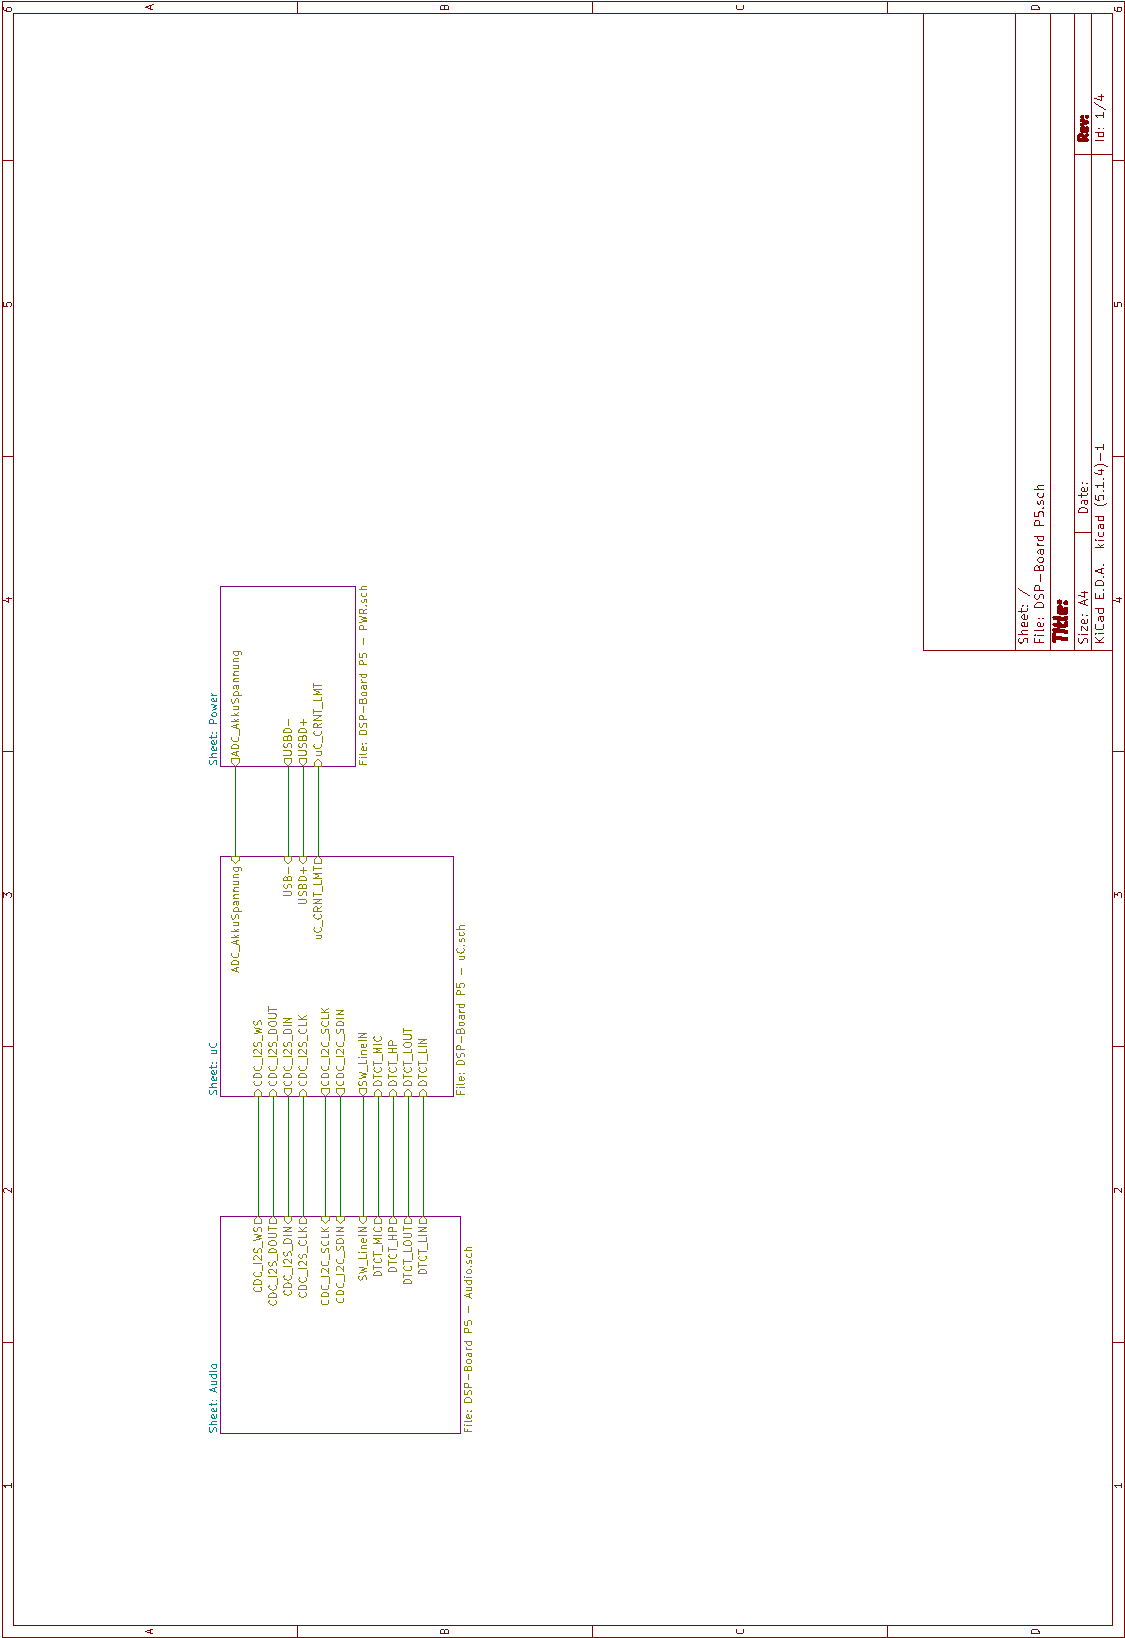
\includegraphics[width=0.95\linewidth]{appendix/DSP-Board-Schema-V1-1(1).pdf}
\end{figure}

\begin{figure}[h]
	\centering
	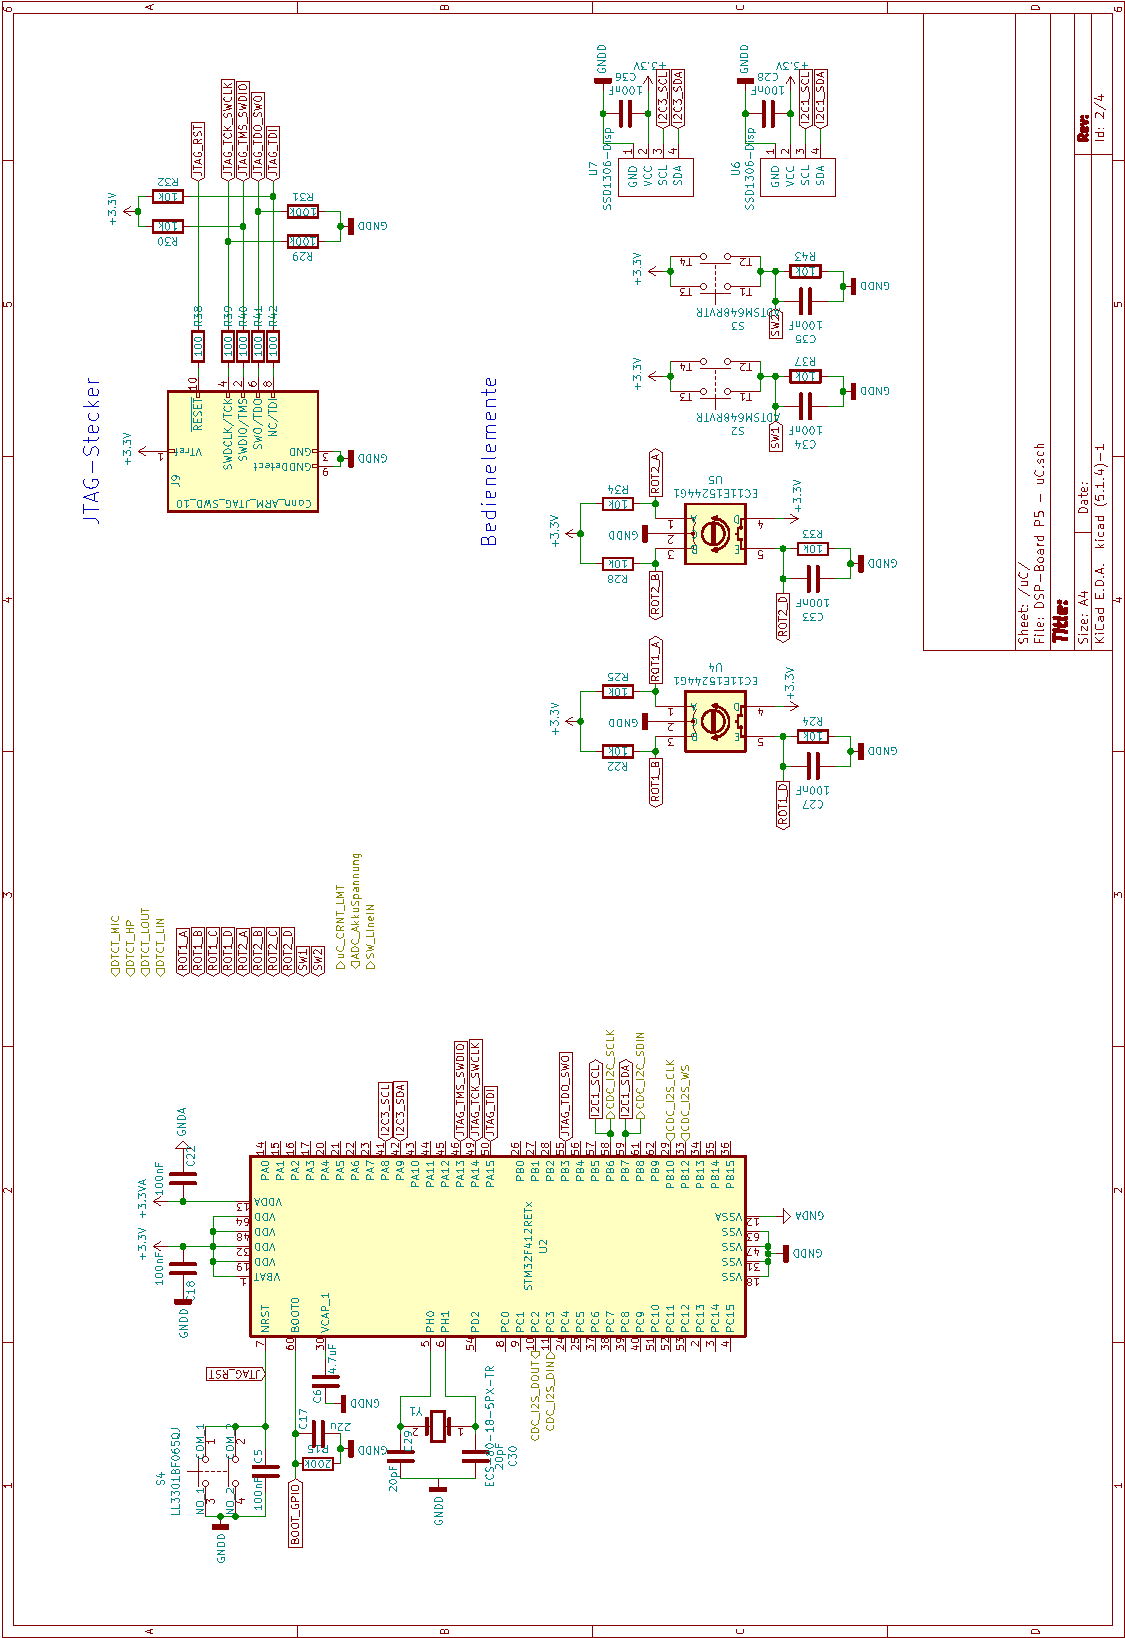
\includegraphics[width=0.95\linewidth]{appendix/DSP-Board-Schema-V1-1(2).pdf}
\end{figure}

\begin{figure}[h]
	\centering
	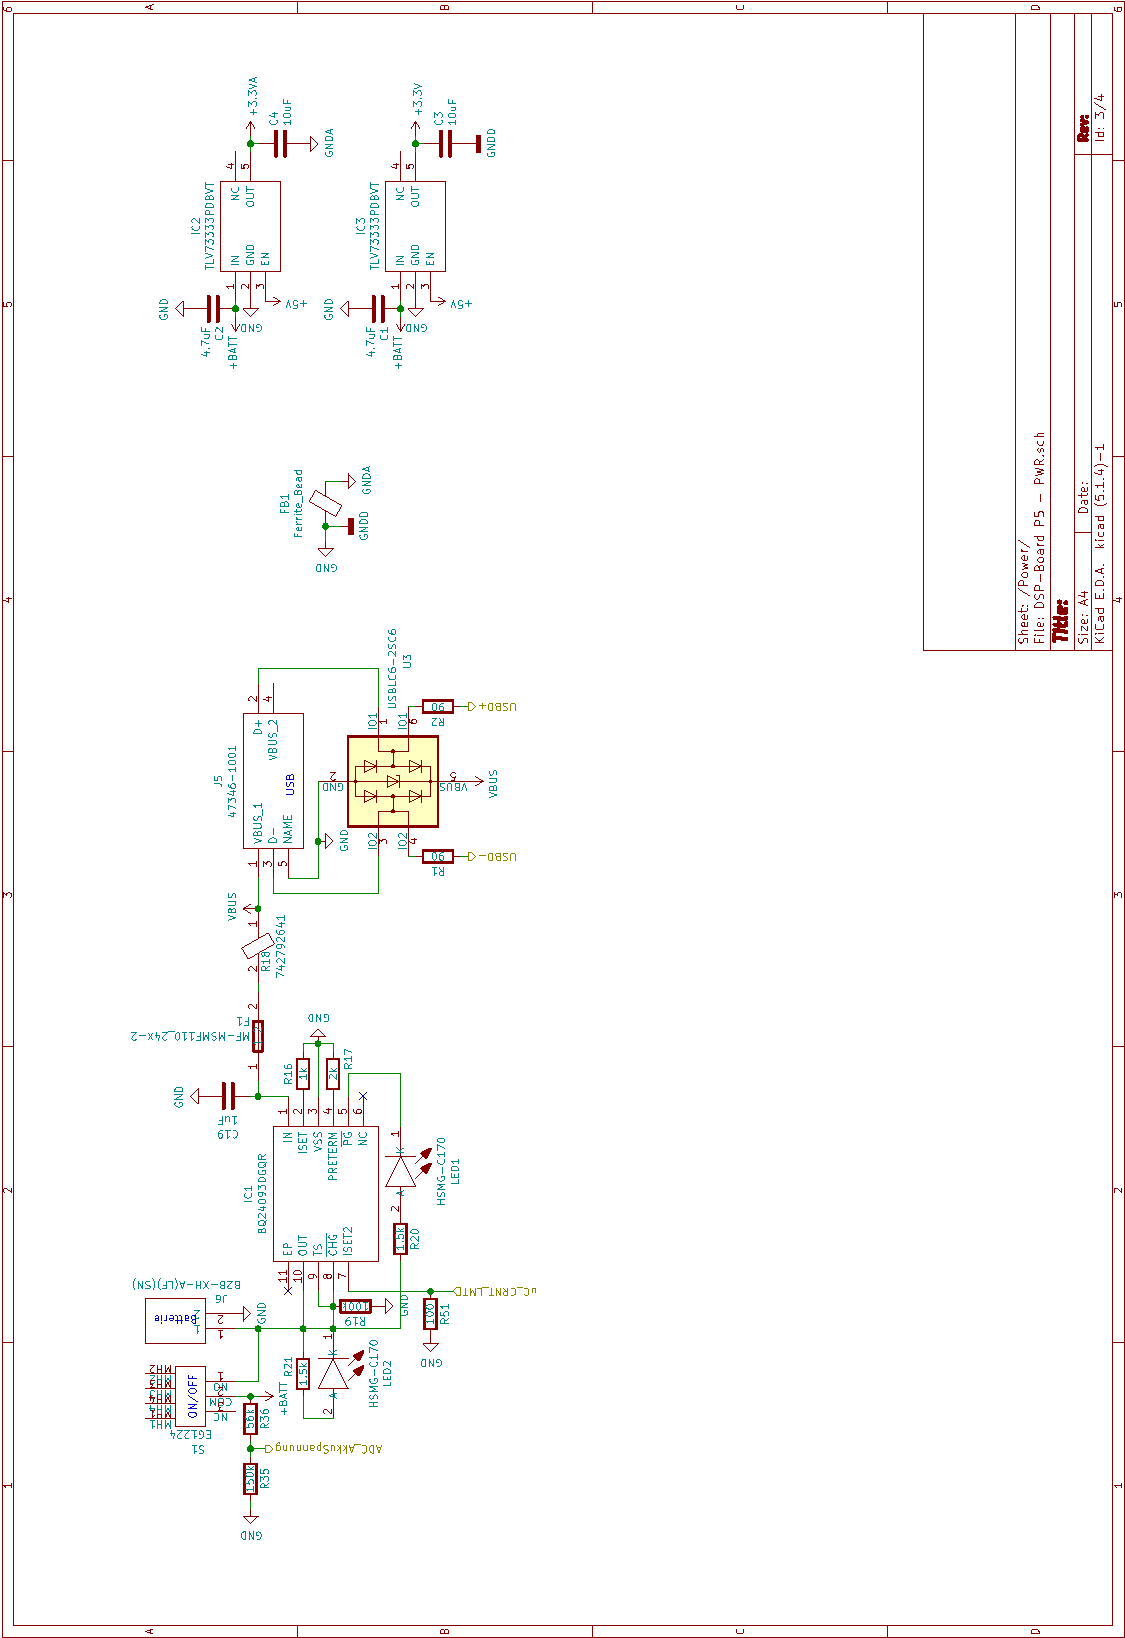
\includegraphics[width=0.95\linewidth]{appendix/DSP-Board-Schema-V1-1(3).pdf}
\end{figure}

\begin{figure}[h]
	\centering
	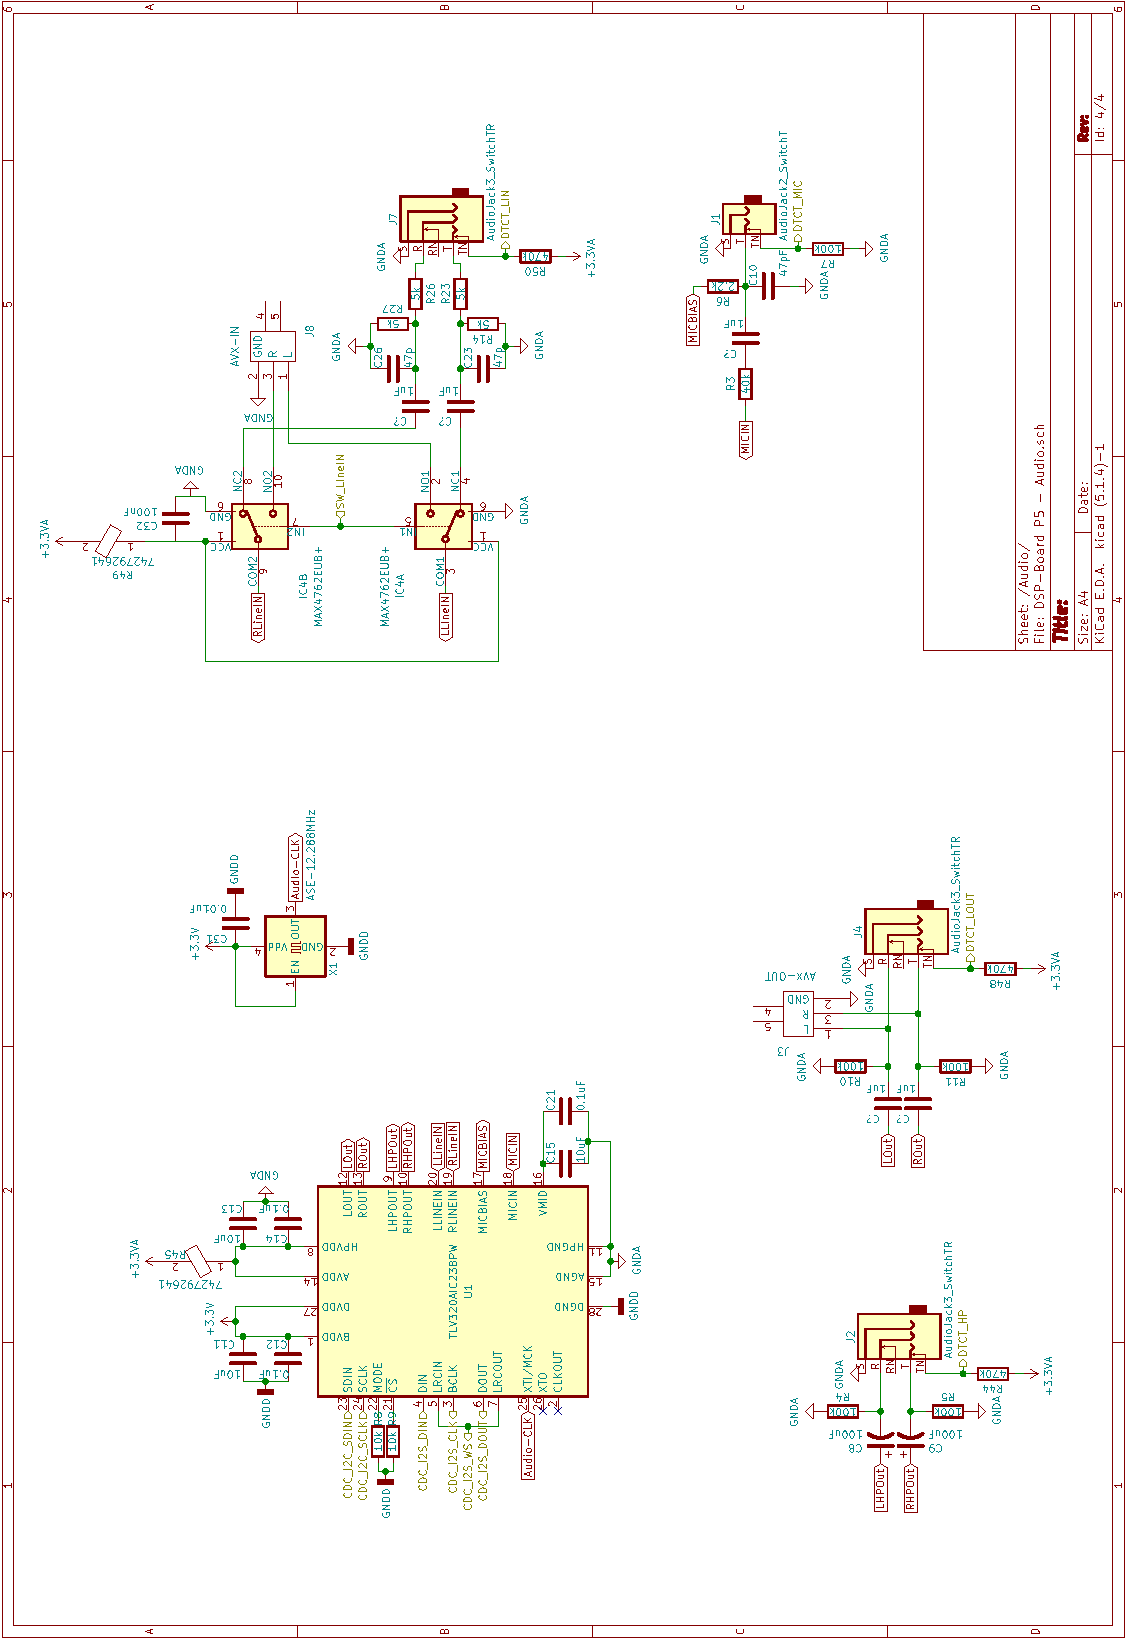
\includegraphics[width=0.95\linewidth]{appendix/DSP-Board-Schema-V1-1(4).pdf}
\end{figure}

\clearpage

\subsection{PCB Layout}
\label{app:PCB}

\begin{figure}[h!]
	\centering
	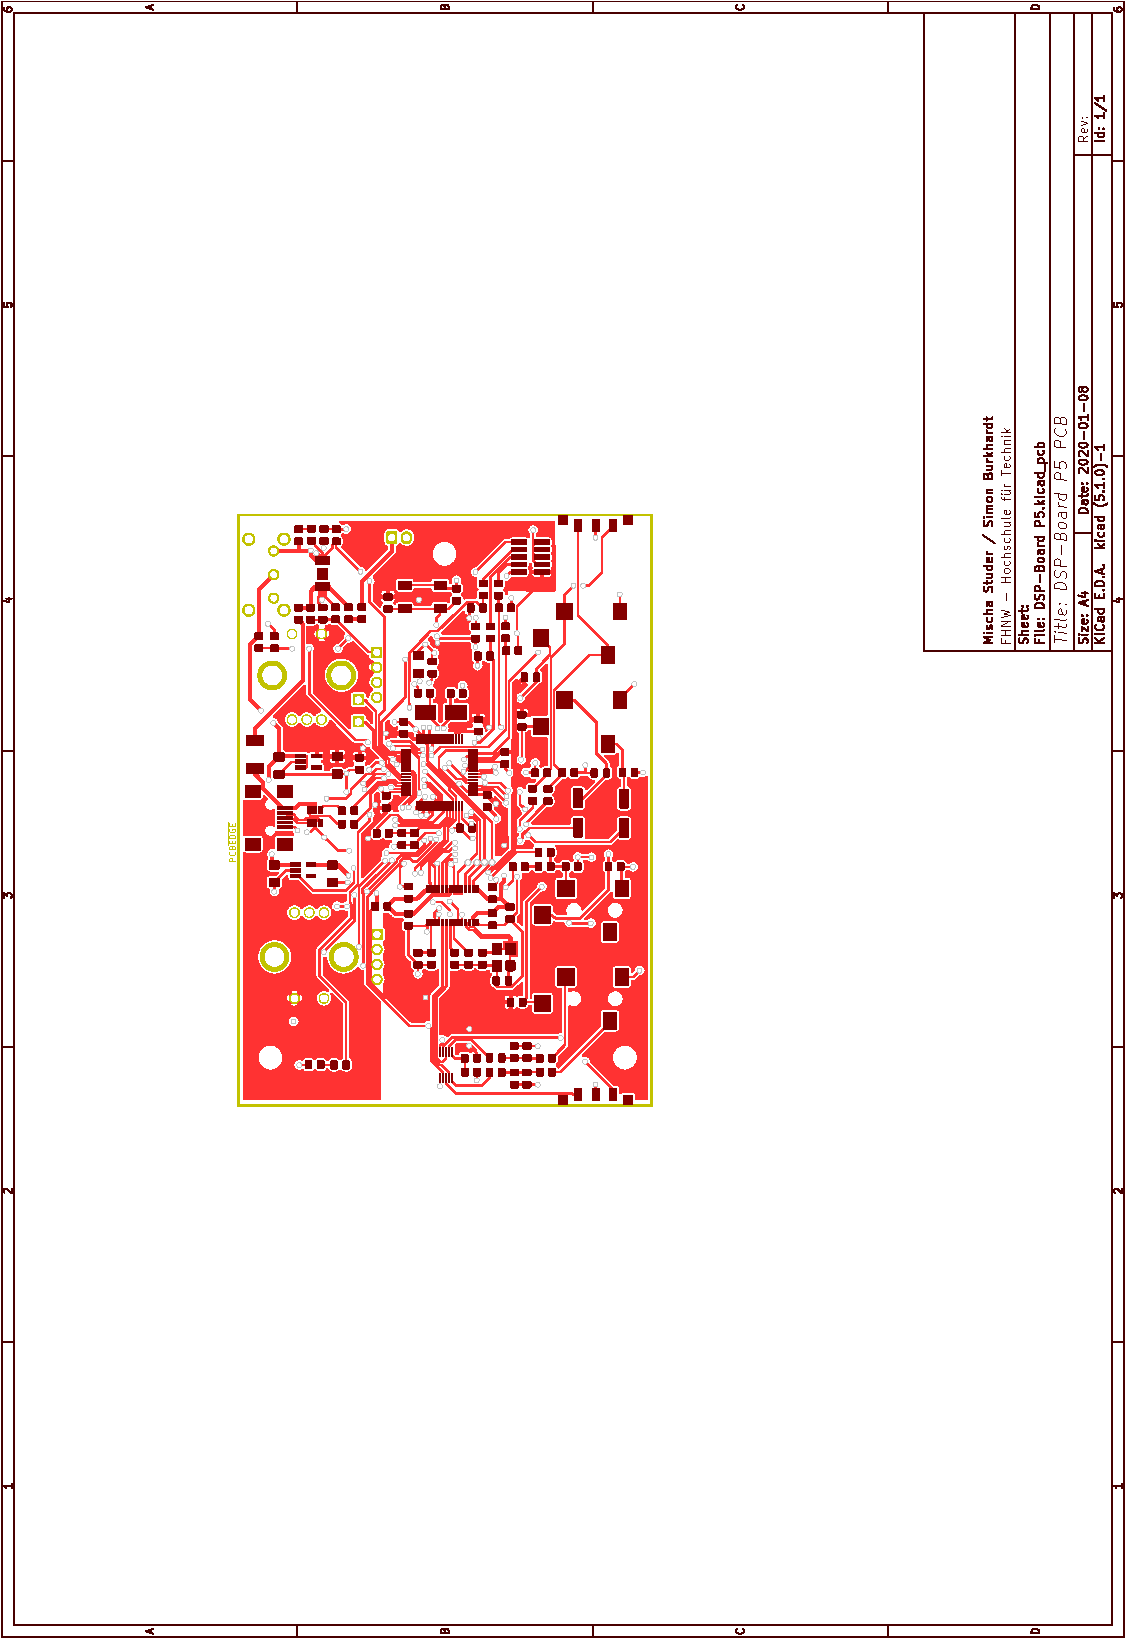
\includegraphics[width=0.95\linewidth]{appendix/DSP-Board-PCB-V1-1(1).pdf}
\end{figure}

\begin{figure}[h]
	\centering
	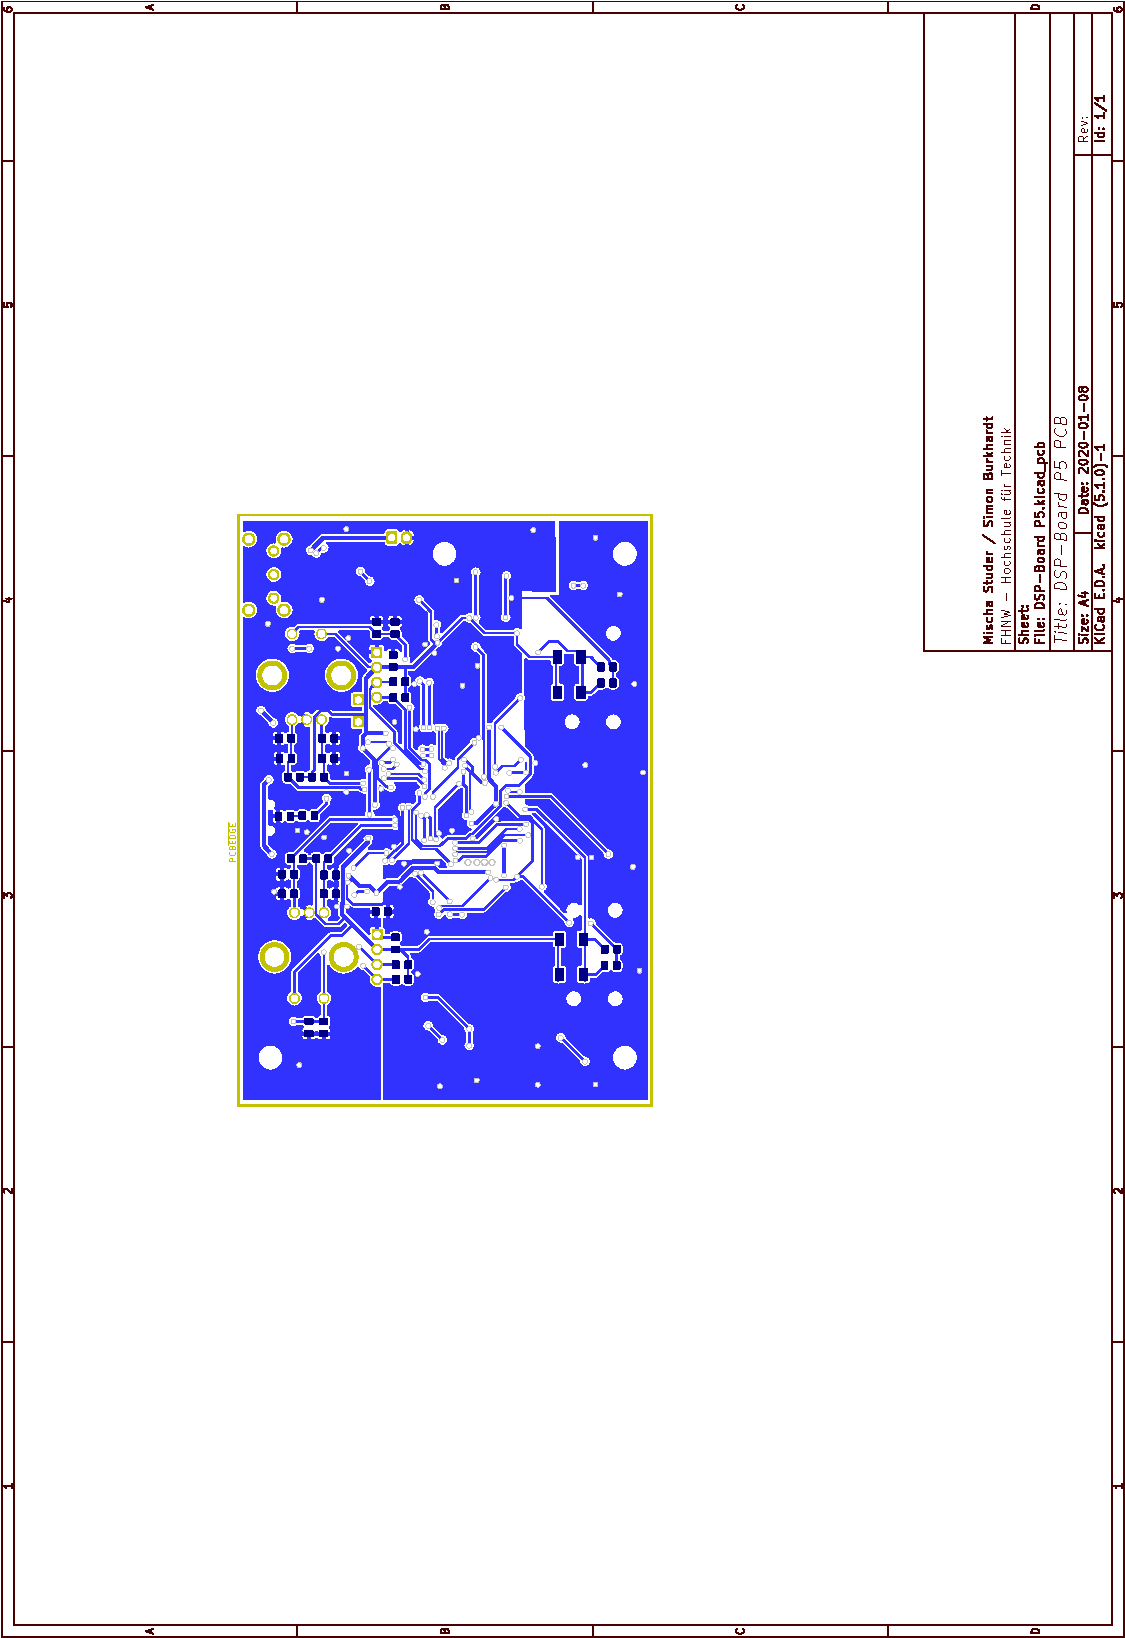
\includegraphics[width=0.95\linewidth]{appendix/DSP-Board-PCB-V1-1(2).pdf}
\end{figure}

\begin{figure}[h]
	\centering
	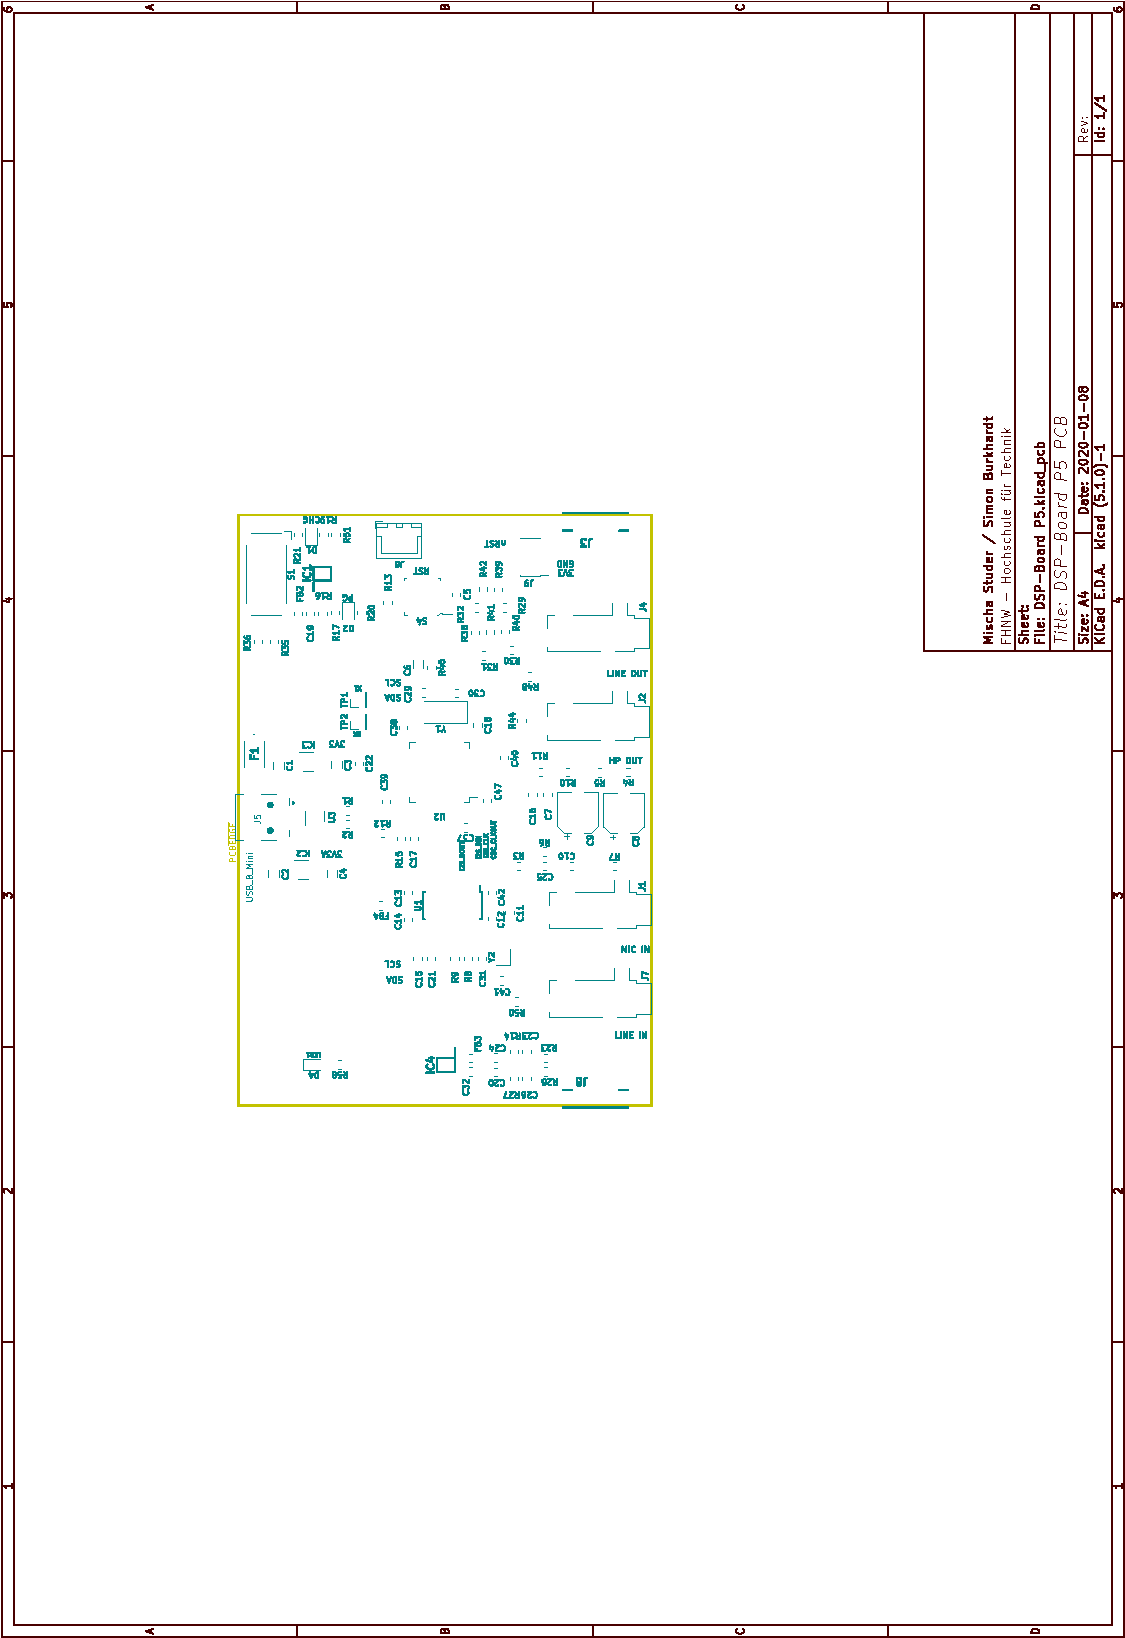
\includegraphics[width=0.95\linewidth]{appendix/DSP-Board-PCB-V1-1(3).pdf}
\end{figure}

\begin{figure}[h]
	\centering
	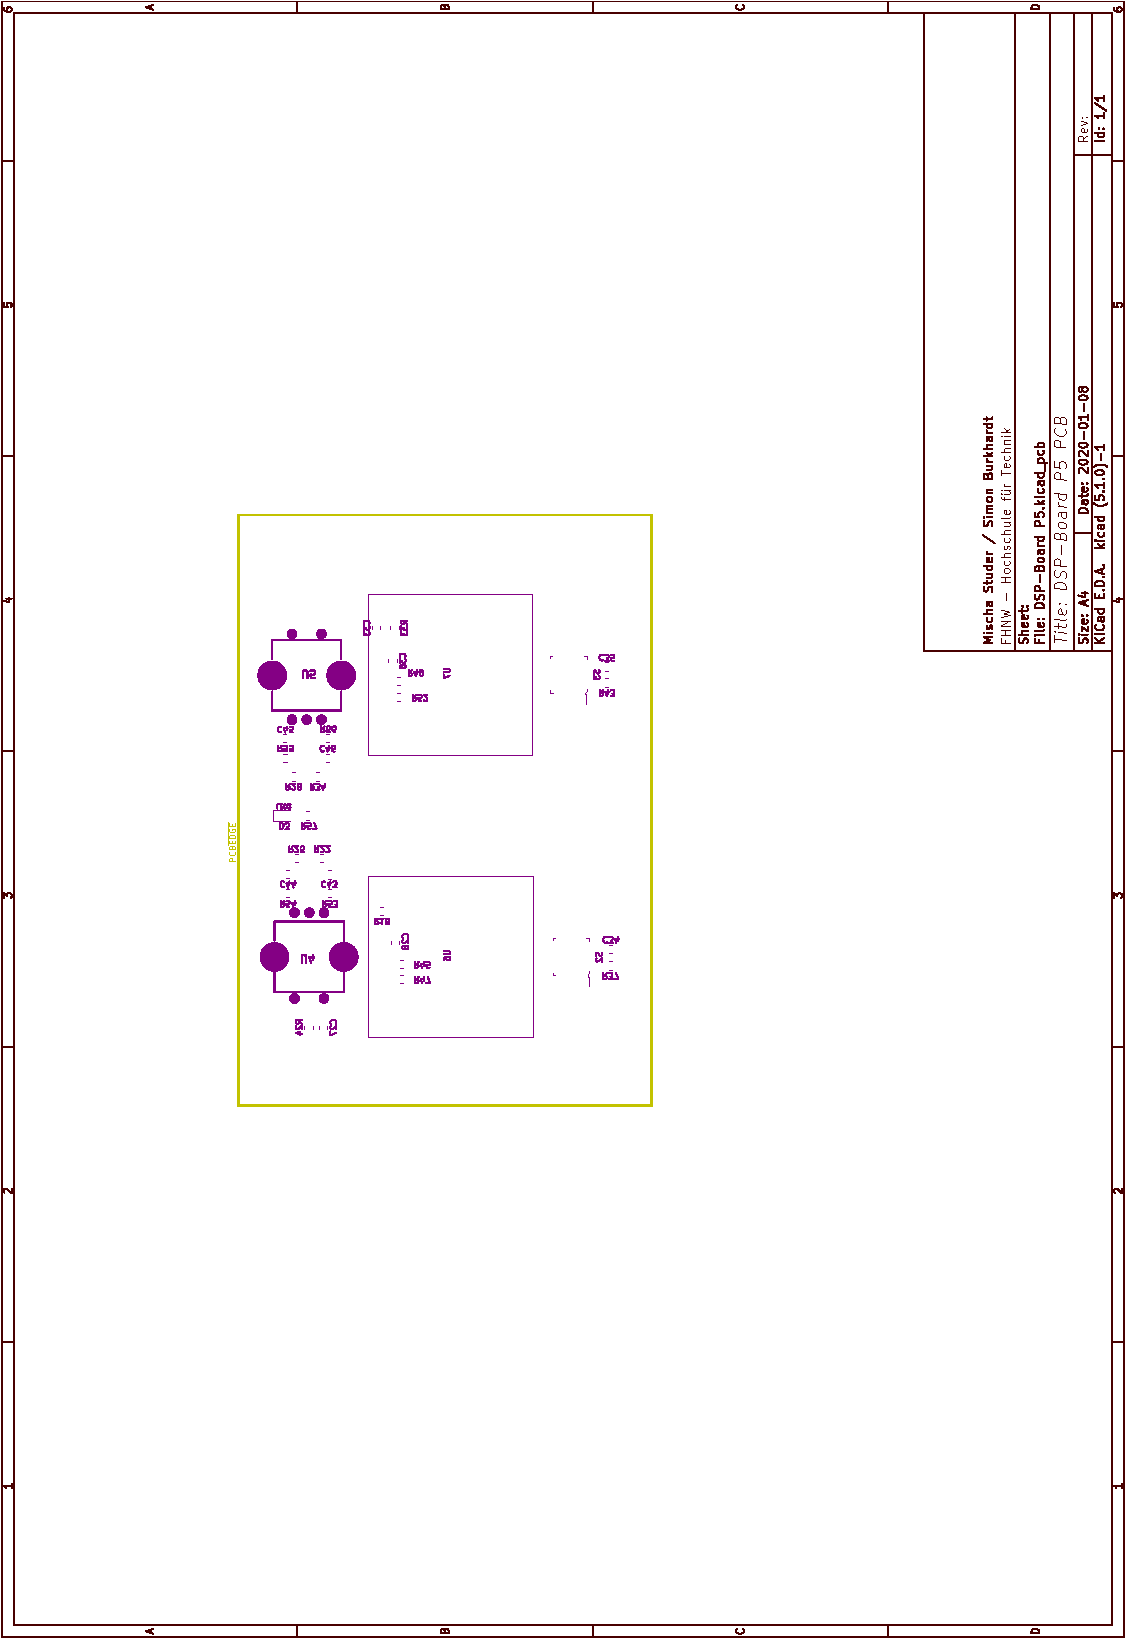
\includegraphics[width=0.95\linewidth]{appendix/DSP-Board-PCB-V1-1(4).pdf}
\end{figure}
\clearpage

\subsection{Pflichtenheft}
\label{app:Pflichtenheft}

\begin{figure}[h!]
	\centering
	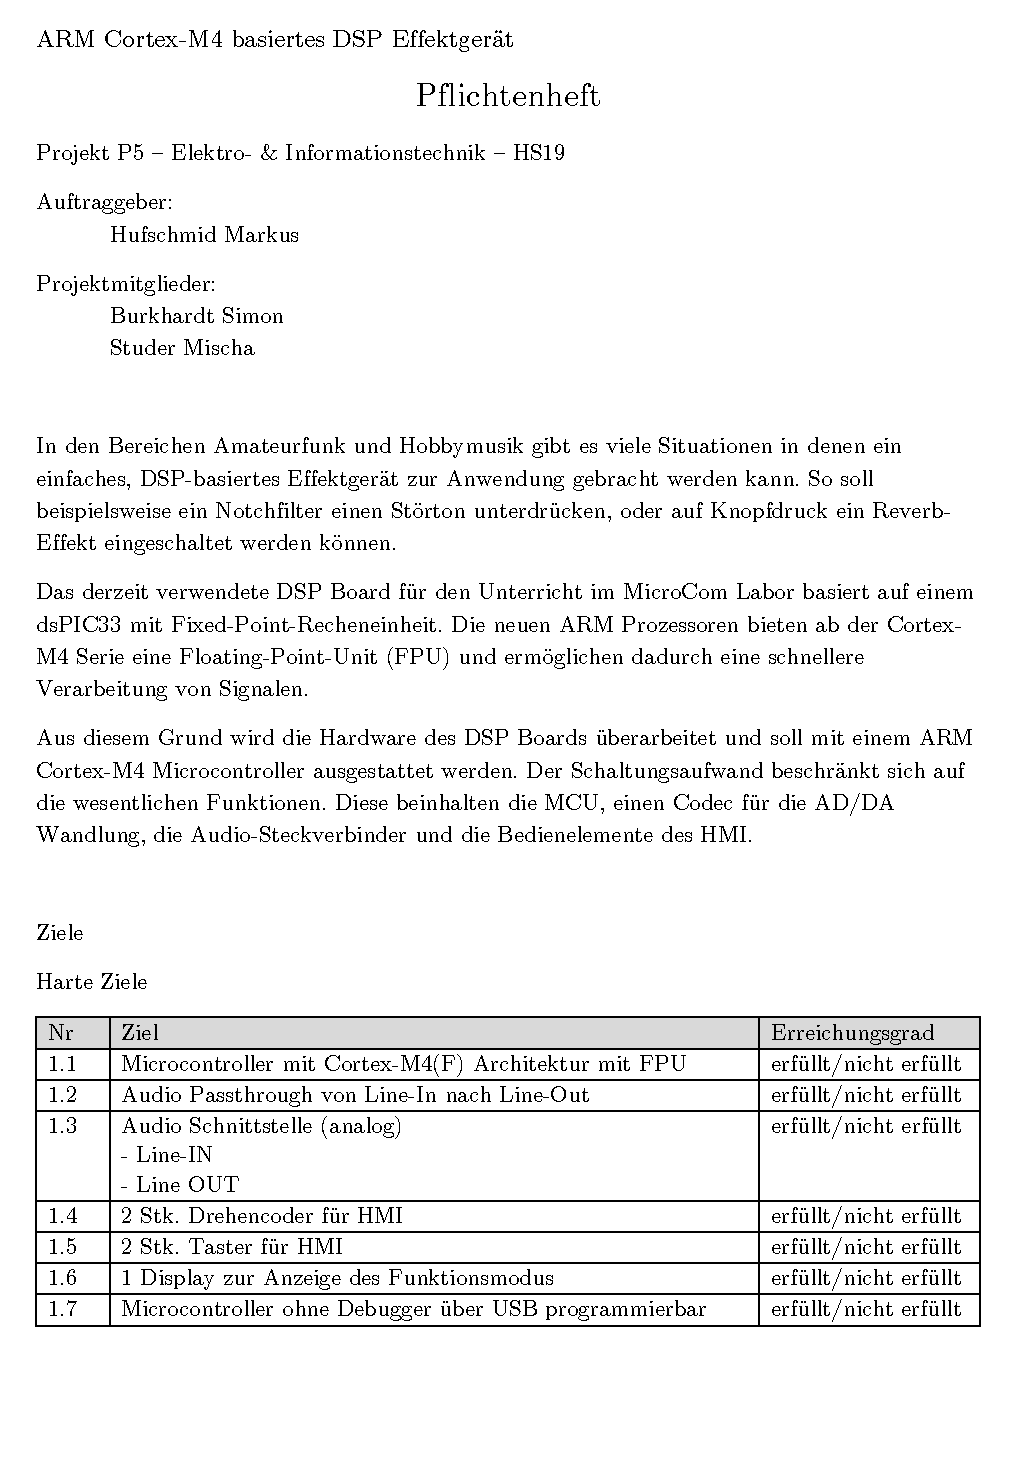
\includegraphics[width=0.95\linewidth]{appendix/pflichtenheft(1).pdf}
\end{figure}

\begin{figure}[h]
	\centering
	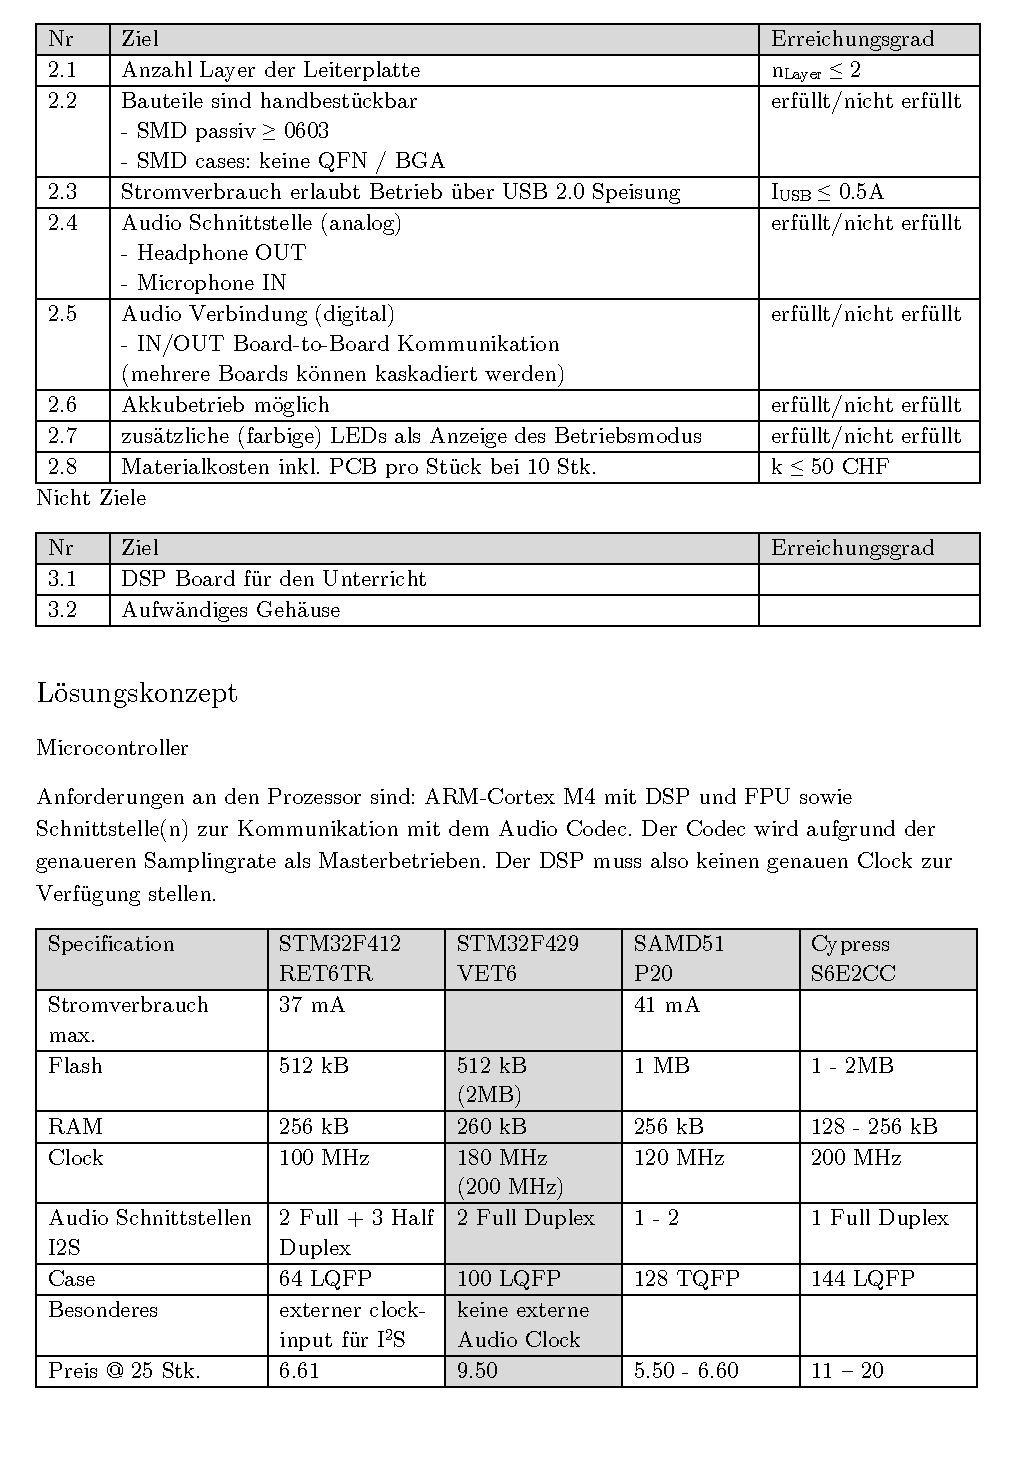
\includegraphics[width=0.95\linewidth]{appendix/pflichtenheft(2).pdf}
\end{figure}

\begin{figure}[h]
	\centering
	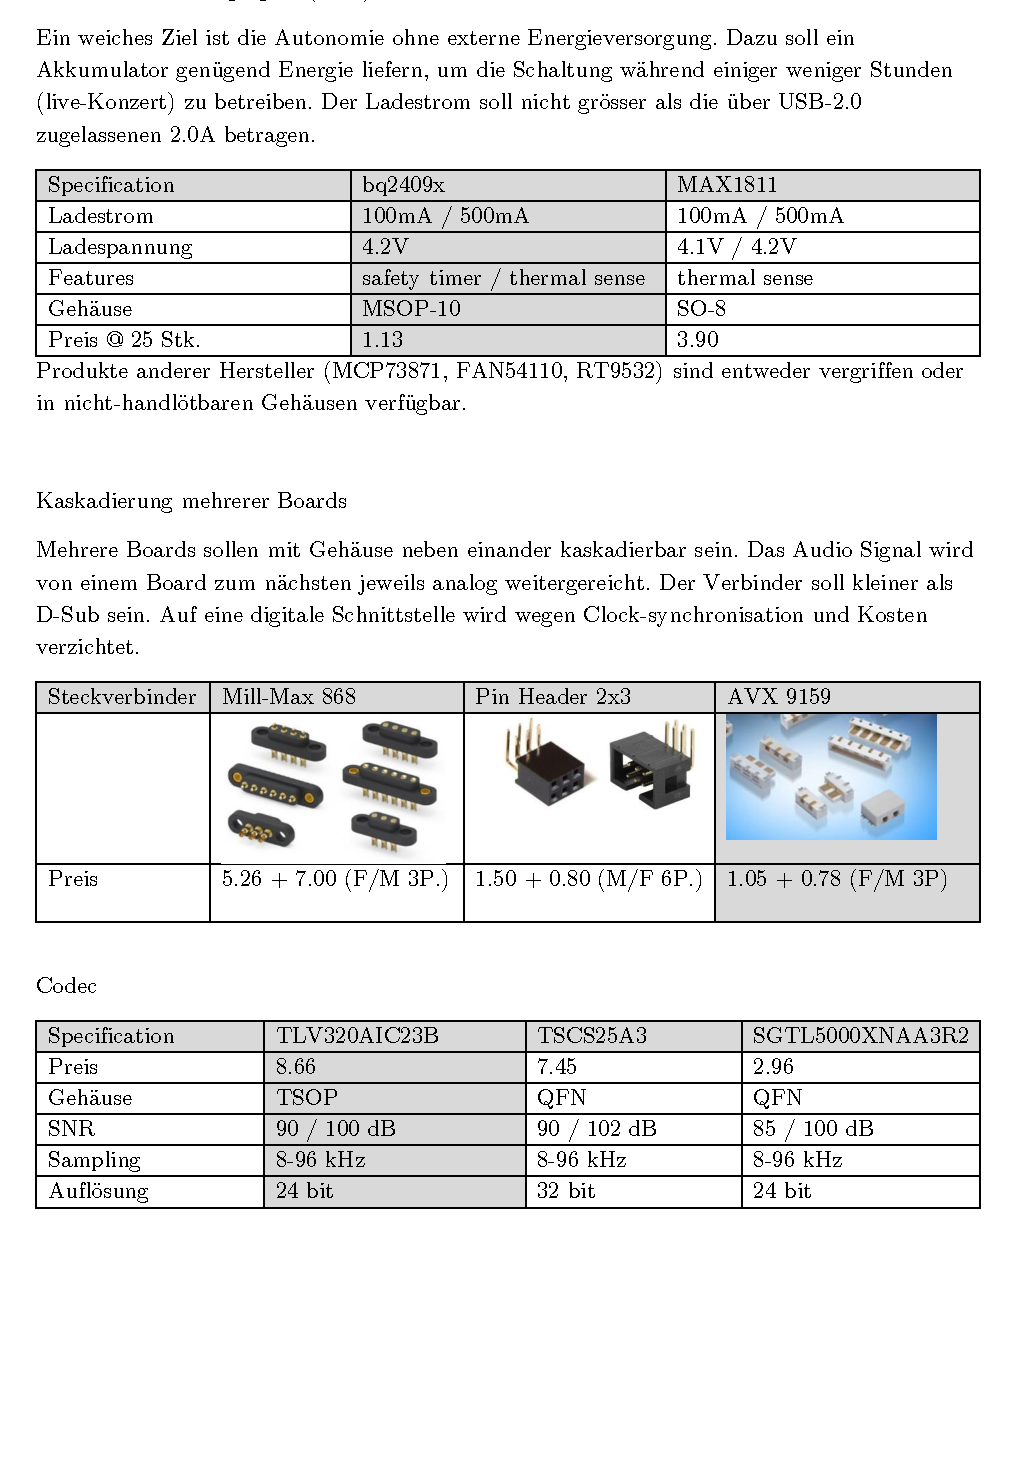
\includegraphics[width=0.95\linewidth]{appendix/pflichtenheft(3).pdf}
\end{figure}

\begin{figure}[h]
	\centering
	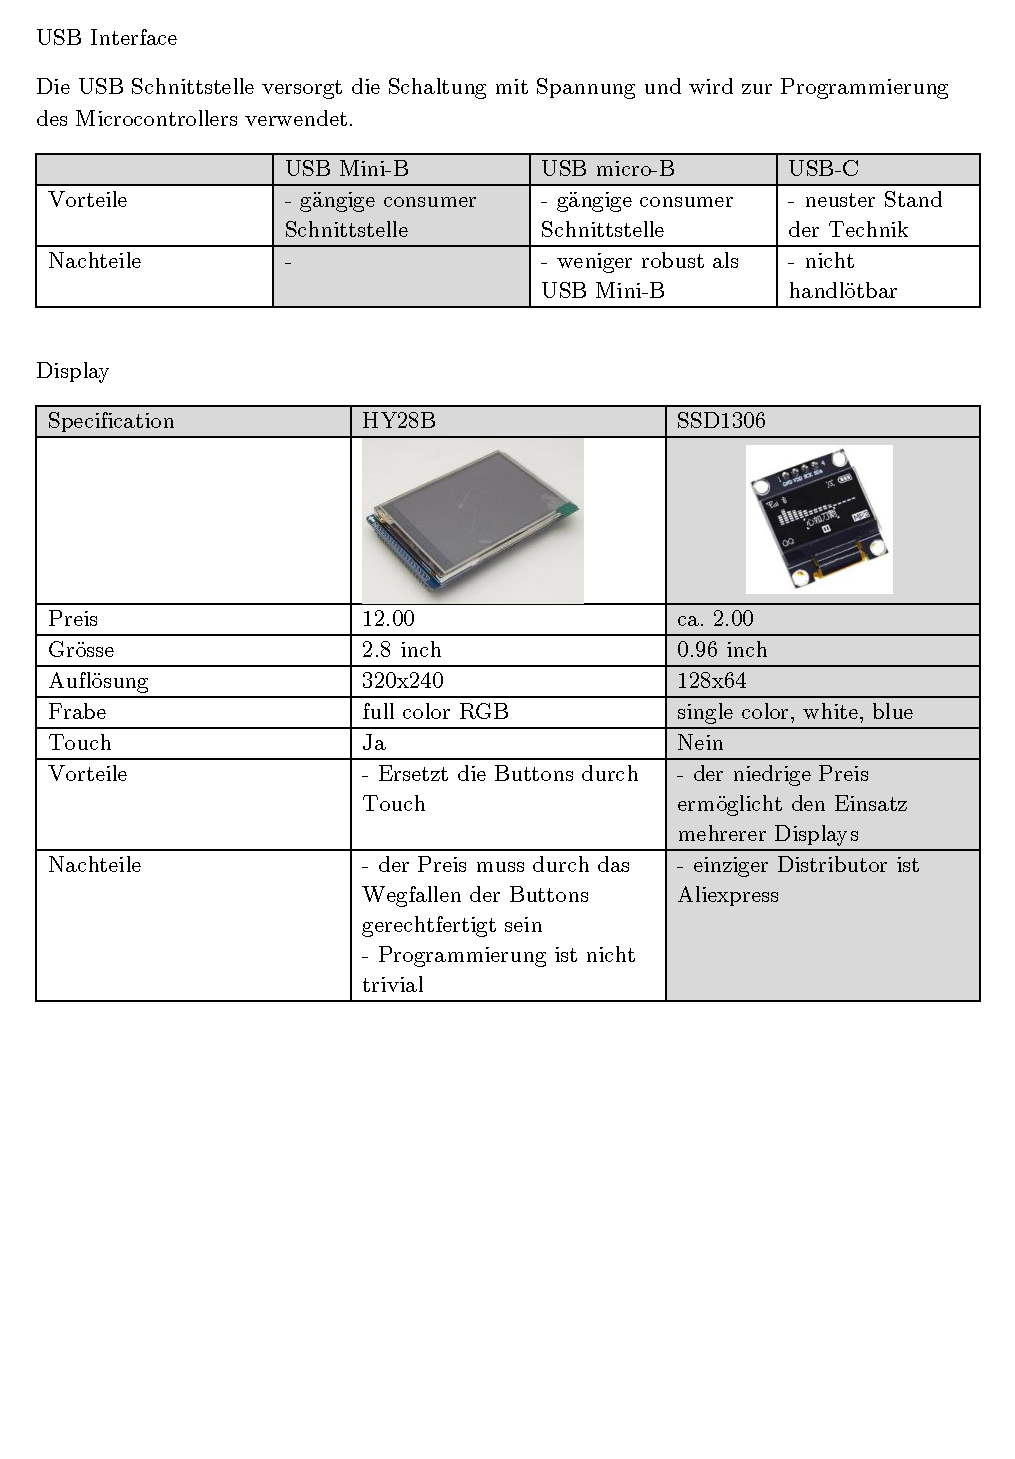
\includegraphics[width=0.95\linewidth]{appendix/pflichtenheft(4).pdf}
\end{figure}

\begin{figure}[h]
	\centering
	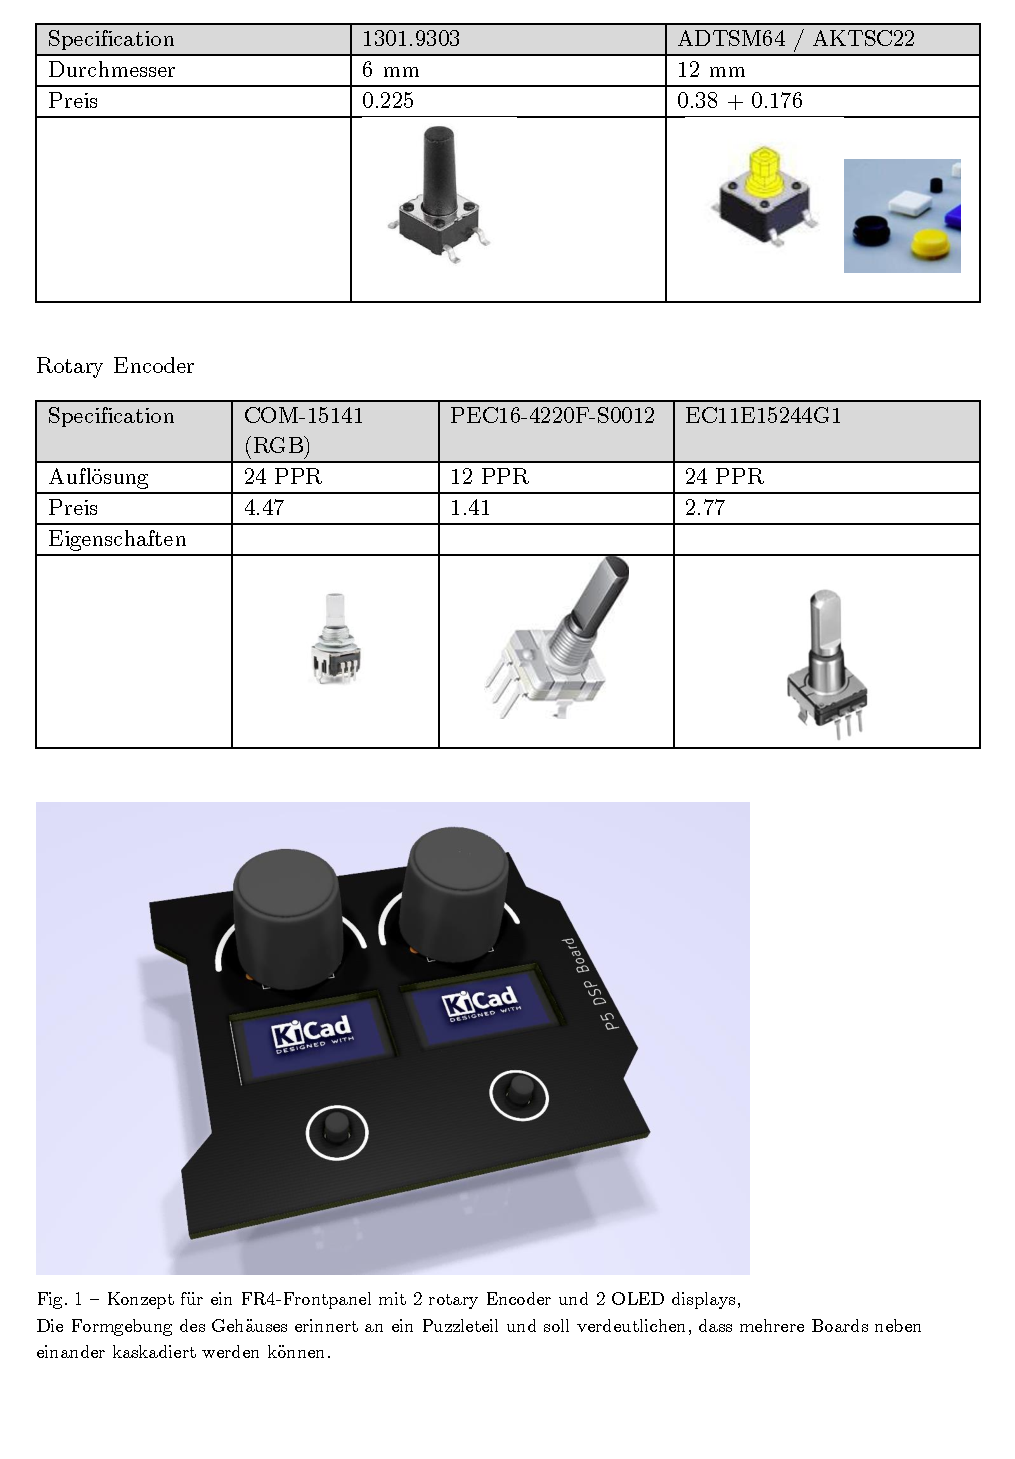
\includegraphics[width=0.95\linewidth]{appendix/pflichtenheft(5).pdf}
\end{figure}

\begin{figure}[h]
	\centering
	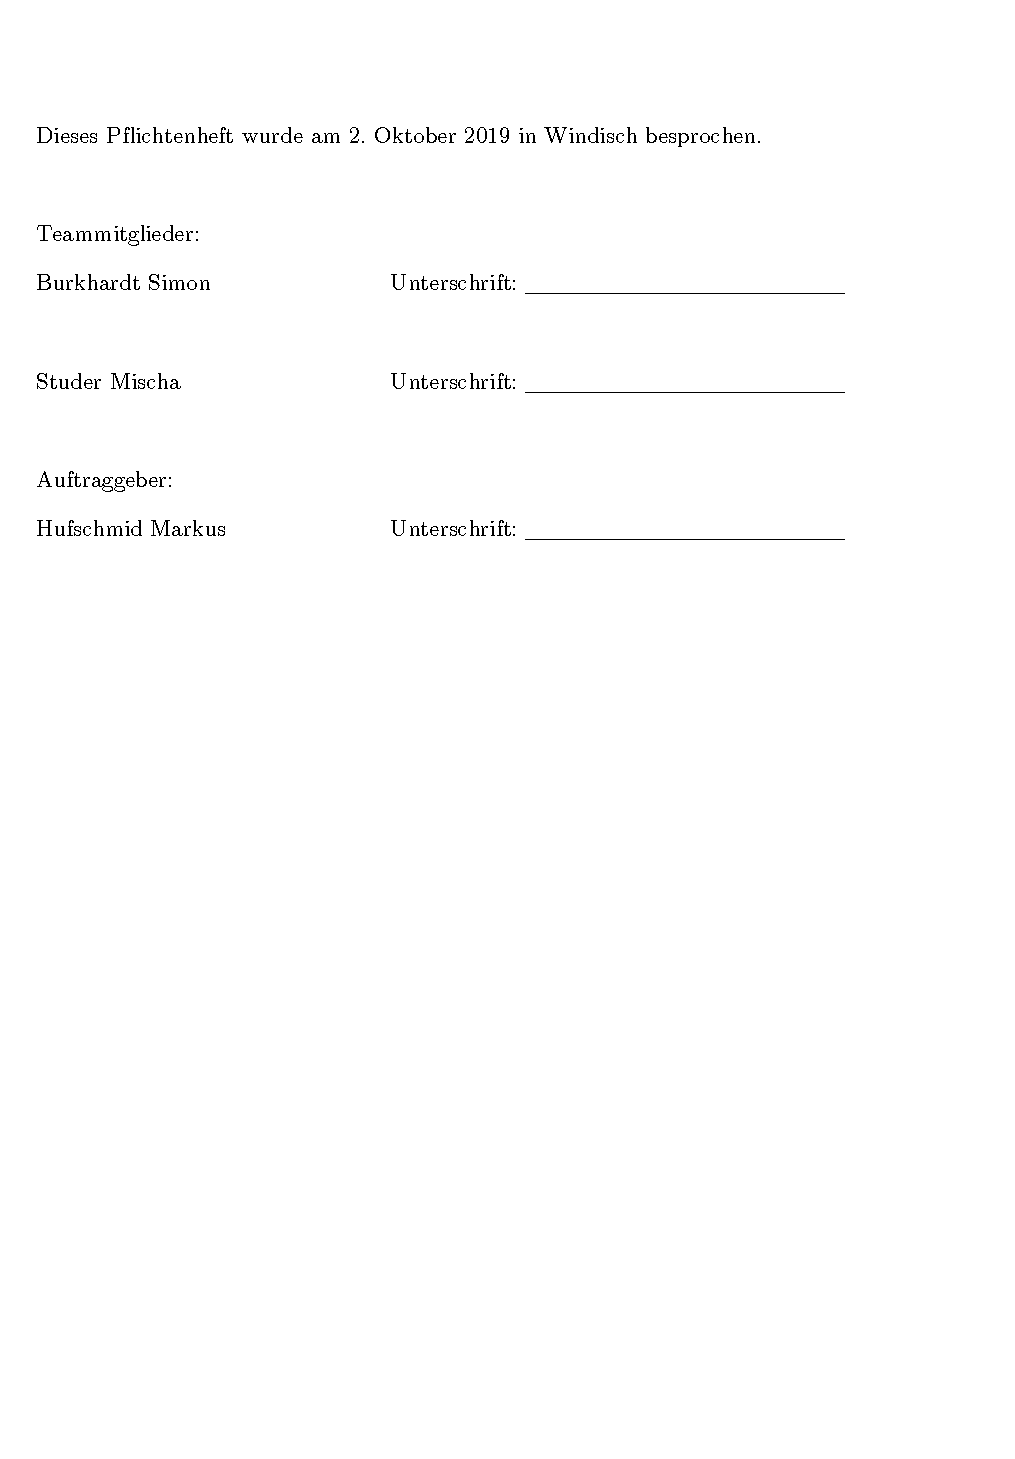
\includegraphics[width=0.95\linewidth]{appendix/pflichtenheft(6).pdf}
\end{figure}


\end{appendix}










%%---NOTES for DEBUG---------------------------------------------------------------------
%
\newpage
\listoftodos[\section{Todo-Notes}]
\clearpage


\end{document}